\subsection{Towards robust boosted jet tagging}
\label{sec:searchII:intro}
When we first studied W-tagging at 13 \TeV in context with the analysis of the 2015 dataset, Section~\ref{sec:searchI:wtagging}, two interesting correlations were observed:

\bigskip
1) A strong dependence of the AK8 CHS softdrop ($\beta = 0$) jet mass on jet \PT and

2) a strong dependence of the AK8 CHS $\tau_{21}$ cut efficiency on pileup.
\bigskip

The reason we studied the softdrop algorithm as an alternative to pruning in 2015 was, besides the possibility it would result in a higher signal efficiency, that we knew it had certain favorable qualities compared to other groomers: Softdrop removes all sensitivity to the soft divergences of QCD, by removing all soft emission, more specifically the non-global logarithmic terms (NGLs) in the jet mass~\cite{Dasgupta:2013ihk}. These arise from constellations where, for instance, a soft gluon is radiated into the jet cone, as illustrated in Figure~\ref{fig:searchII:ngls}. 

\begin{figure}[h!]
\centering
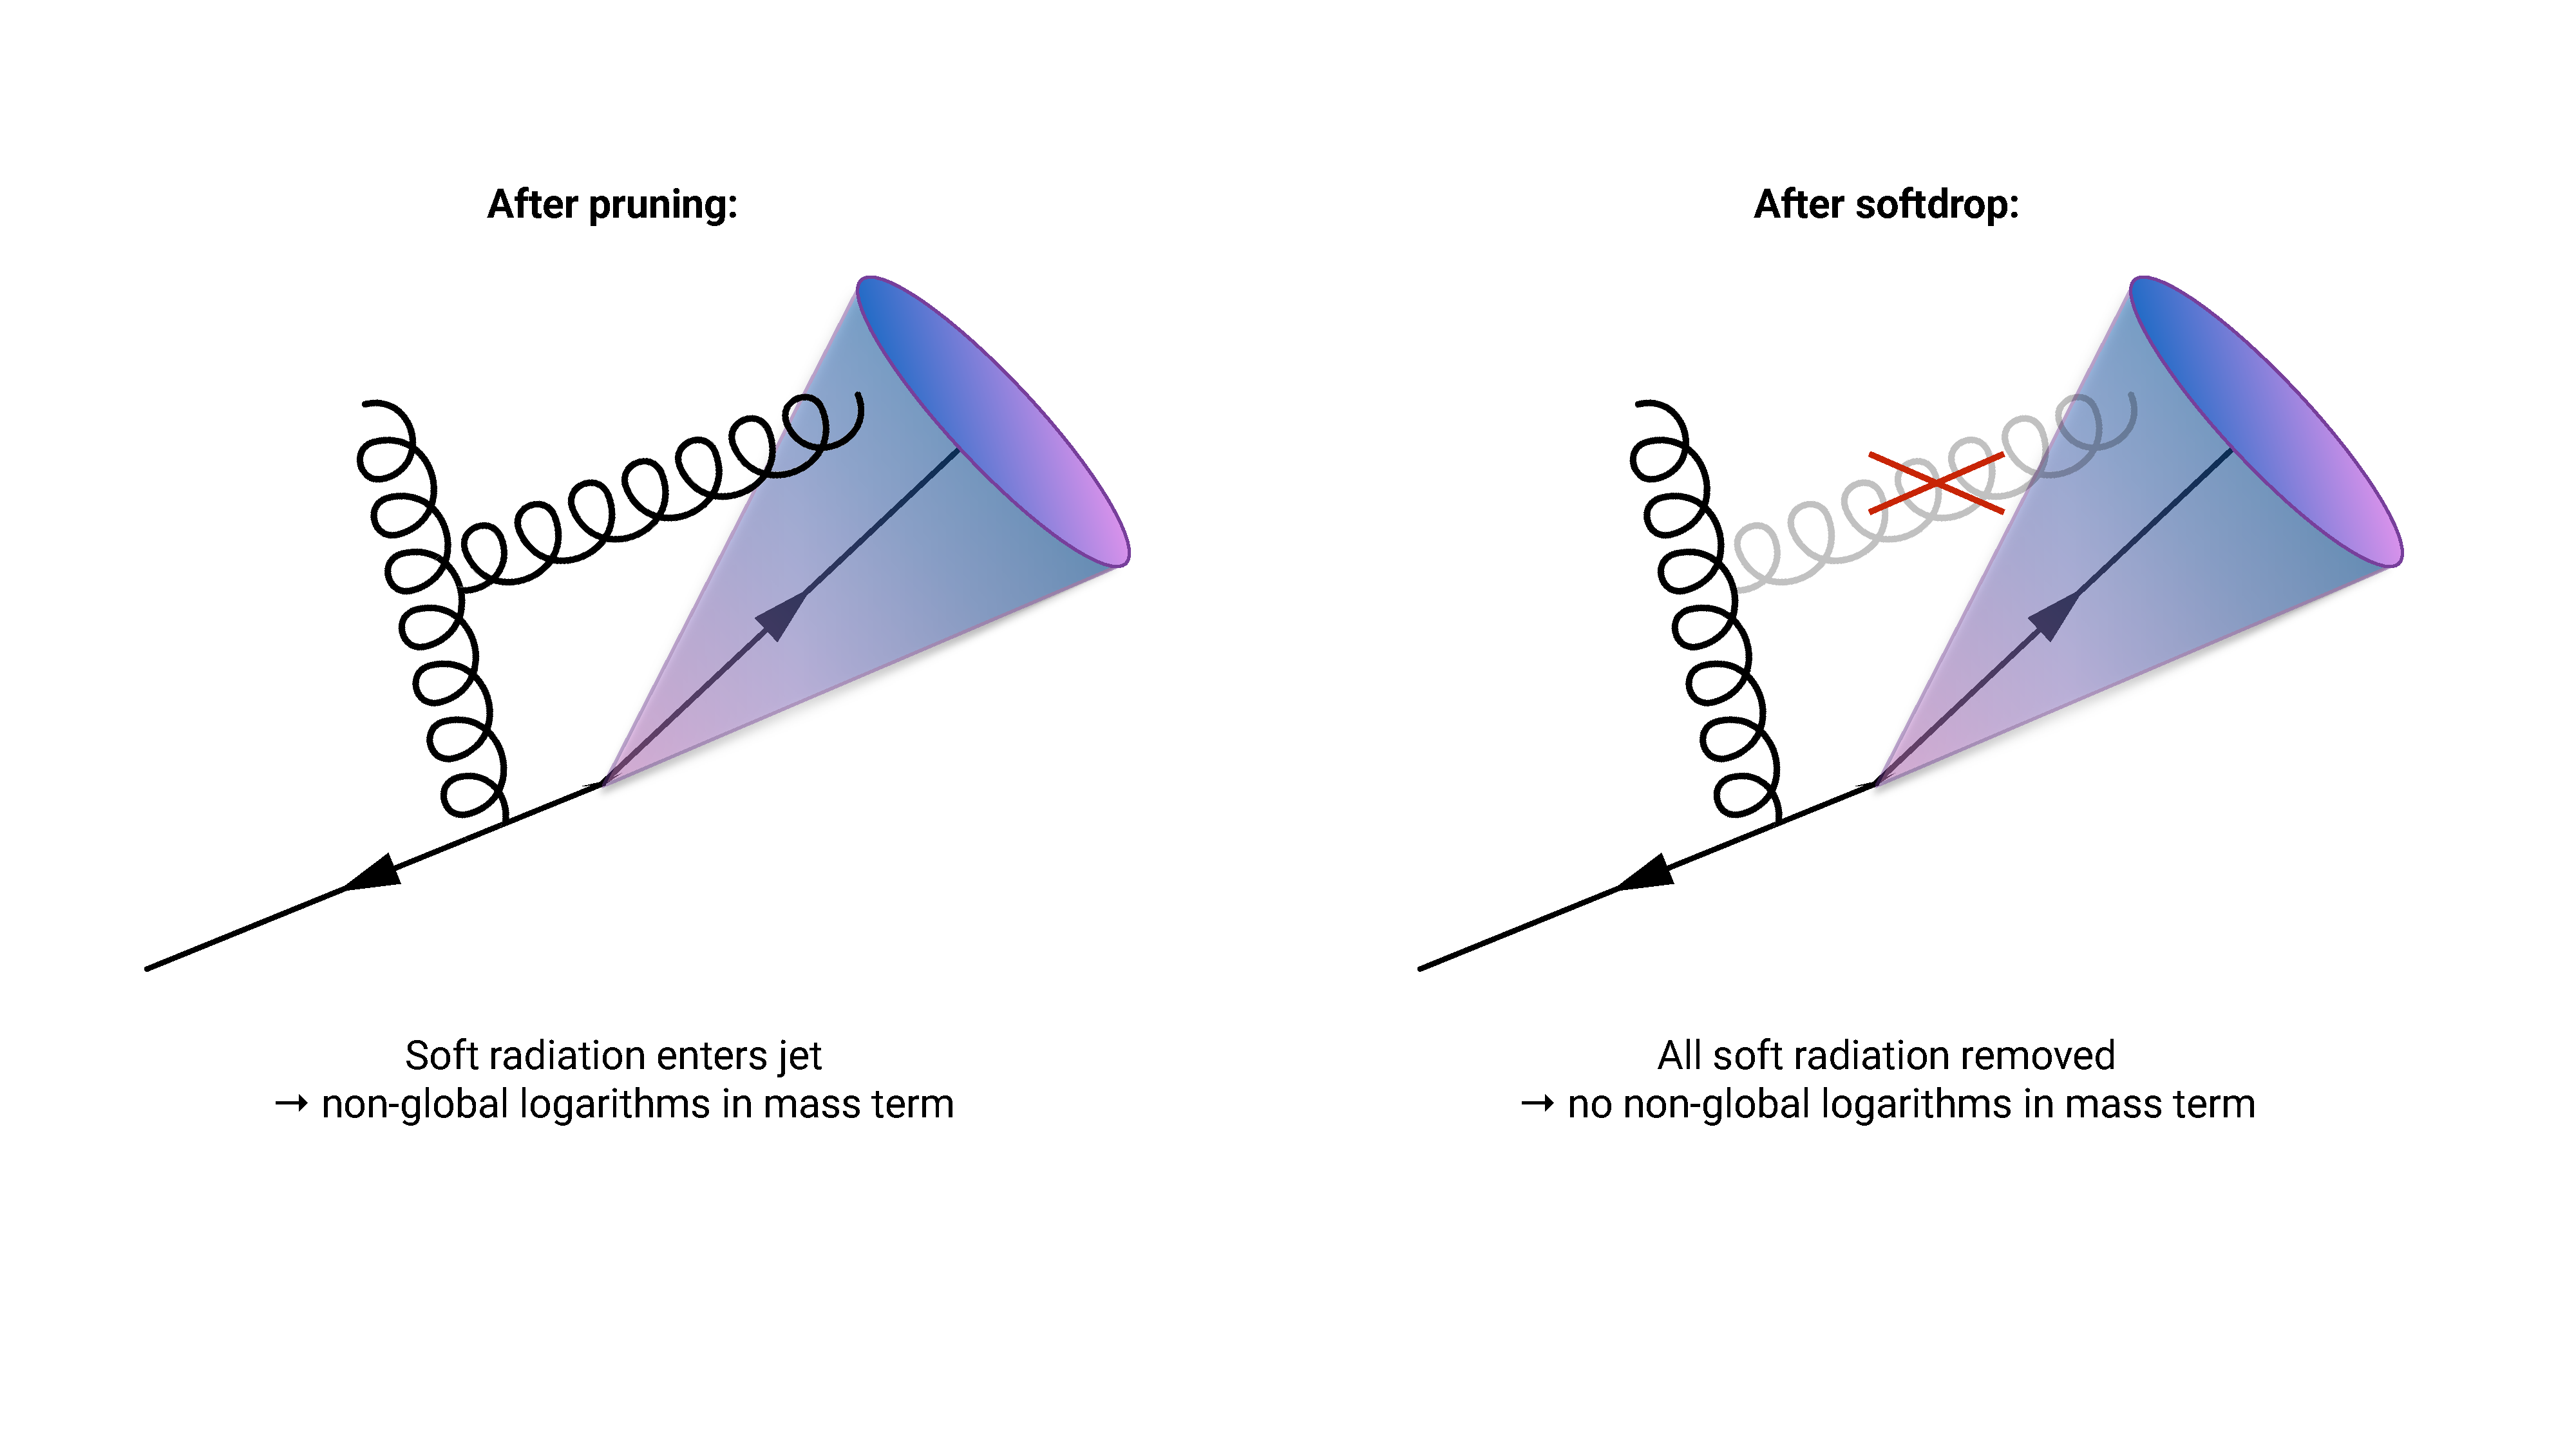
\includegraphics[width=0.69\textwidth]{figures/analysis/search2/misc/ngls.pdf}
\caption{The pruning algorithm does not remove all soft emission and therefore has non-global logarithmic terms in the jet mass. Softdrop ($\beta = 0$) completely removes soft emissions and is therefore free of non-global logarithms.}
\label{fig:searchII:ngls}
\end{figure}

The consequence of this is that you can calculate the softdrop jet mass to way higher precision than what is possible for other grooming algorithms or for the plain jet mass (NGLs are the main reason a full resummation of the plain jet mass beyond NLL (considering e.g multiple-emission effects) accuracy does not exist). Despite this not being a precision measurement analysis, we had theoretically well-motivated reasons for wanting the baseline CMS V-tagger to be softdrop-based. However, despite being less sensitive to soft radiation for QCD jets, signal jets groomed with softdrop were found to be far more sensitive to the underlying event than pruned jets~\cite{Dasgupta:2015yua}. Figure~\ref{fig:searchII:ue} shows the signal efficiency for pruning (left) and softdrop (right) as a function of jet transverse momenta when including FSR only, FSR+ISR, hadronization and hadronization + underlying event.


\begin{figure}[h!]
\centering
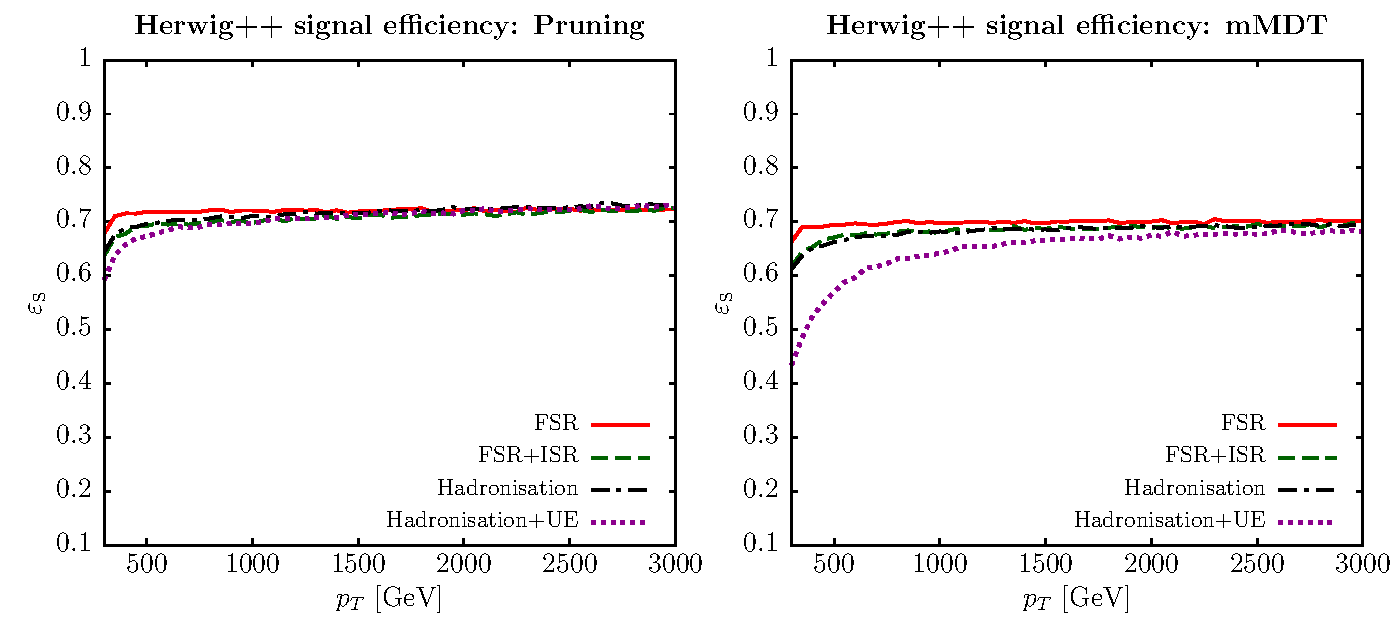
\includegraphics[width=0.79\textwidth]{figures/analysis/search2/misc/pruningvssd_ue.pdf}
\caption{The signal efficiency for pruning (left) and softdrop (right) as a function of jet \PT when adding FSR, ISR, hadronization and UE. THe UE has a severe impact on the softdrop efficiency for signal jets~\cite{Dasgupta:2015yua}. }
\label{fig:searchII:ue}
\end{figure}

On parton level, as well as after hadronization, the two algorithms perform very similar as a function of \PT. However, once UE contamination is added, the softdrop tagging efficiency is severely affected. This can be explained by the larger effective radius considered by the softdrop algorithm ( $\propto \mV/\PT \sqrt{z_{cut}(1-z_{cut})}$ ) in comparison to pruning ( $\propto \mV/\PT$ ). This observation corresponds very well with the shift in jet mass we observed for softdrop as a function of \PT in Section~\ref{sec:searchI:wtagging}: As the jet \PT decreases the softdrop effective radius increases and the jet mass mean shifts to higher values, due to absorbing more background radiation. If softdrop would be our new default tagger, a better rejection of pileup and UE contamination would be needed. In parallel to the ongoing theoretical work on groomers, a novel pileup removal algorithm had been proposed: Pileup per particle identification (PUPPI)~\cite{Bertolini2014}. Described in detail in Section~\ref{subsub:objreco:puppi}, PUPPI considers not only charged pileup but rather reweights each particle in the jet with its probability of arising from pileup. PUPPI had proven it self far superior to the current CHS algorithm in terms of jet observables for large radius jets, and therefore seemed like the obvious choice to address both issues listed above: The sensitivity of softdrop regarding UE contamination and the strong pileup dependence of $\tau_{21}$. The focus of Search II would therefore be on the commissioning of a novel W-tagger. There are interesting changes and inclusions in the analysis strategy as well: The inclusion of a $\PZpr \rightarrow \WW$ signal hypothesis and the addition of a completely new analysis, the single V-tag analysis.

\subsection{Analysis strategy}
The analysis strategy for this search is conceptually the same as for Search I. In addition, we'll take advantage of the n-subjettiness categorization and do an additional analysis in parallel: A search for excited quark resonances $\rm{q^*}$~\cite{Bauer1987,PhysRevD.42.815} decaying to qW or qZ.
We call this the single V-tag analysis, and the analysis selection only differs in that one jet is not required to pass the V-tag selection (groomed mass and n-subjettiness). The \VV analysis is hereby referred to as the double V-tag analysis. The difference between the two analyses is illustrated in Figure~\ref{fig:searchII:svsd}. 

\begin{figure}[h!]
\centering
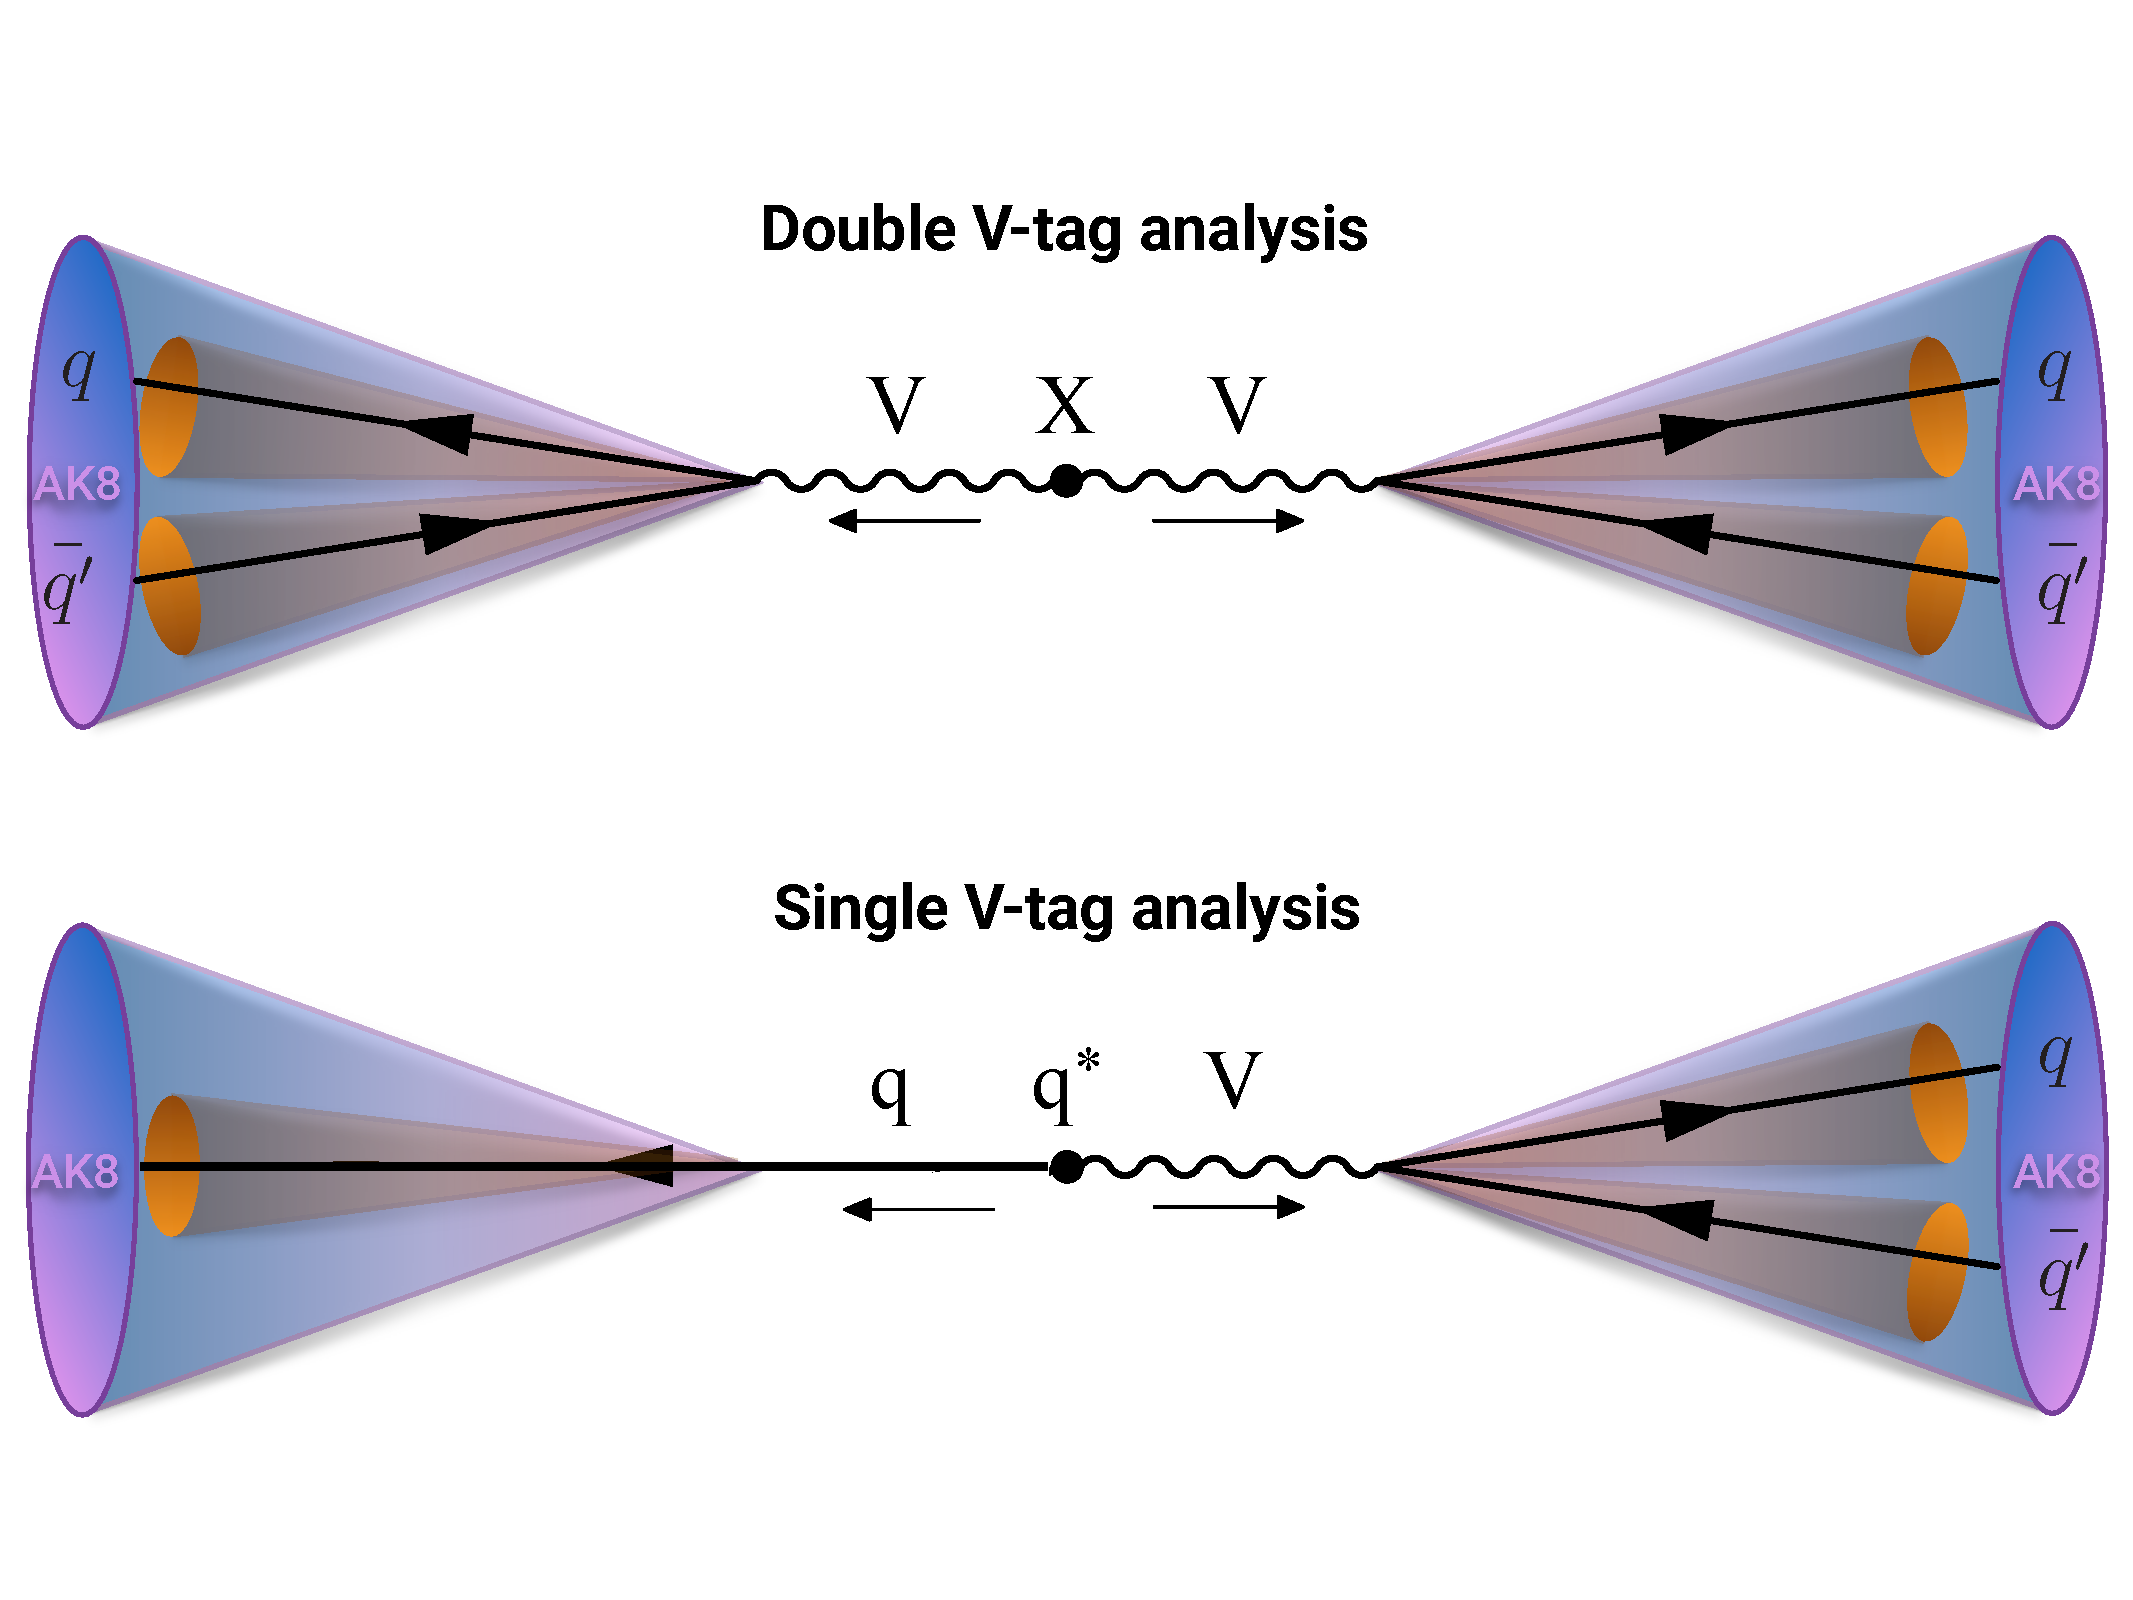
\includegraphics[height=6.5cm]{figures/analysis/search2/misc/singlevsdoubletag.pdf}
\caption{The double (top) and single (bottom) W/Z-tag analysis.}
\label{fig:searchII:svsd}
\end{figure}

In addition, limits are set on a $\PZpr \rightarrow \WW$ signal hypothesis in the double V-tag analysis, another 13 \TeV first.\newline
This analysis was published in two steps: An early Physics Analysis Summary (PAS) based on 12.9 \fbinv of 2016 data~\cite{CMS-PAS-B2G-16-021}, describing the new  PUPPI+softdrop based V-tagger as well as the single V-tag analysis, and a second analysis topping up with the full 2016 data~\cite{PhysRevD.97.072006}. The commissioning of the new \PW\PZ-tagger has also been documented in a jet performance Physics Analysis Summary~\cite{CMS-PAS-JME-16-003}. As the new V-tagger was developed and commissioned in the context of the early analysis, which was also were the single V-tag analysis was first published with 13 \TeV data, the main emphasis will be on the work presented in CMS-PAS-B2G-16-021~\cite{CMS-PAS-B2G-16-021}. The second part of the results chapter, Section~\ref{}, includes the results obtained using the full 2016 dataset of 35.9 \fbinv.

\subsection{Data and simulated samples}
\label{sec:searchII:samples}
As mentioned above, the analysis of the 2016 dataset was done in two steps: One based on 12.9 \fbinv of early 2016 data describing the new W-tagger and single V-tag category, and a second topping up with the full 2016 dataset, corresponding to 35.9 \fbinv.\par
The \BulkG and HVT signal samples are modeled in precisely the same way as in 2015. For the single V-tag $\textrm{q}^*$ samples, we simulate unpolarized boson with a compositeness scale $\Lambda$ set equal to the resonance mass. These are generated to leading order using \PYTHIA version 8.212~\cite{Sjostrand:2007gs}. \par
The background Standard Model processes; QCD, W+jets and Z+jets are all simulated to leading order. V+jets is simulated with \amcatnlo~\cite{Alwall:2014hca,Alwall:2007fs}, while three different combinations of matrix element and shower generators is used for QCD as these predictions are known to differ: \PYTHIA only, the leading order mode of \amcatnlo{} matched with \PYTHIA, and \HERWIG{++}~2.7.1~\cite{Bahr:2008pv} with tune CUETHS1~\cite{Khachatryan:2015pea}.

\subsection{Event selection}

\subsubsection{Triggering}

The triggers used in this analysis are the same ones as in 2015 (see Section~\ref{sec:searchI:trigger}), however, due to the new single V-tag analysis, the trigger turn-ons have this time been re-evaluated separately requiring either one or two jets to have an offline softdrop jet mass above 65 \GeV.
\par Figure~\ref{fig:searchII:trigger-fits} shows the trigger turn-on curves as a function of dijet invariant mass for jets passing one of the three inclusive triggers only, one of the grooming triggers only and when combining all of them. The turn-on curves are shown for all jet pairs passing loose selections as described in Section \ref{sec:searchI:preselection}. Zero, one or two of the two jets is further required to have a softdrop mass larger than 65 GeV.

\begin{figure}[h!]
\centering
% 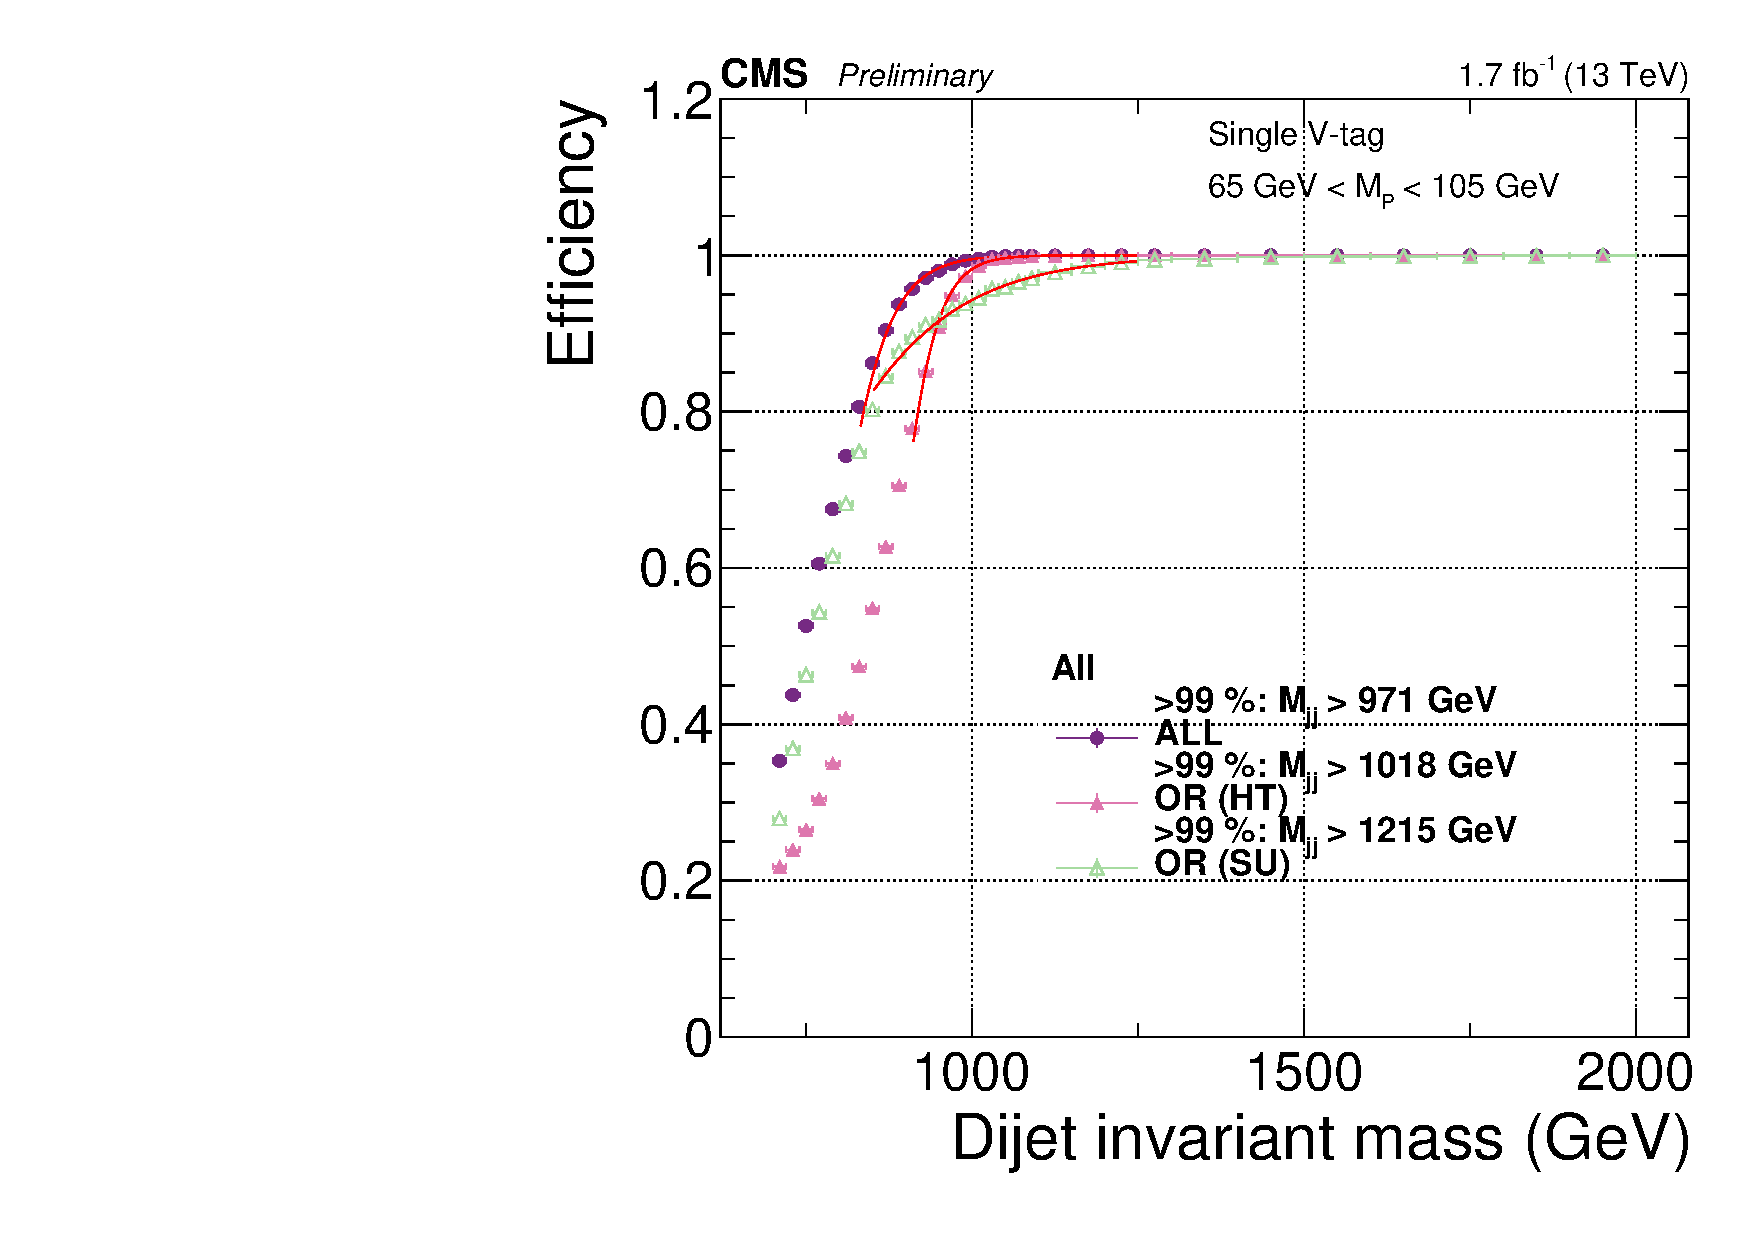
\includegraphics[width=0.4\textwidth]{figures/analysis/search2/AN-16-398/plots/trigger/triggereffMjj-ALL_SingleTag_runAll.pdf}
% 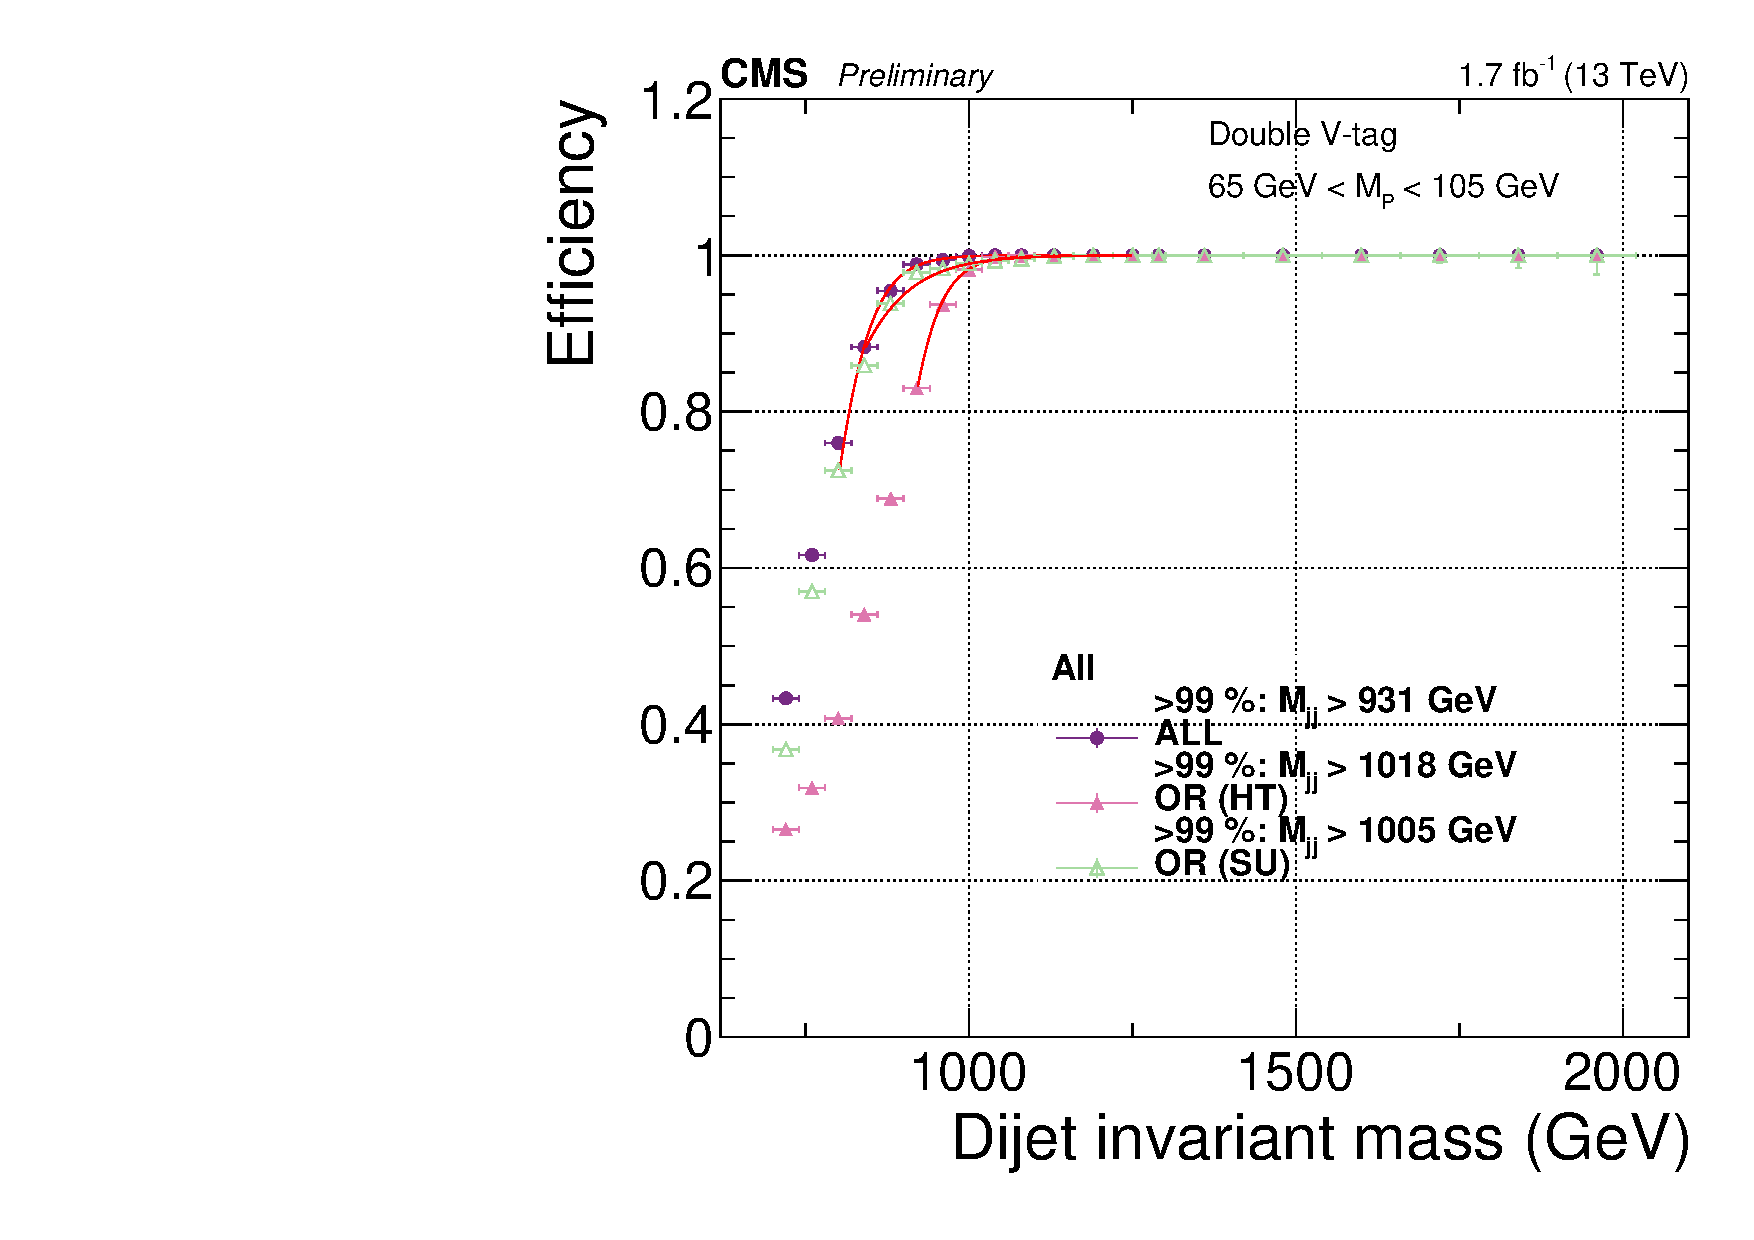
\includegraphics[width=0.4\textwidth]{figures/analysis/search2/AN-16-398/plots/trigger/triggereffMjj-ALL_DoubleTag_runAll.pdf}
% 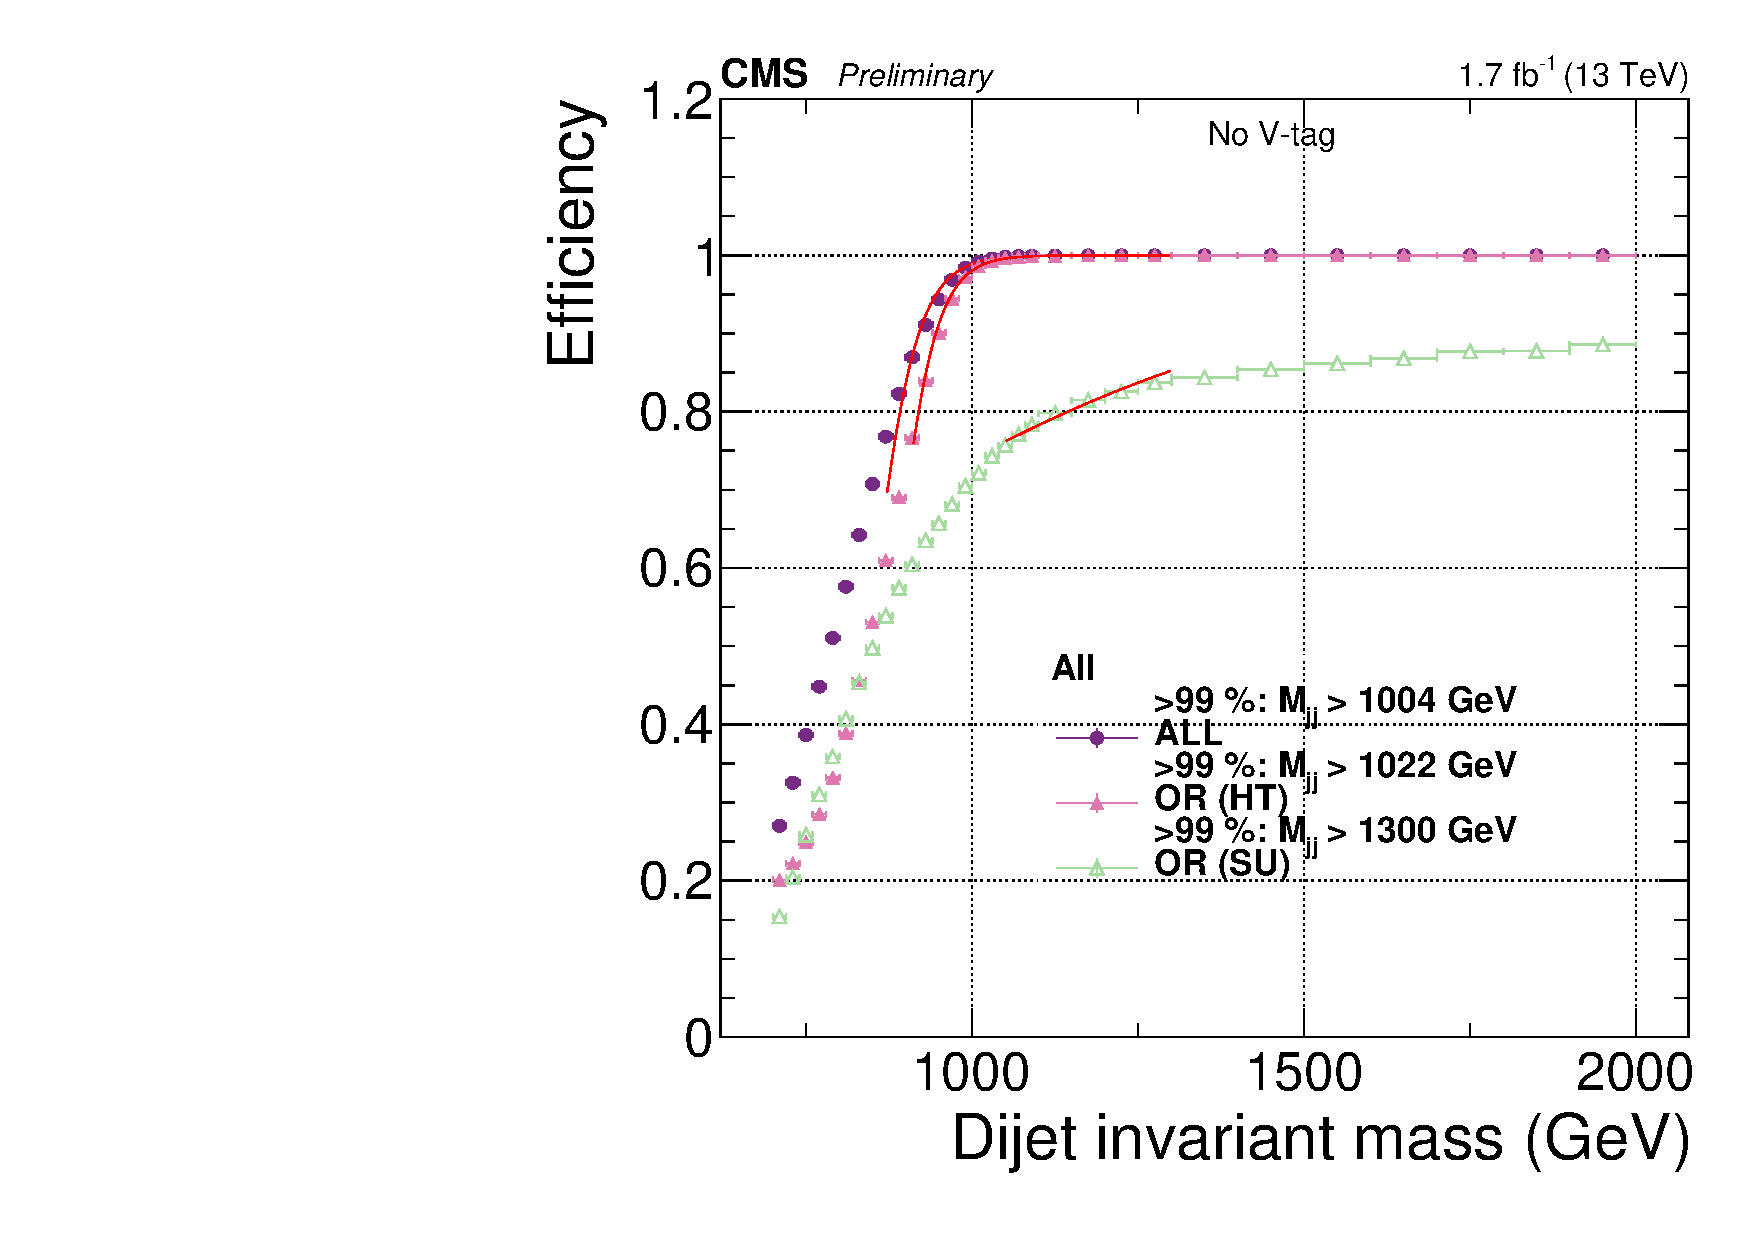
\includegraphics[width=0.4\textwidth]{figures/analysis/search2/AN-16-398/plots/trigger/triggereffMjj-ALL_noTag_runAll.pdf}
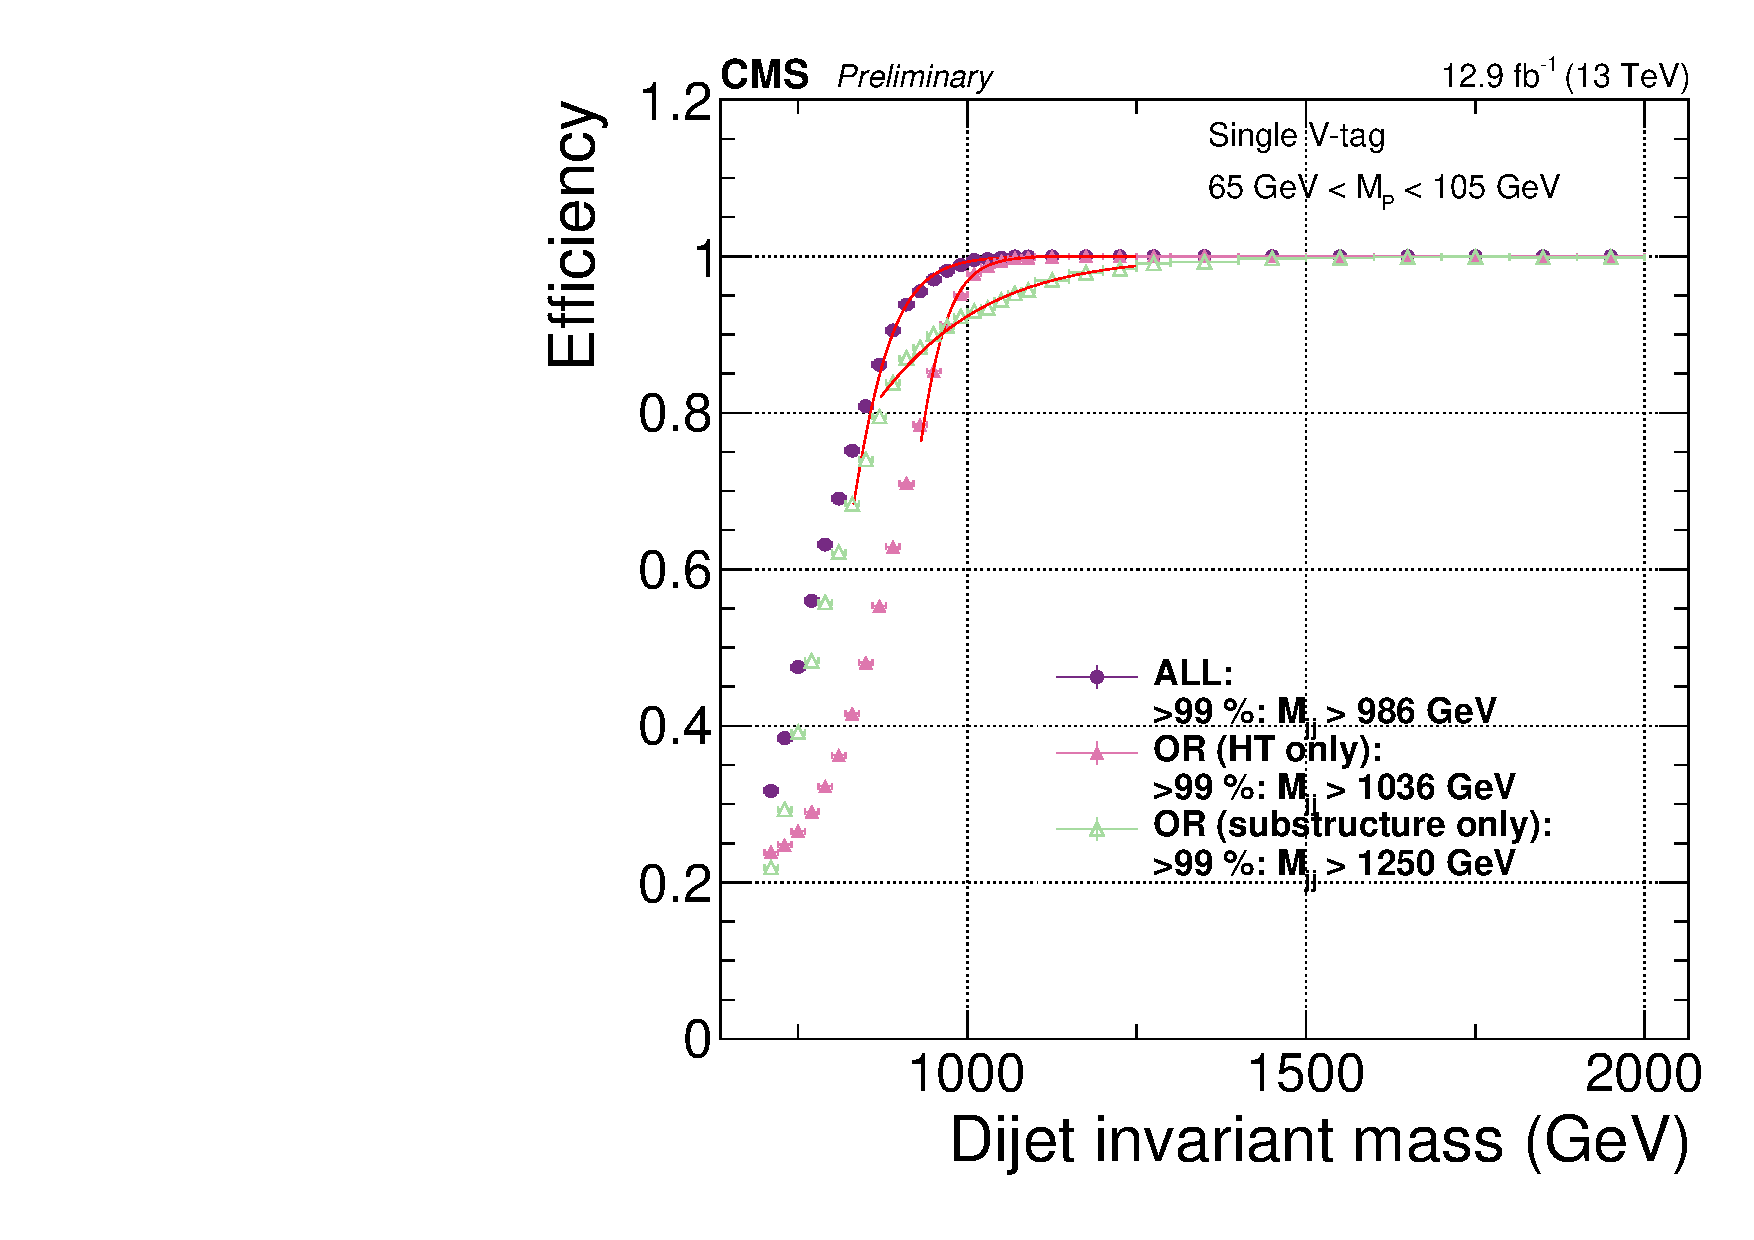
\includegraphics[width=0.49\textwidth]{figures/analysis/search2/AN-16-235/plots/triggereffMjj-ALL_SingleTag.pdf}
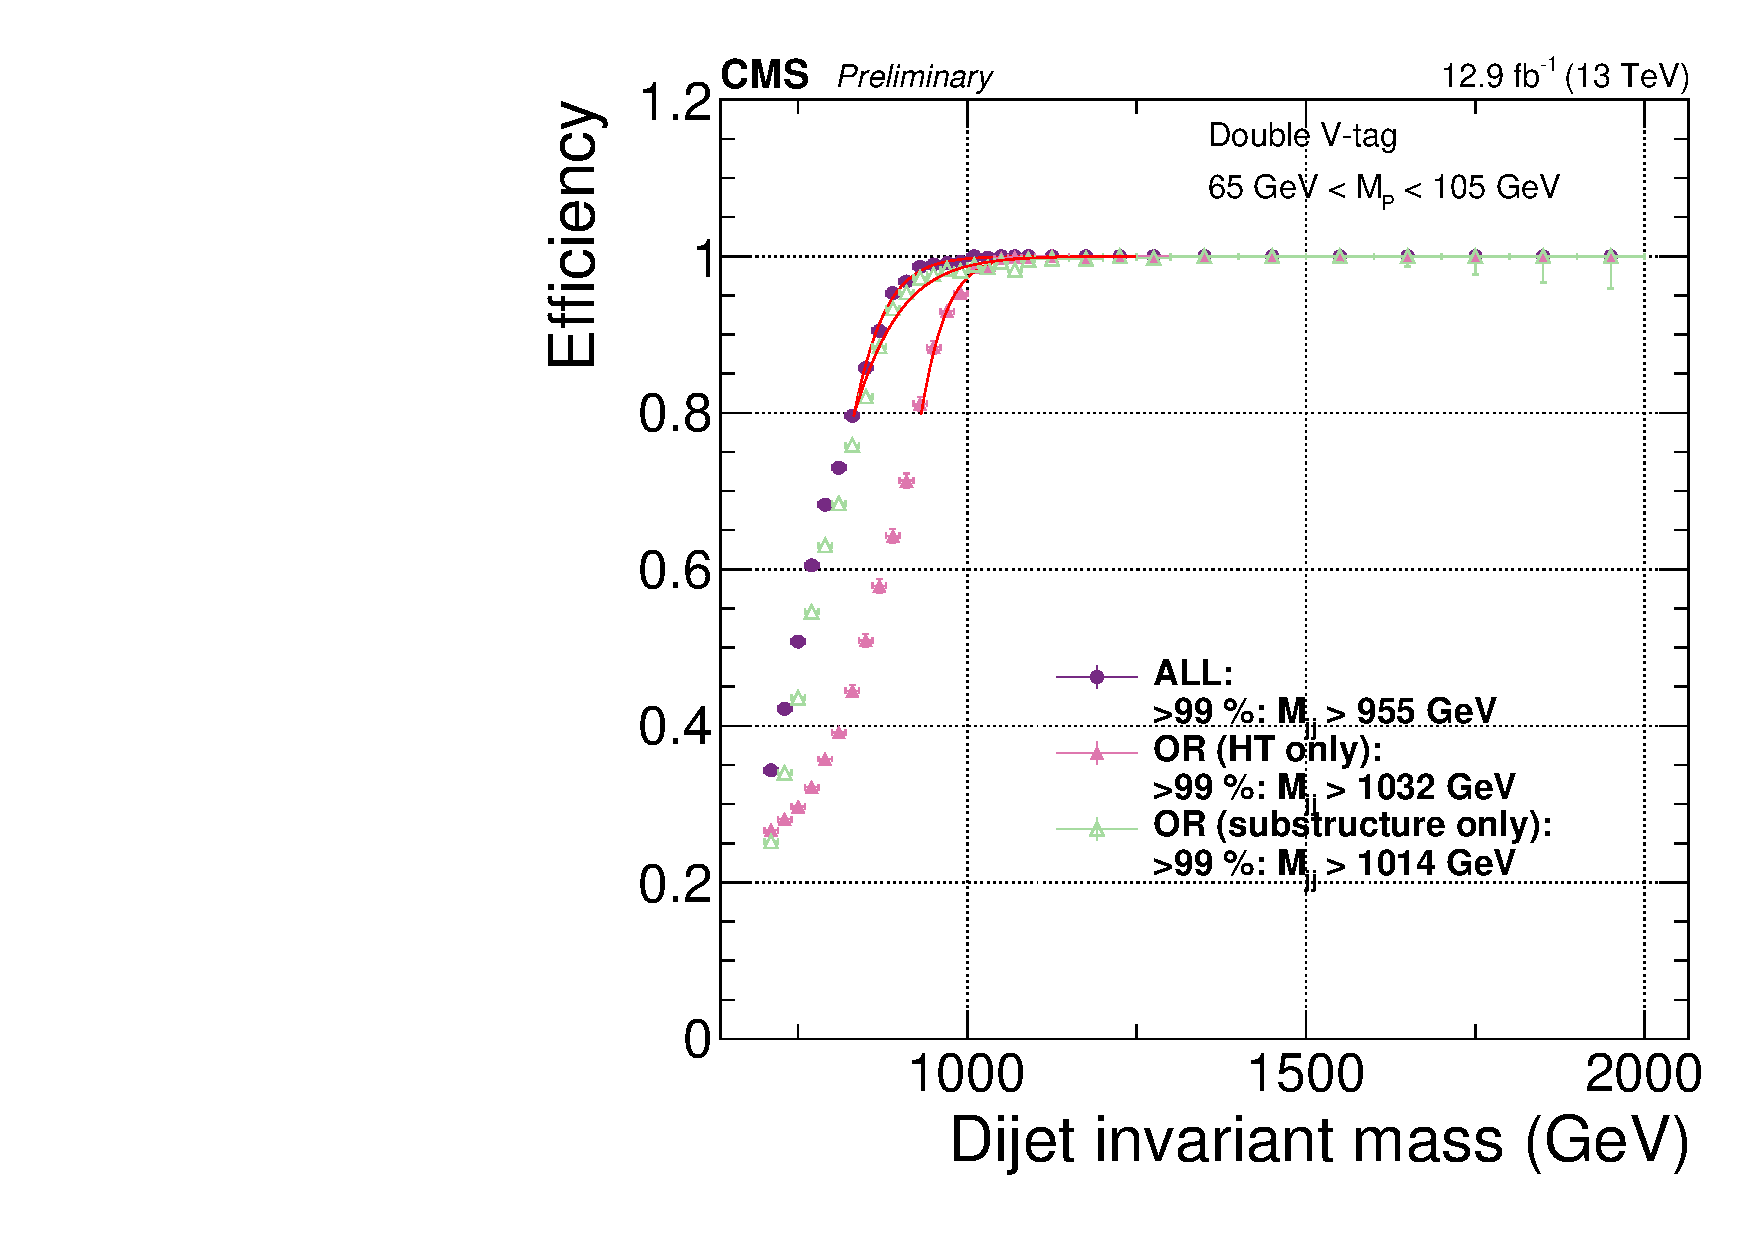
\includegraphics[width=0.49\textwidth]{figures/analysis/search2/AN-16-235/plots/triggereffMjj-ALL_DoubleTag.pdf}\\
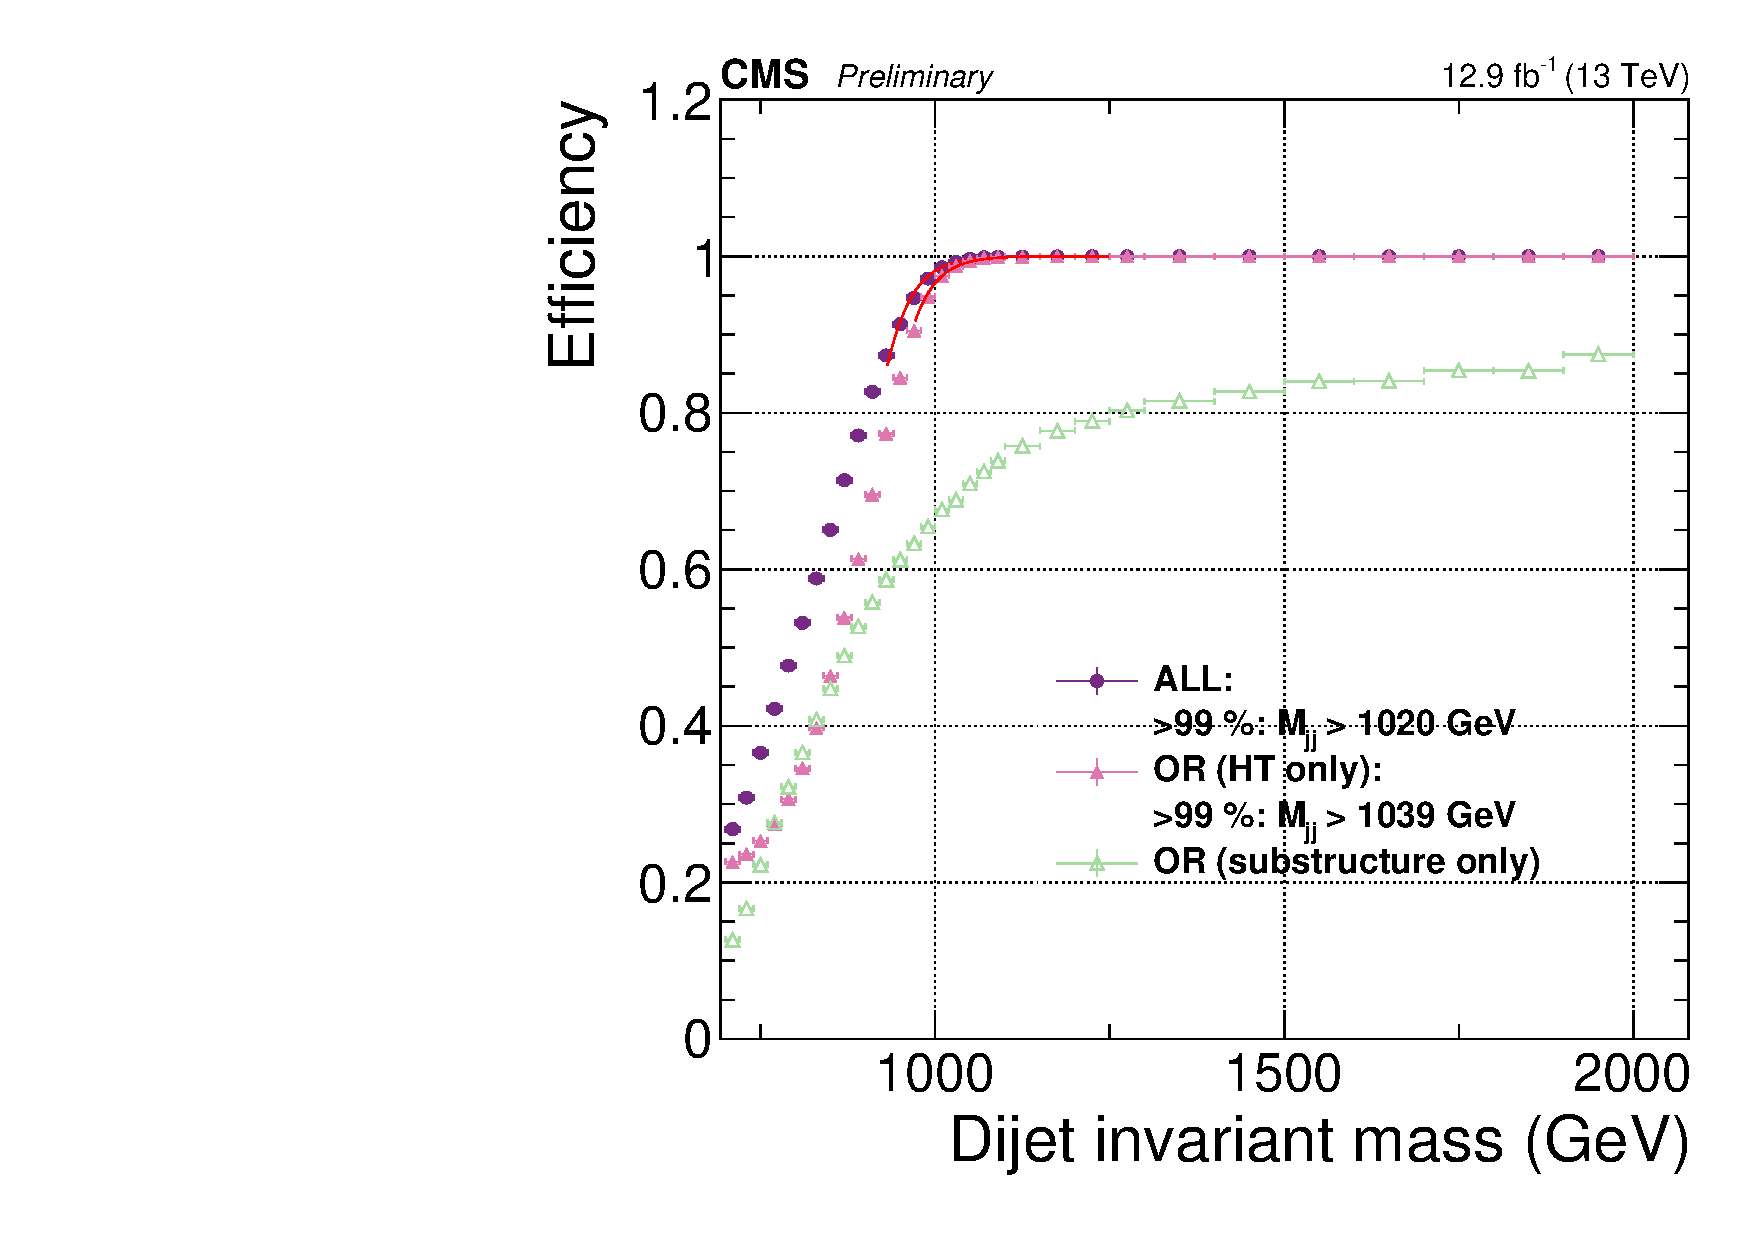
\includegraphics[width=0.49\textwidth]{figures/analysis/search2/AN-16-235/plots/triggereffMjj-ALL_noTag.pdf}

\caption{Comparison of trigger efficiencies for jets passing one of the HT-triggers only (pink), for jets passing one of the grooming-triggers only (green) and for jets passing one of the HT-triggers or one of the grooming triggers (purple). Here as a function of dijet invariant mass for all jet pairs passing loose selections and where one jet has a softdrop mass larger than 65 GeV (top left), both jets have a softdrop mass larger than 65 GeV (top right) and where no mass cut is applied (bottom). }
\label{fig:searchII:trigger-fits}
\end{figure}

Including grooming triggers lowers the 99\% trigger efficiency threshold by around 50(80) \GeV in the single (double) tag category once substructure is requested on the analysis level. Using the or of all triggers, we are safely on the trigger plateau for dijet invariant masses above 955(986) \GeV in the double (single) tag category, setting the analysis threshold at a dijet invariant mass of 955 \GeV for the double tag analysis and 990 \GeV for the single tag analysis. For controlplots, where no groomed mass window is applied, a trigger threshold of 1020 GeV is used.

\par Trigger efficiencies as a function of the offline softdrop-jet mass for the \\ 
\texttt{HLT\_AK8PFJet360\_TrimMass30} trigger are shown in Figure~\ref{fig:searchII:grooming-mj-trigger}. Here the jet transverse momentum of one of the jets is required to be at least 600 GeV and no other mass cut is applied. This trigger requires one jet to have a trimmed mass above 30 GeV at HLT level and reaches the trigger plateau for groomed-jet masses around 50 GeV. As reference trigger, the prescaled trigger \texttt{HLT\_PFJet320} is used. 
\begin{figure}[htb]
\centering
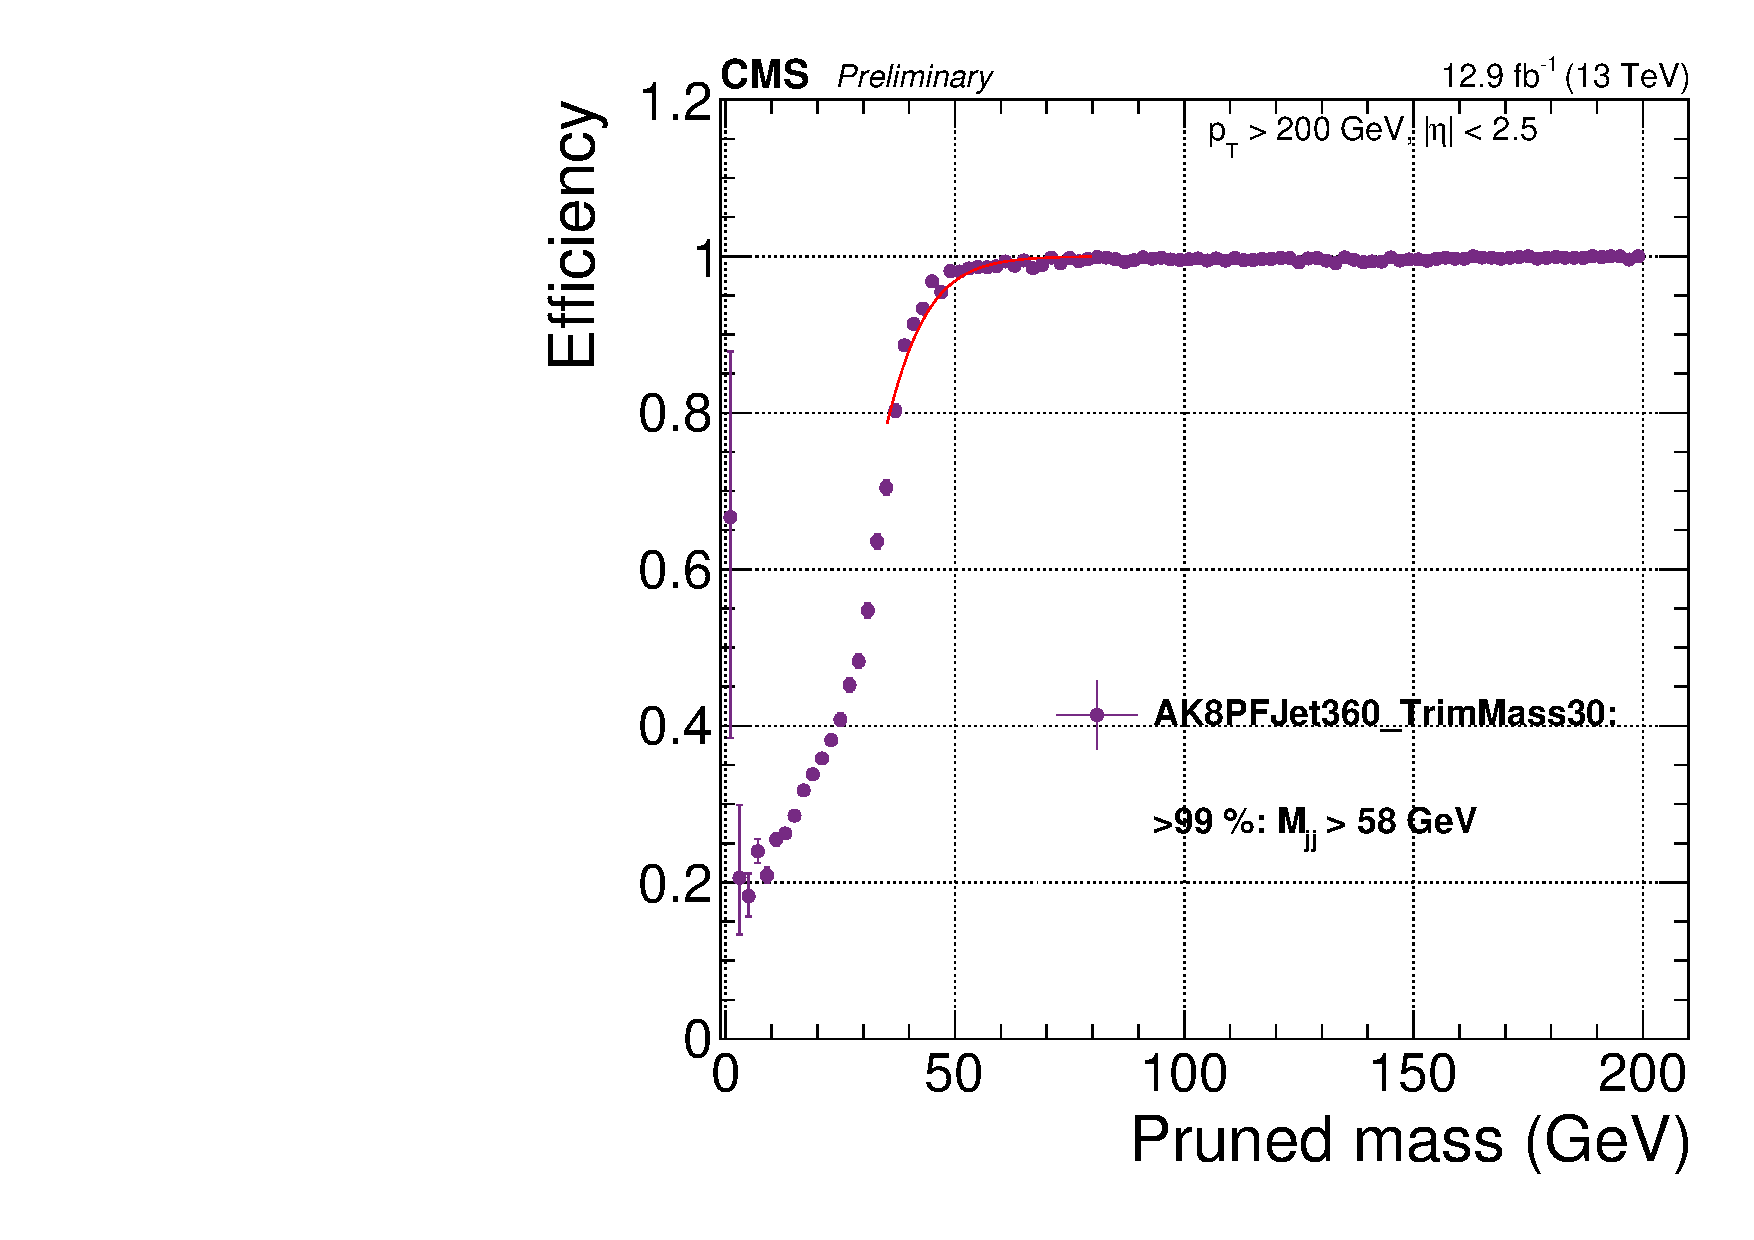
\includegraphics[width=0.49\textwidth]{figures/analysis/search2/AN-16-235/plots/triggereff-prunedmass_fit.pdf}
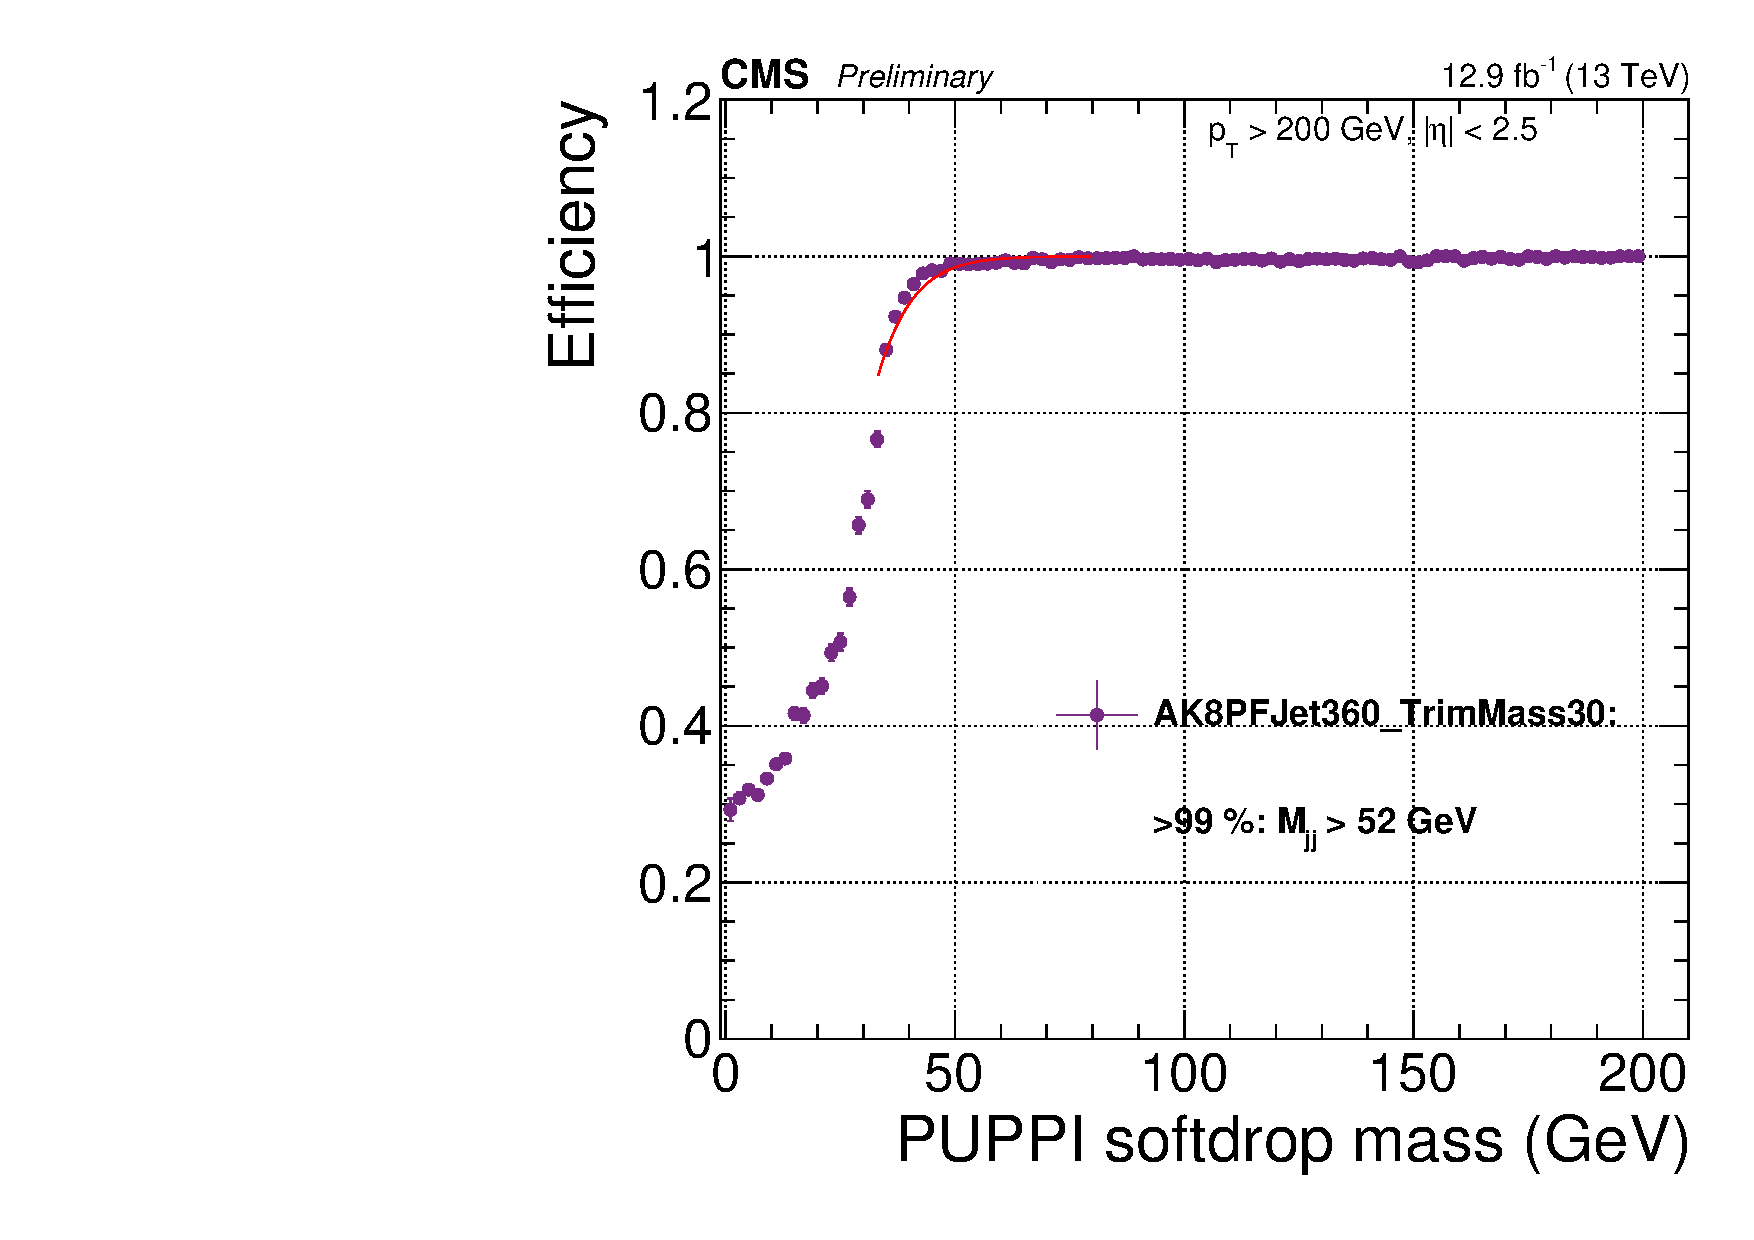
\includegraphics[width=0.49\textwidth]{figures/analysis/search2/AN-16-235/plots/triggereff-sdmass_fit.pdf}
\caption{Efficiency for the \texttt{HLT\_AK8PFJet360\_TrimMass30} trigger as a function of pruned-jet (left) and softdrop-jet (right) mass for jets with $\PT > \unit{600}{\GeV}$.}
\label{fig:searchII:grooming-mj-trigger}
\end{figure}

\subsubsection{Preselection}
The same preselections as in Search I, described in \label{sec:search1:preselection}, have been applied: We require two AK R=0.8 jets with CHS applied pre-clustering, required to pass the tight jet ID requirement, $\PT>200 \GeV$ and $|\eta|<2.5$. The same QCD t-channel suppressing cut of $|\Delta \eta|<1.3$ is required together with the following trigger thresholds on the dijet invariant mass: $\mjj > \unit{955} {\GeV}$ for the double V-tag and $\unit{990} {\GeV}$ for the single V-tag analysis. The jet \PT (top left), $\eta$ (top right), $\Delta \eta_{jj}$ and dijet invariant mass (bottom left) for the two leading jets in the event after loose preselections are applied is shown in Figure~\ref{fig:searchII:kinematics-all}.

\begin{figure}[h!]
\centering
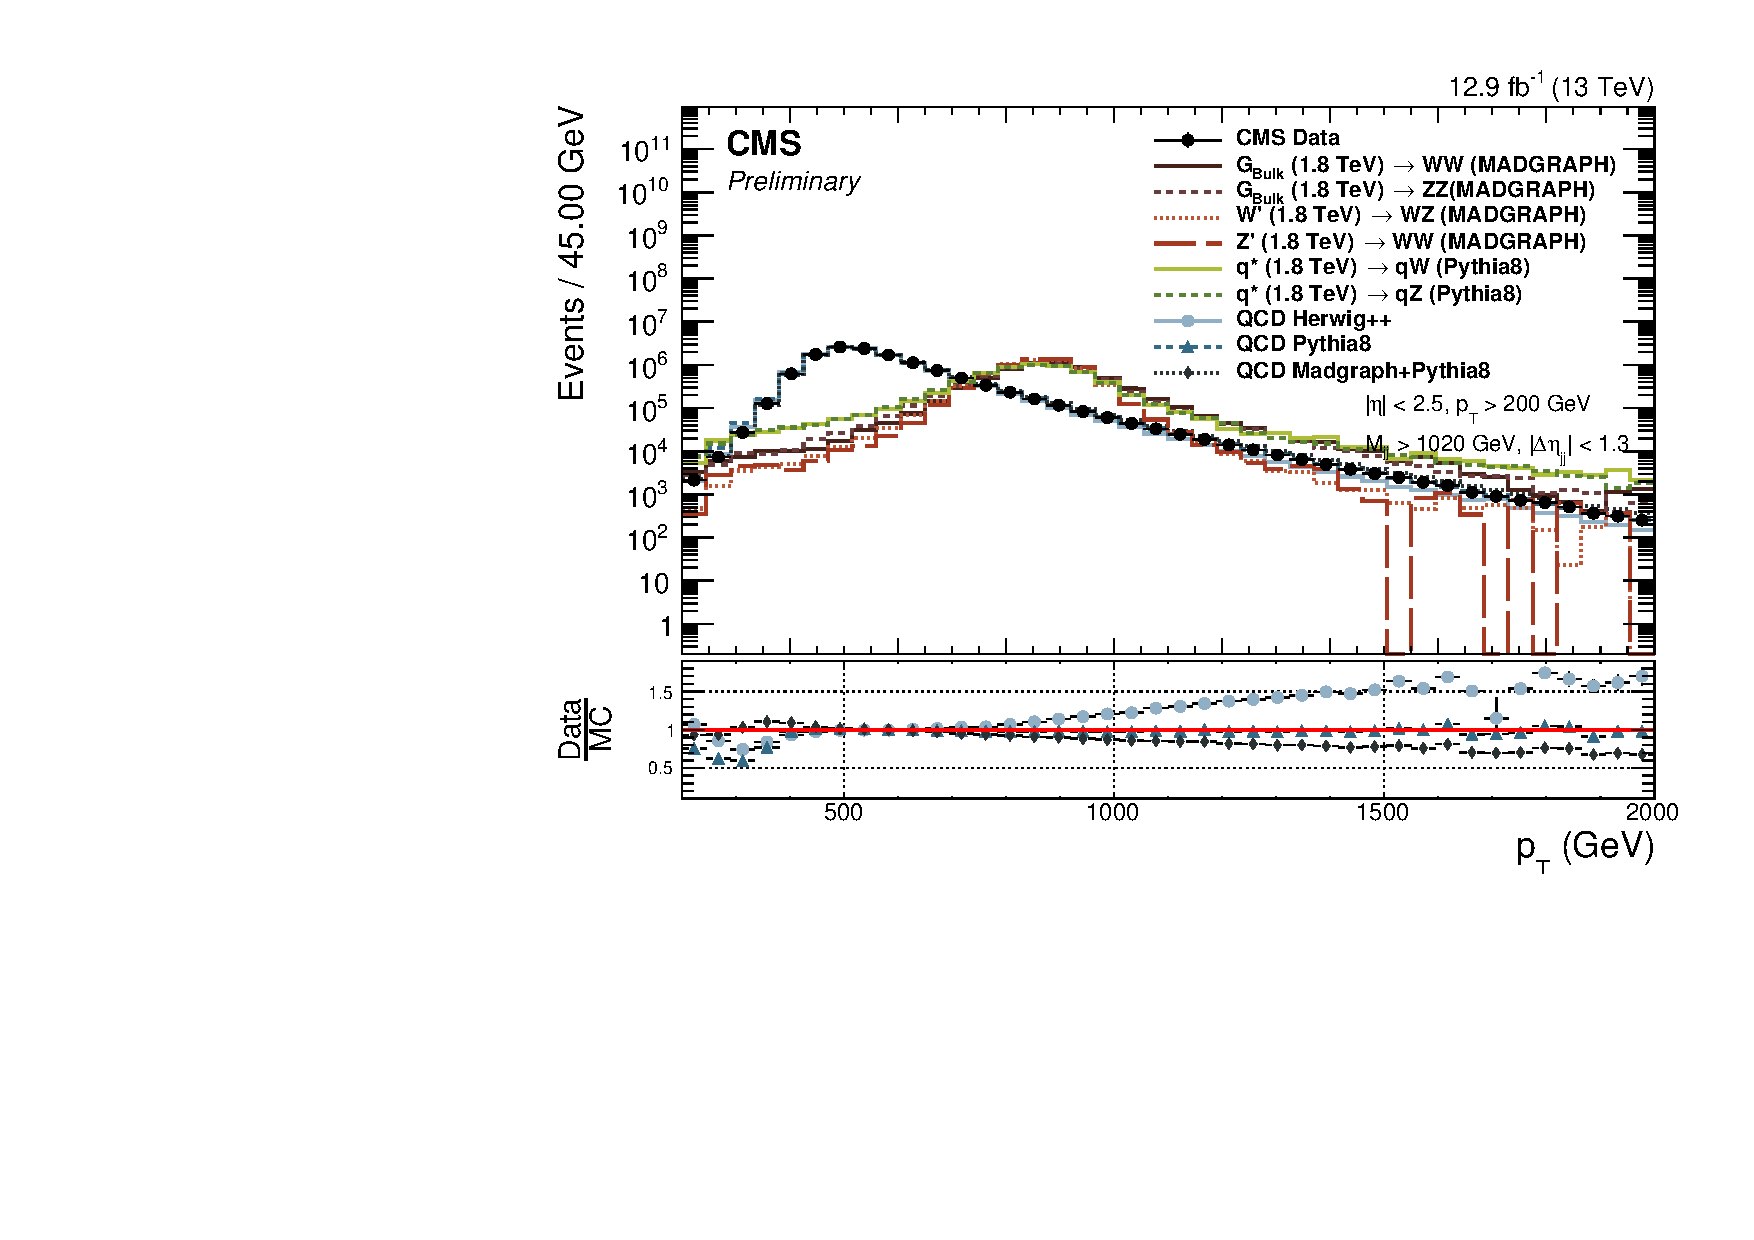
\includegraphics[width=0.49\textwidth]{figures/analysis/search2/AN-16-235/plots/qcdcp_Pt.pdf}
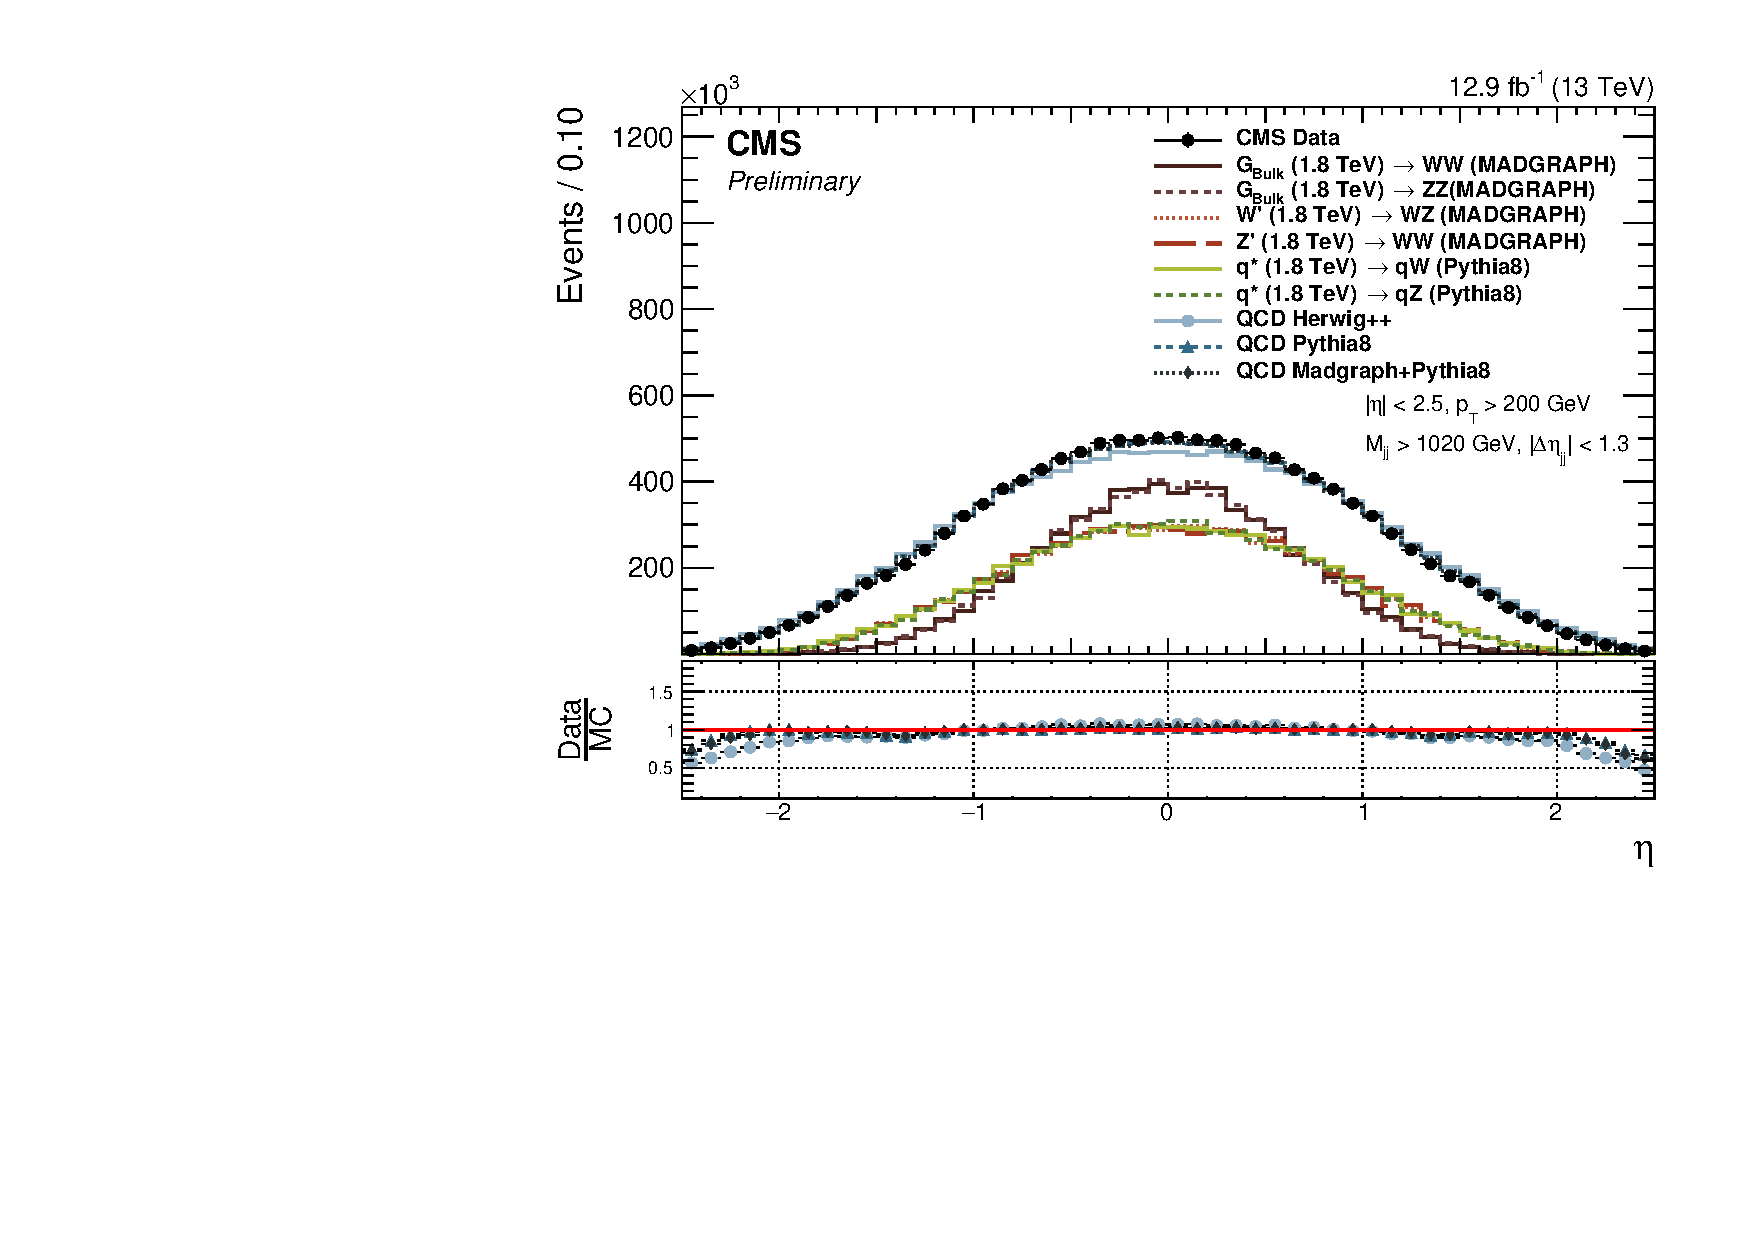
\includegraphics[width=0.49\textwidth]{figures/analysis/search2/AN-16-235/plots/qcdcp_Eta.pdf}\\
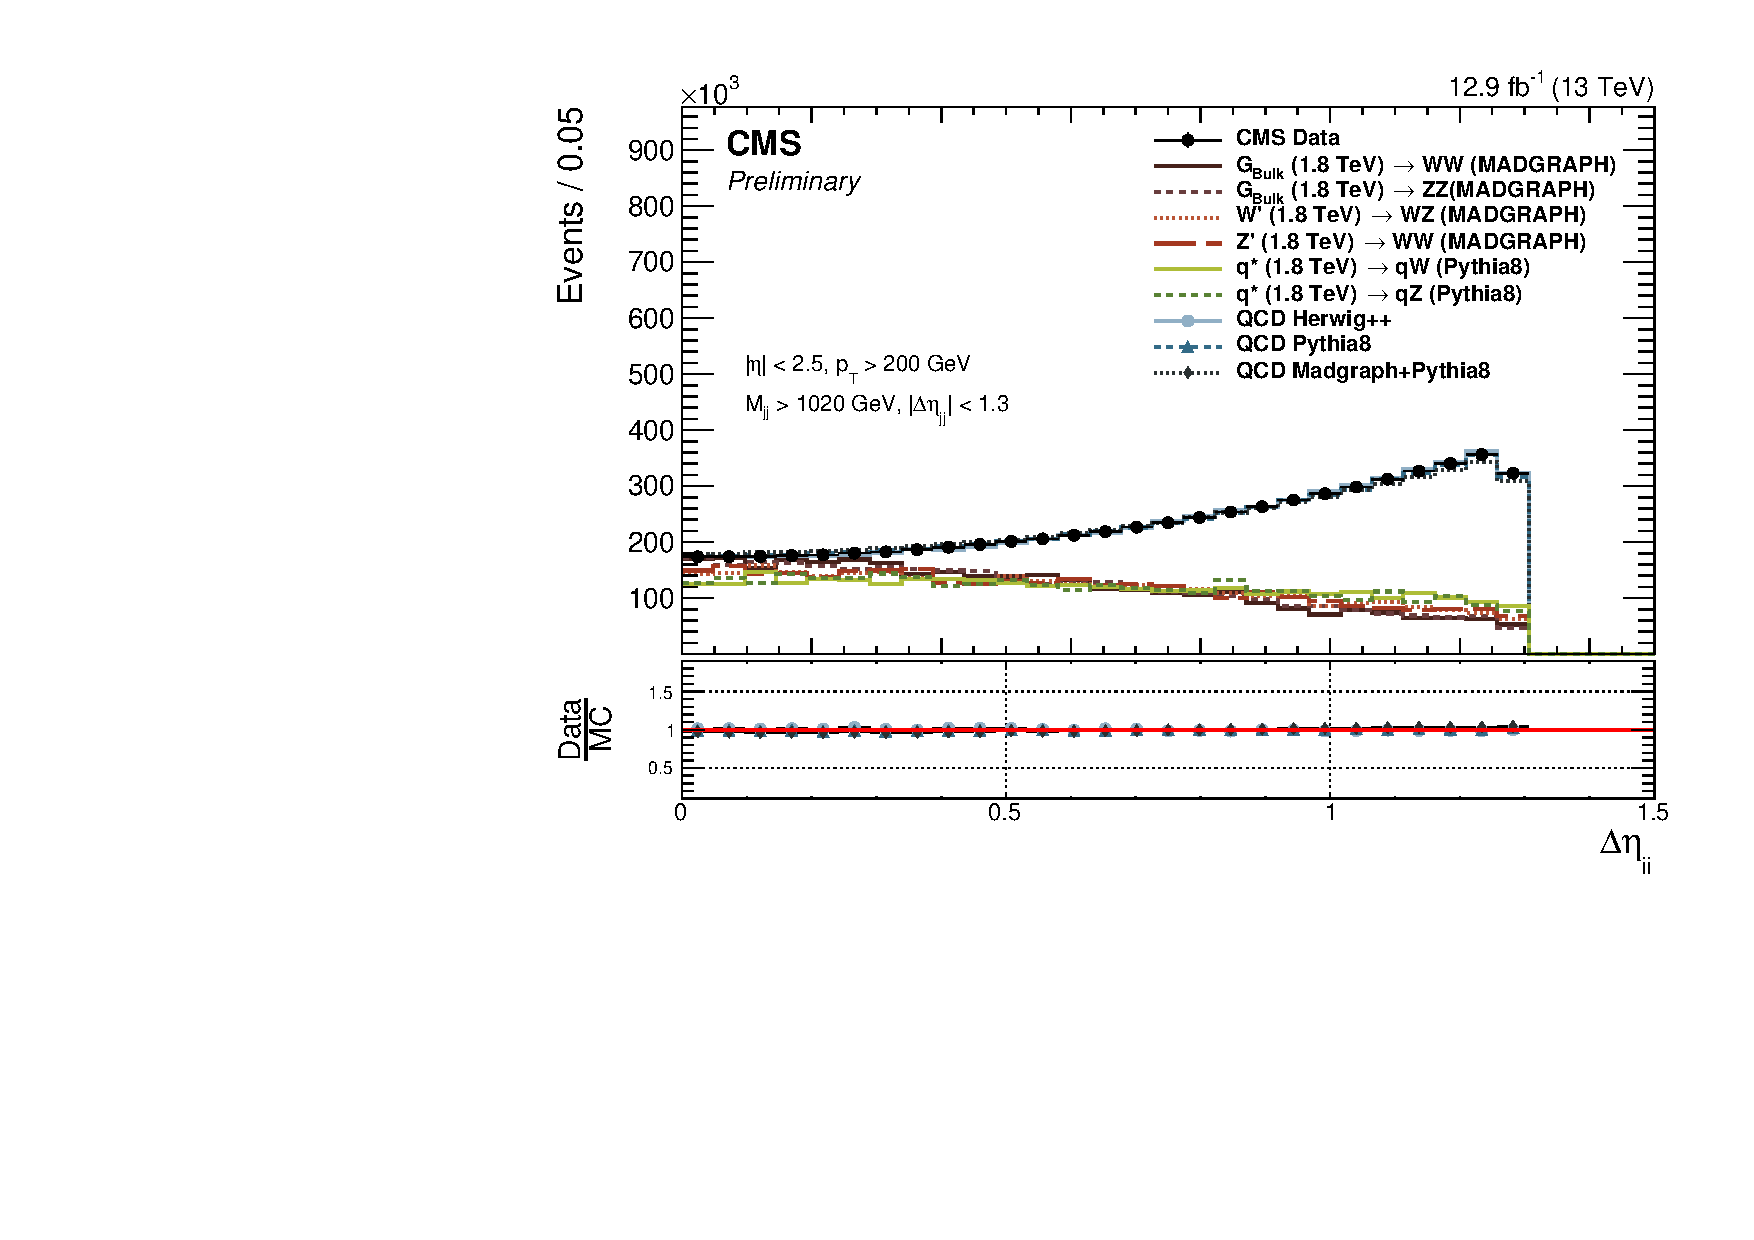
\includegraphics[width=0.49\textwidth]{figures/analysis/search2/AN-16-235/plots/qcdcp_DeltaEta.pdf}
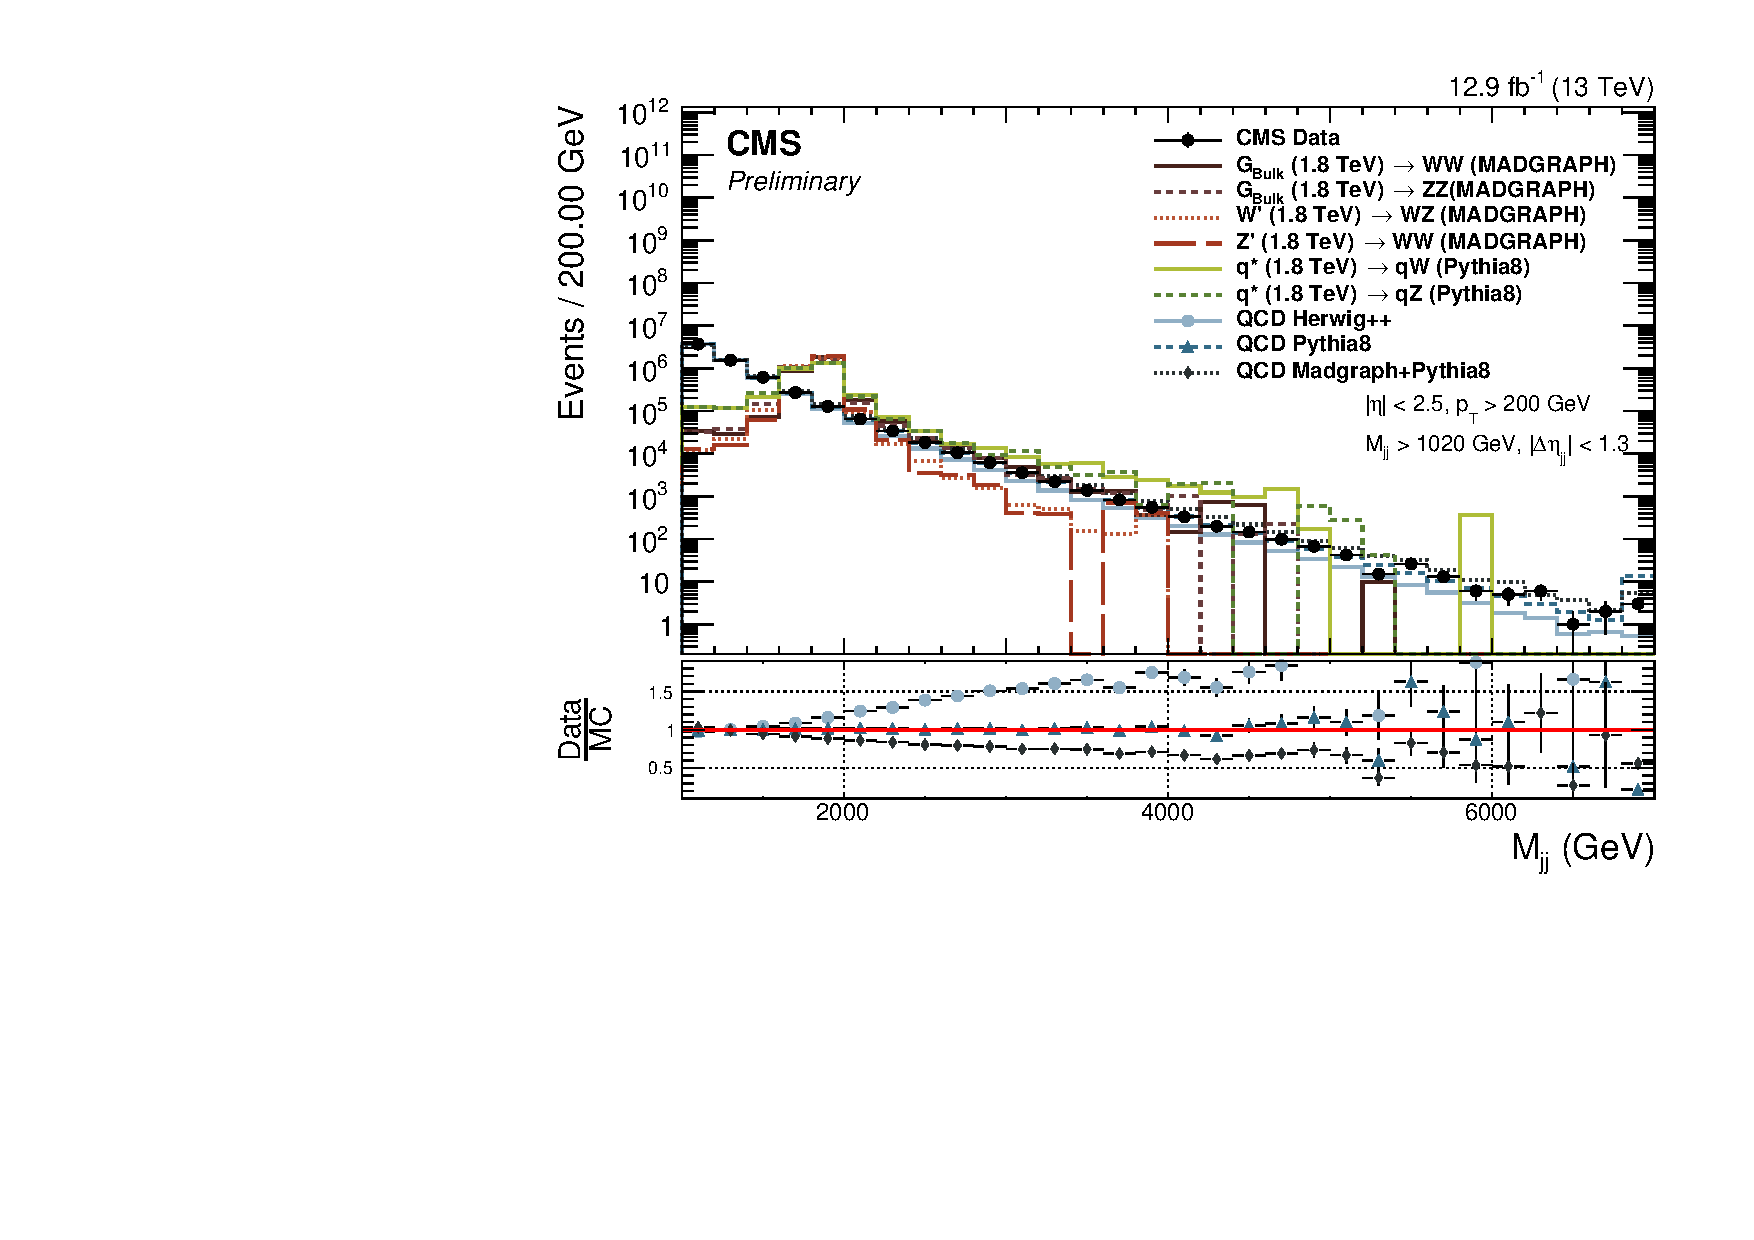
\includegraphics[width=0.49\textwidth]{figures/analysis/search2/AN-16-235/plots/qcdcp_Mjj.pdf}
\caption{Jet \PT{} (top left), $\eta$ (top right), $\Delta \eta_{jj}$ and dijet invariant mass (bottom left) for the two leading jets in the event after loose preselections are applied. The signal is scaled by an arbitrary number.}
\label{fig:searchII:kinematics-all}
\end{figure}

A large difference in slope in the jet \PT and dijet invariant mass spectrum depending on the QCD matrix element or shower generator is observed. Pure \PYTHIA QCD MC describes the data best, while \HERWIG{++} and \amcatnlo{}+\PYTHIA tend to under- or over-estimate the number of high $\PT/\mjj$ jets, respectively. Pure \PYTHIA QCD MC is therefore used for all background checks in this analysis.


\subsection{Developing a new W-tagger}
\label{sec:searchII:puppisoftdrop}
As mentioned in the introduction to this chapter, early studies had shown that the PUPPI pileup subtraction algorithm yielded superior resolution on large-cone jet observables like the jet mass. We therefore wanted to check whether the softdrop jet mass, and its observed sensitivity to the Underlying Event and pileup, would be improved if a better pileup subtraction algorithm was applied pre-clustering.\par
Two interesting observations were made. Softdrop used together with PUPPI pileup subtraction displayed a much smaller \PT-dependent shift than CHS+Softdrop, as hoped. Figure~\ref{fig:searchII:sdmass} shows the PUPPI softdrop mass for W-jets from a 1 \TeV ($\PT\sim 500 \GeV$) and 4 \TeV ($\PT\sim 2 \TeV$) resonance, exhibiting the desired reduced \PT dependence in jet mass scale. 

\begin{figure}[htb]
\centering
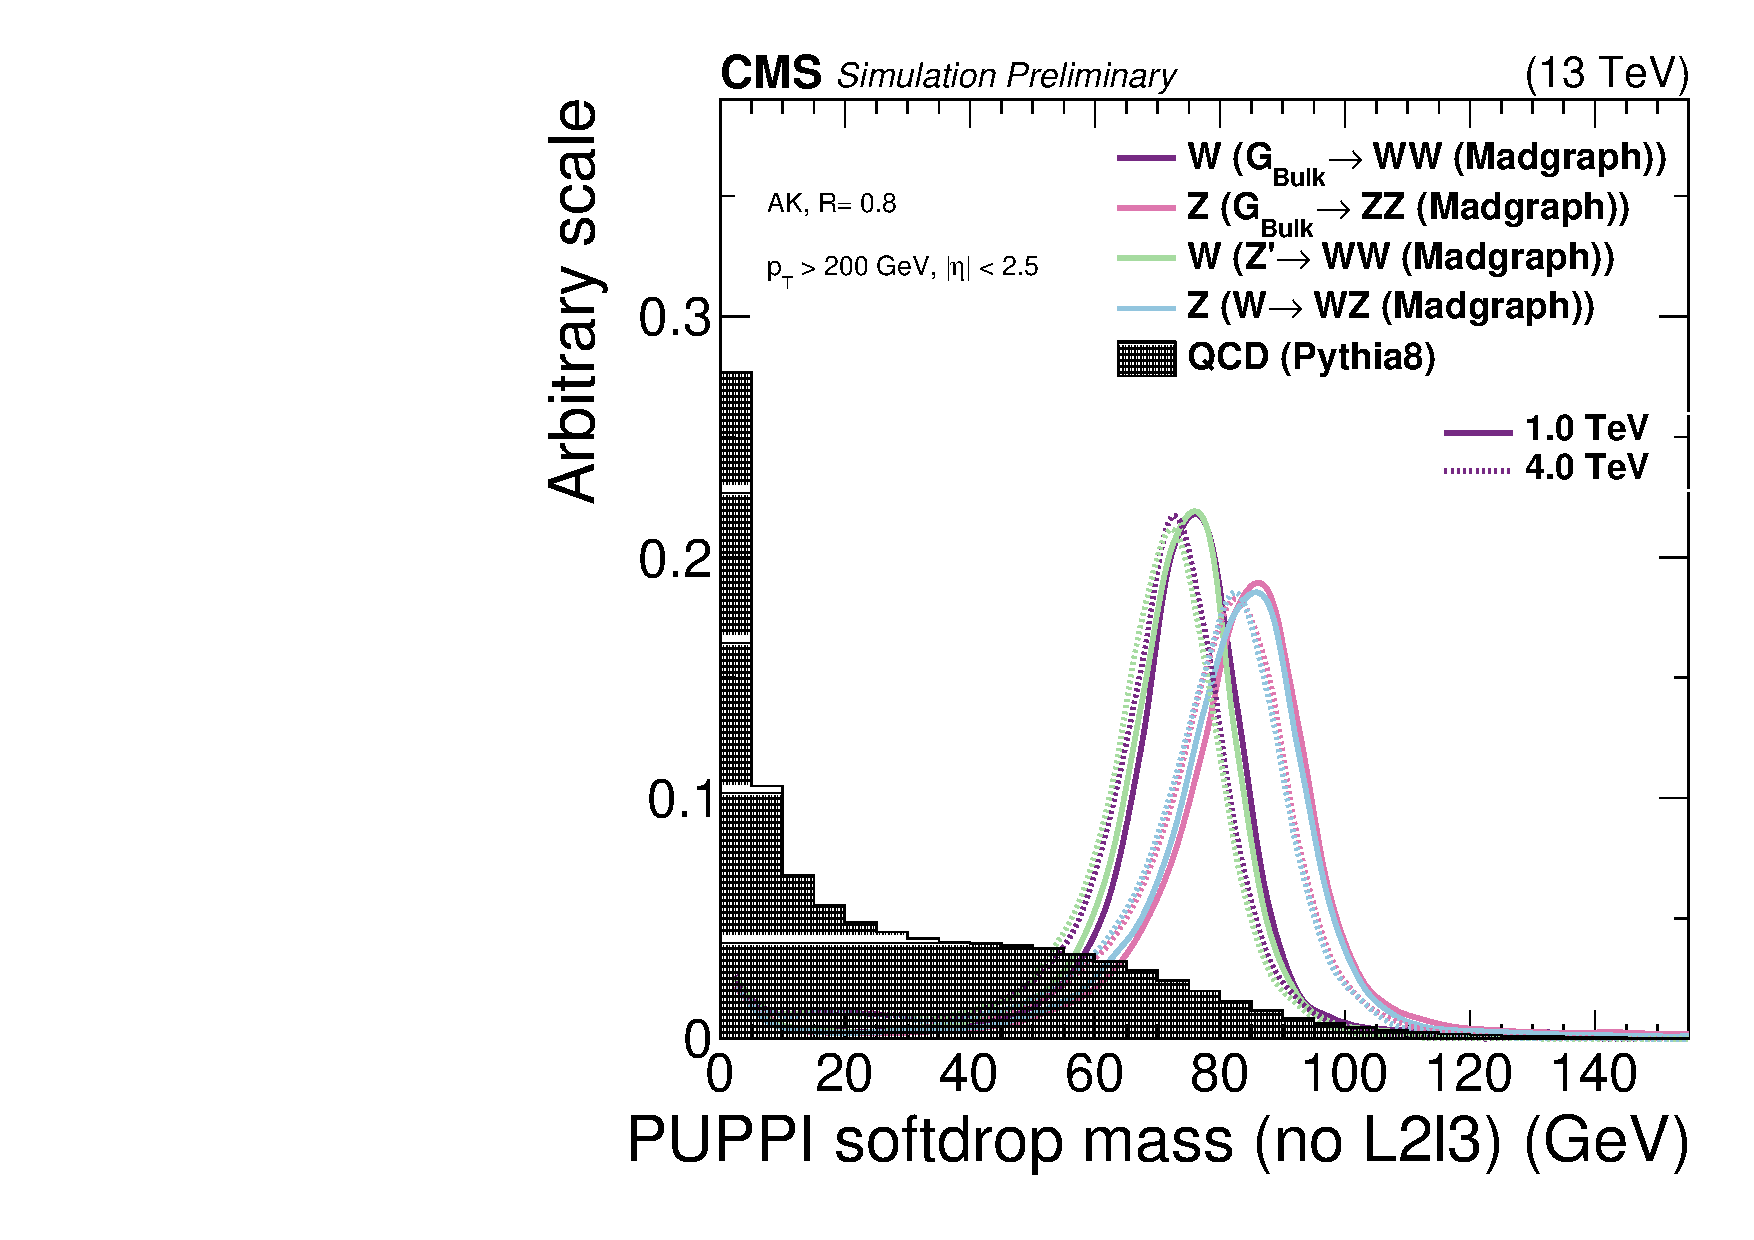
\includegraphics[width=0.49\textwidth]{figures/analysis/search2/AN-16-235/plots/gen_SoftdropMassUnCorr.pdf}
\caption{The  PUPPI softdrop jet mass distribution with no jet energy corrections applied}
\label{fig:searchII:sdmass}
\end{figure}

However, when applying centrally provided L2 and L3 jet energy corrections (see Section~\ref{sec:objreco:jec}) to the jet groomed mass, as is recommended, a strong \PT dependence is re-introduced. This effect is not present for the pruned jet mass. Figure~\ref{fig:searchII:wtagmass} show the softdrop (top left) and pruned (top right) jet mass distribution with recommended L2L3 corrections applied. Here, the PUPPI+softdrop jet mass shift is significantly increased with respect to what was observed for the uncorrected mass, while CHS+pruned jet mass is stable. This points to the PUPPI jet energy corrections not being optimal for scalar jet mass variables, while they may be good for correcting jet 4-vectors. The jet energy corrections derived for CHS and PUPPI jets as a function of jet \PT is shown in the bottom plot in Figure~\ref{fig:searchII:wtagmass} . A significant slope in JEC as a function of \PT is measured for PUPPI, while not present for CHS.

\begin{figure}[htb]
\centering
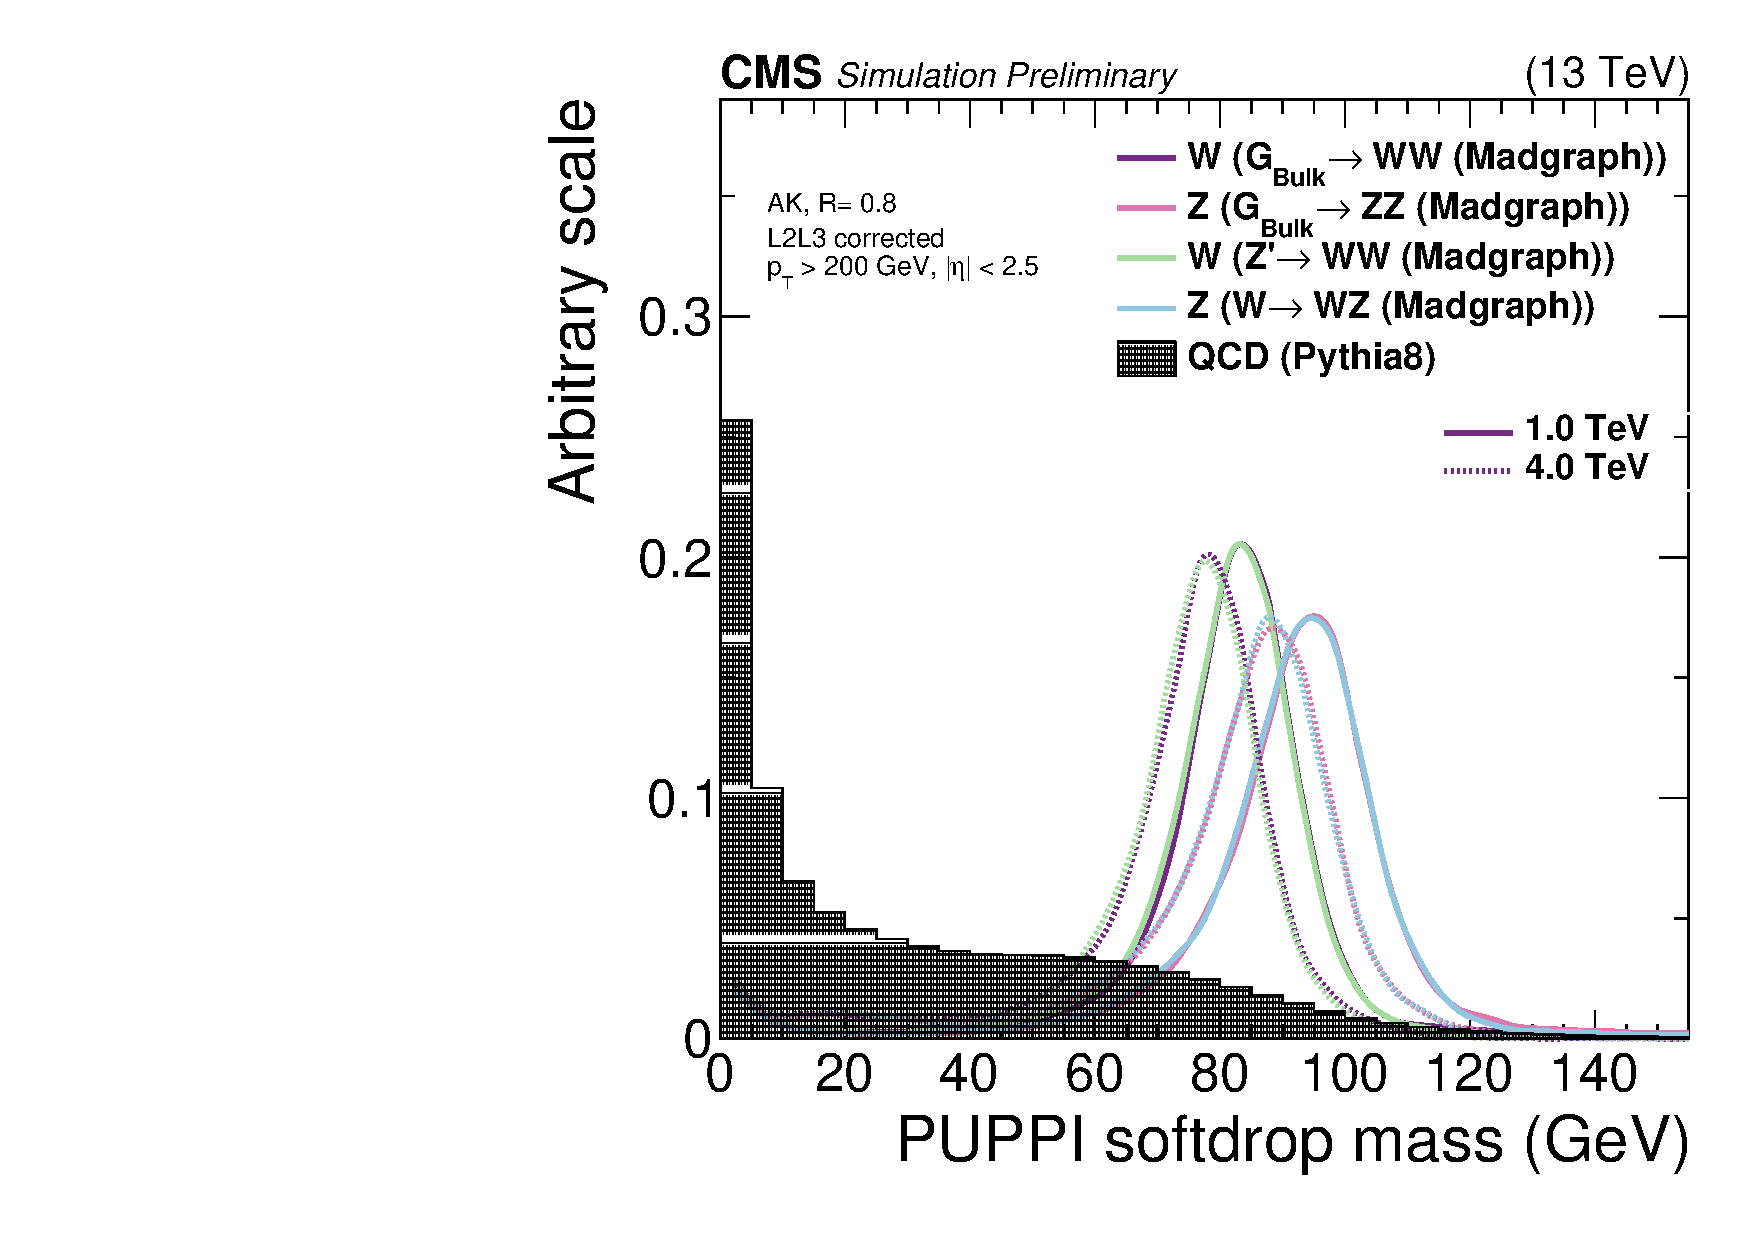
\includegraphics[width=0.49\textwidth]{figures/analysis/search2/AN-16-235/plots/gen_SoftdropMass.pdf}
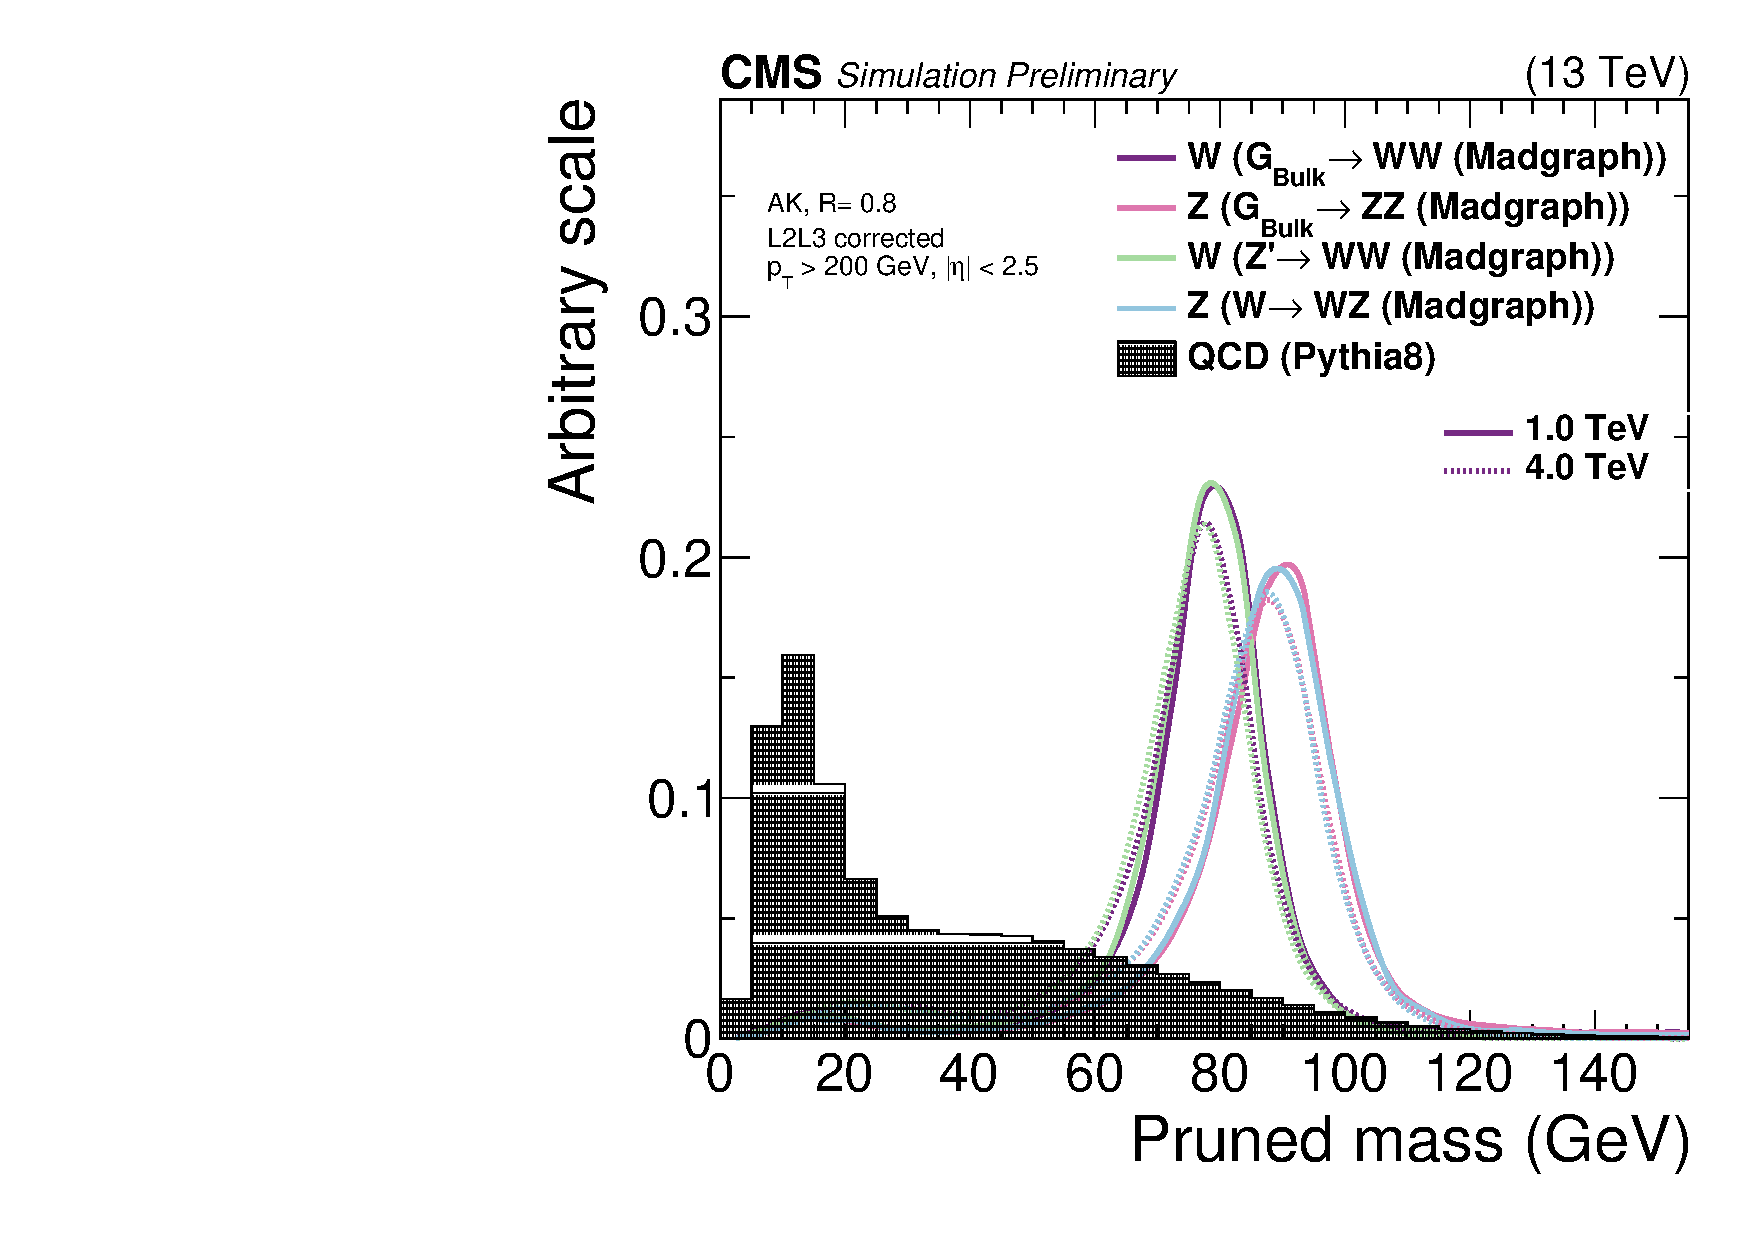
\includegraphics[width=0.49\textwidth]{figures/analysis/search2/AN-16-235/plots/gen_PrunedMass.pdf}\\
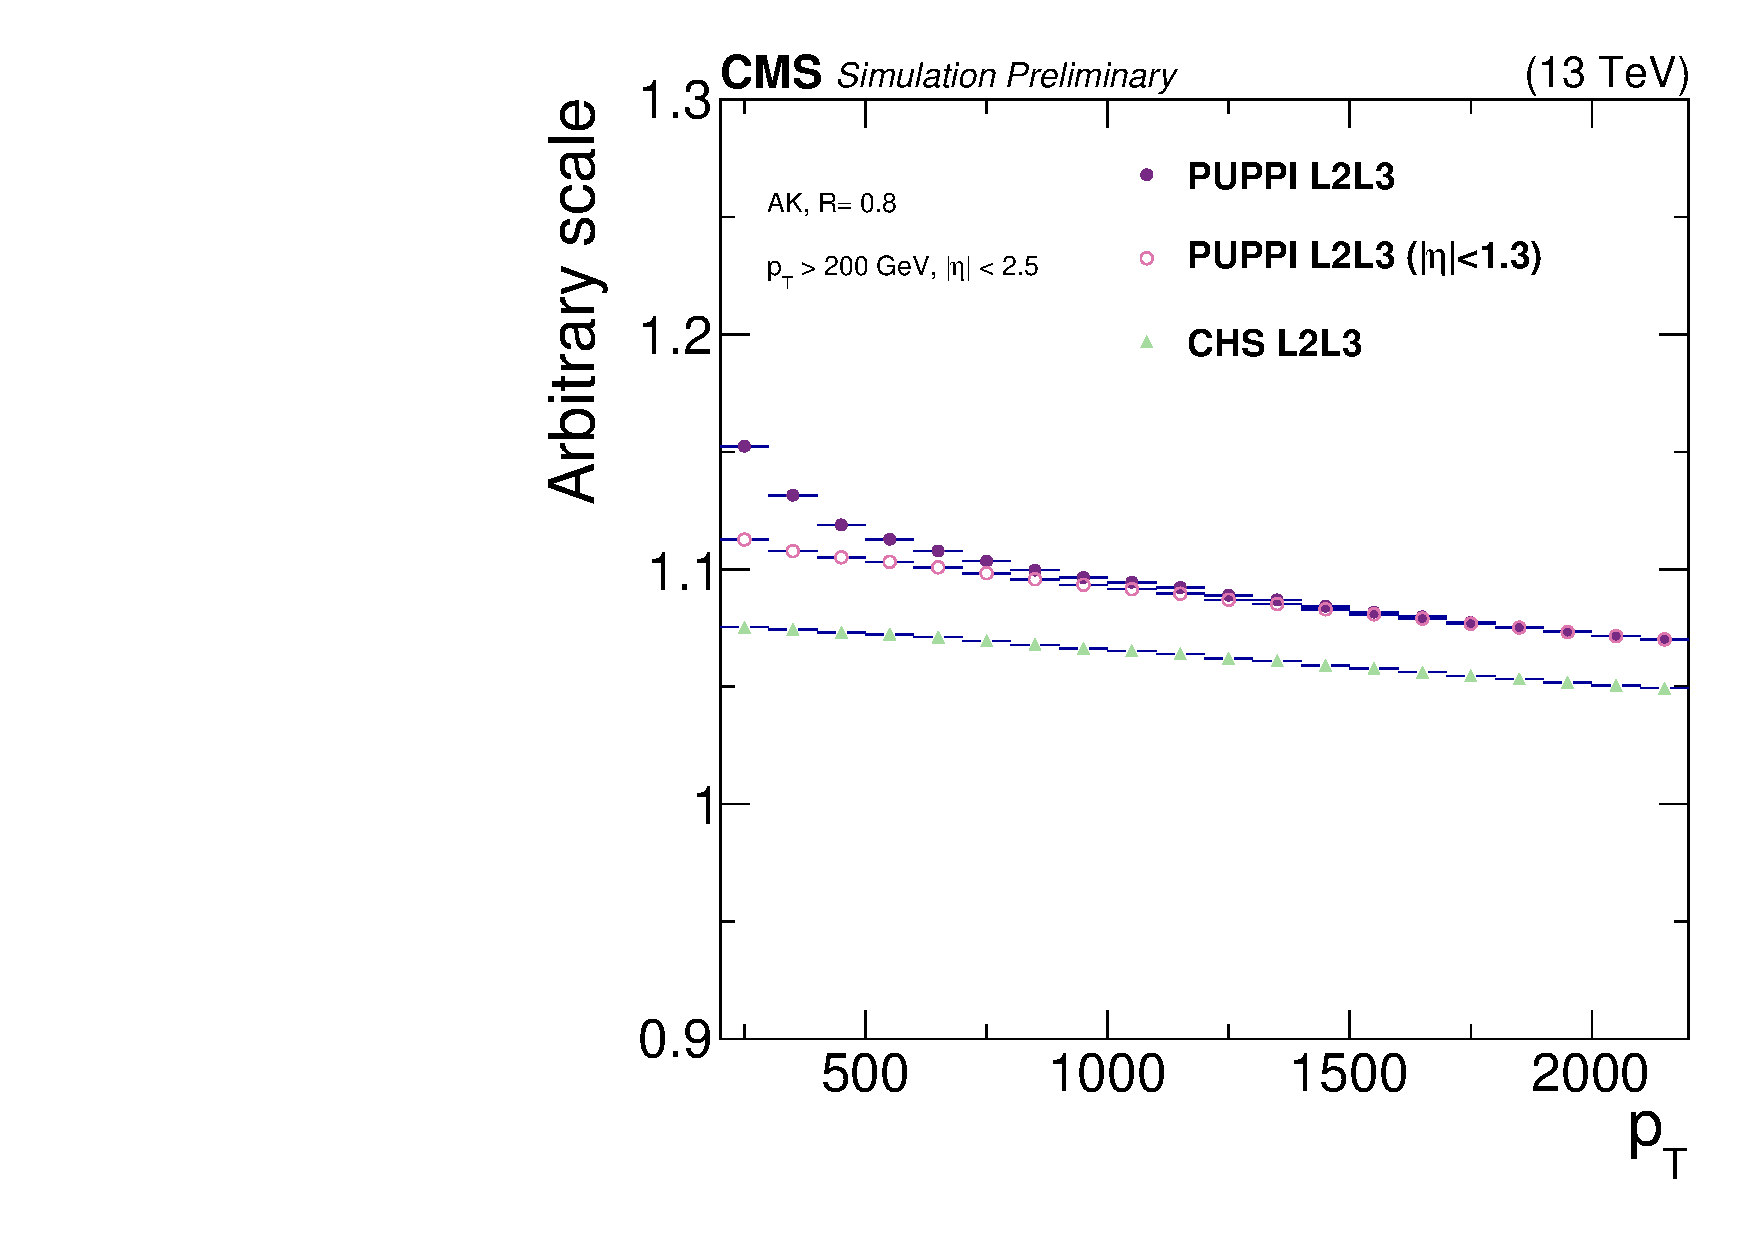
\includegraphics[width=0.49\textwidth]{figures/analysis/search2/AN-16-235/plots/JECvsPT.pdf}
\caption{Top: PUPPI softdrop mass distribution (top left) and pruned jet mass distribution (top right) with L2 and L3 corrections applied. Bottom: The projection of CHS and PUPPI jet energy corrections versus jet \PT.}
\label{fig:searchII:wtagmass}
\end{figure}

\subsection{Dedicated PUPPI+softdrop mass corrections}

In order to minimize \PT dependence in the PUPPI softdrop jet mass, all jet energy corrections to the softdrop jet mass are removed. However, this still leaves a residual \PT dependence and, in addition, the uncorrected mass does not peak at the correct W-mass of 80.4~\GeV. Figure~\ref{fig:searchII:UncorrSD} shows the mean of a Gaussian fit to the uncorrected PUPPI softdrop mass as a function of jet $\pt$ in two different $\eta$ bins (smaller or greater than $|\eta|=1.3$) for W-jets coming from a Bulk Graviton signal sample. A mass shift both as a function of $\eta$ and \PT is observed, together with an average mean significantly lower than the W-mass.

\begin{figure}[htbp]
\centering
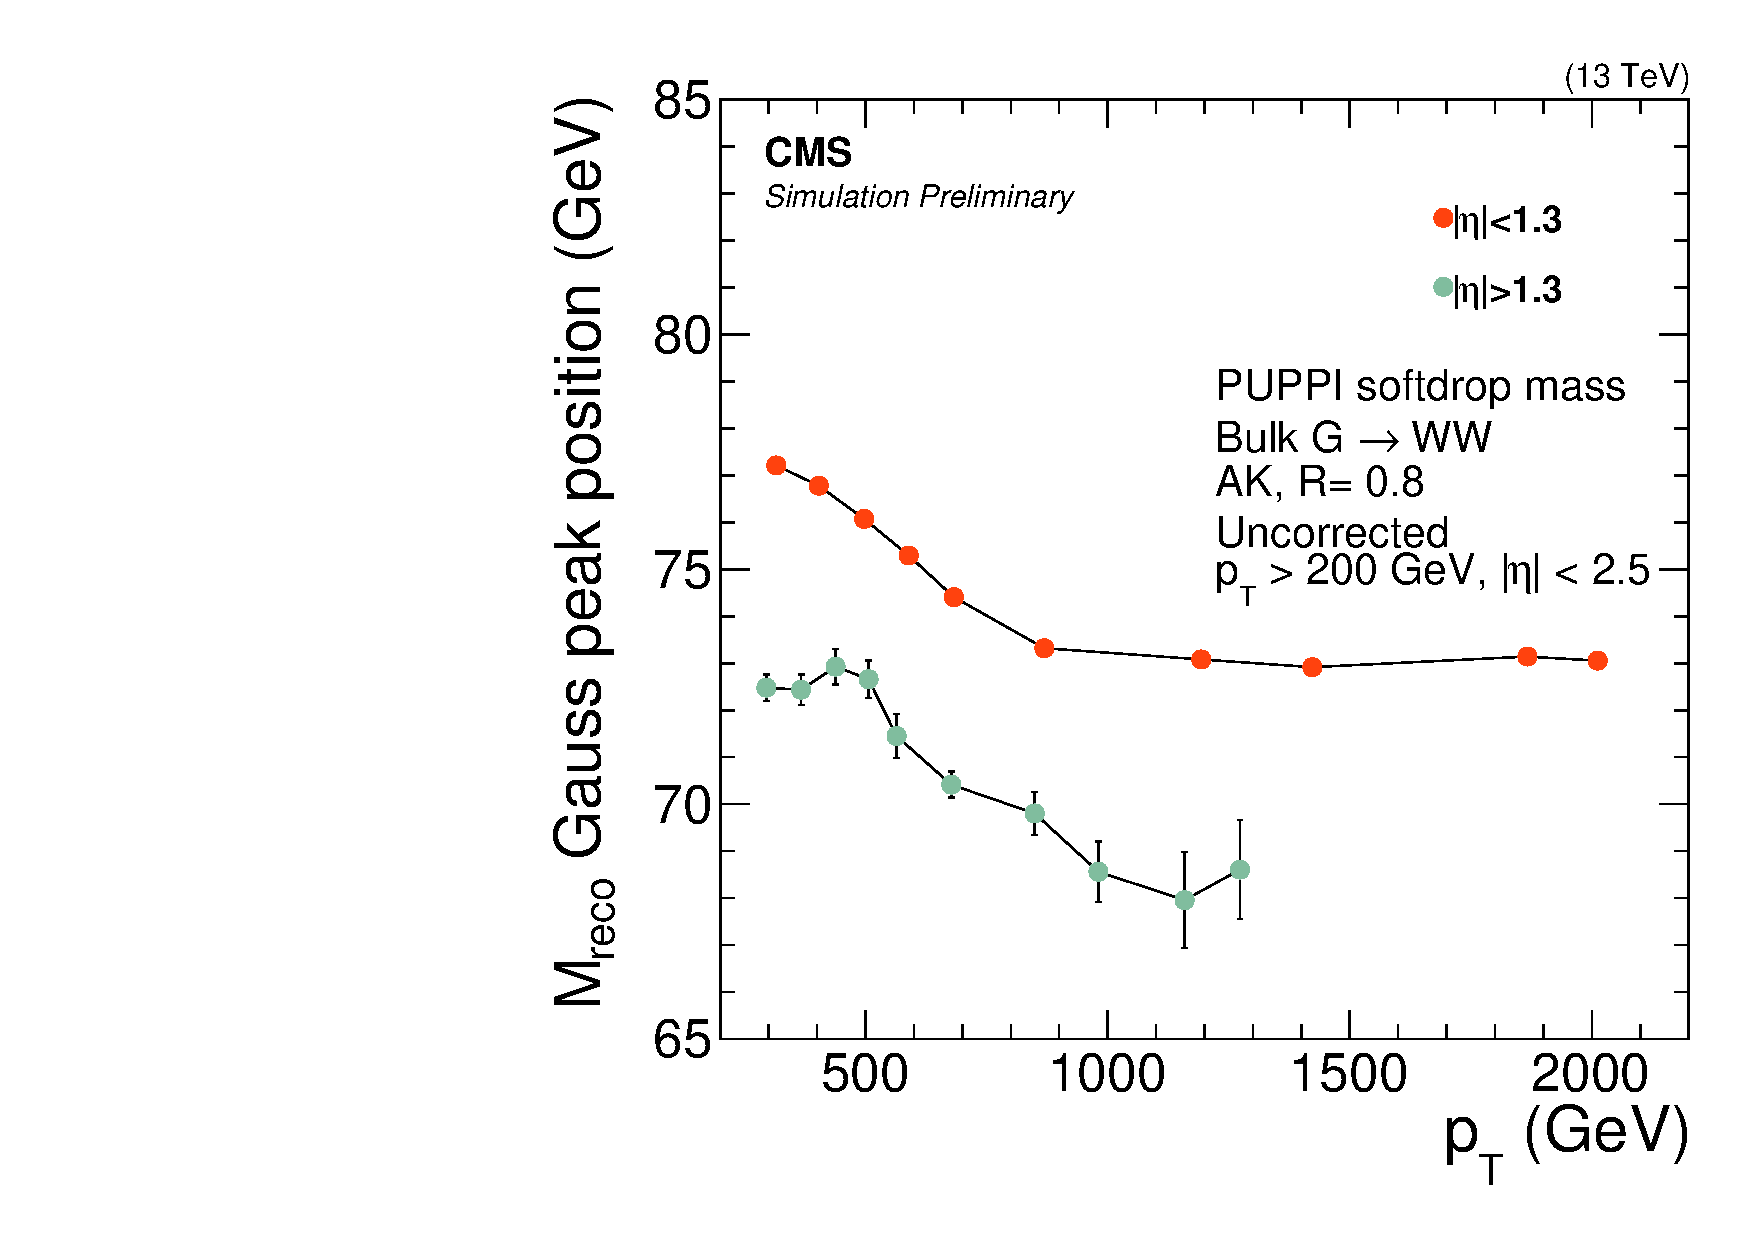
\includegraphics[width=0.49\textwidth]{figures/analysis/search2/AN-16-235/plots/RecoPuppiSoftdropMass_vspt.pdf}
\caption{The mean of a Gaussian fit to the W-jet PUPPI softdrop mass peak as a function of jet \PT in two different $\eta$ bins (smaller or greater than $|\eta|=1.3$). No corrections have been applied to the softdrop mass.}
\label{fig:searchII:UncorrSD}
\end{figure}

In order to use PUPPI+softdrop for W-tagging, we therefore derive dedicated jet mass corrections to compensate for two factors: A generator level \PT-dependence, as first observed in \label{sec:searchI:wtagging}, and a reconstruction level \PT- and $\eta$-dependence, most likely caused by UE effects and the growing effective sofdrop radius at low jet \PT. Figure~\ref{fig:searchII:sdmassshifts} shows the mean of the generated softdrop mass (left) and the normalized difference in reconstructed and generated softdrop mass (right) as a function of jet \PT. The shift in generated softdrop mass at lower \PT is of the order of 2-3$\%$ while the difference between reconstructed and generated softdrop mass is a 5-10$\%$ effect.

\begin{figure}[htbp]
\centering
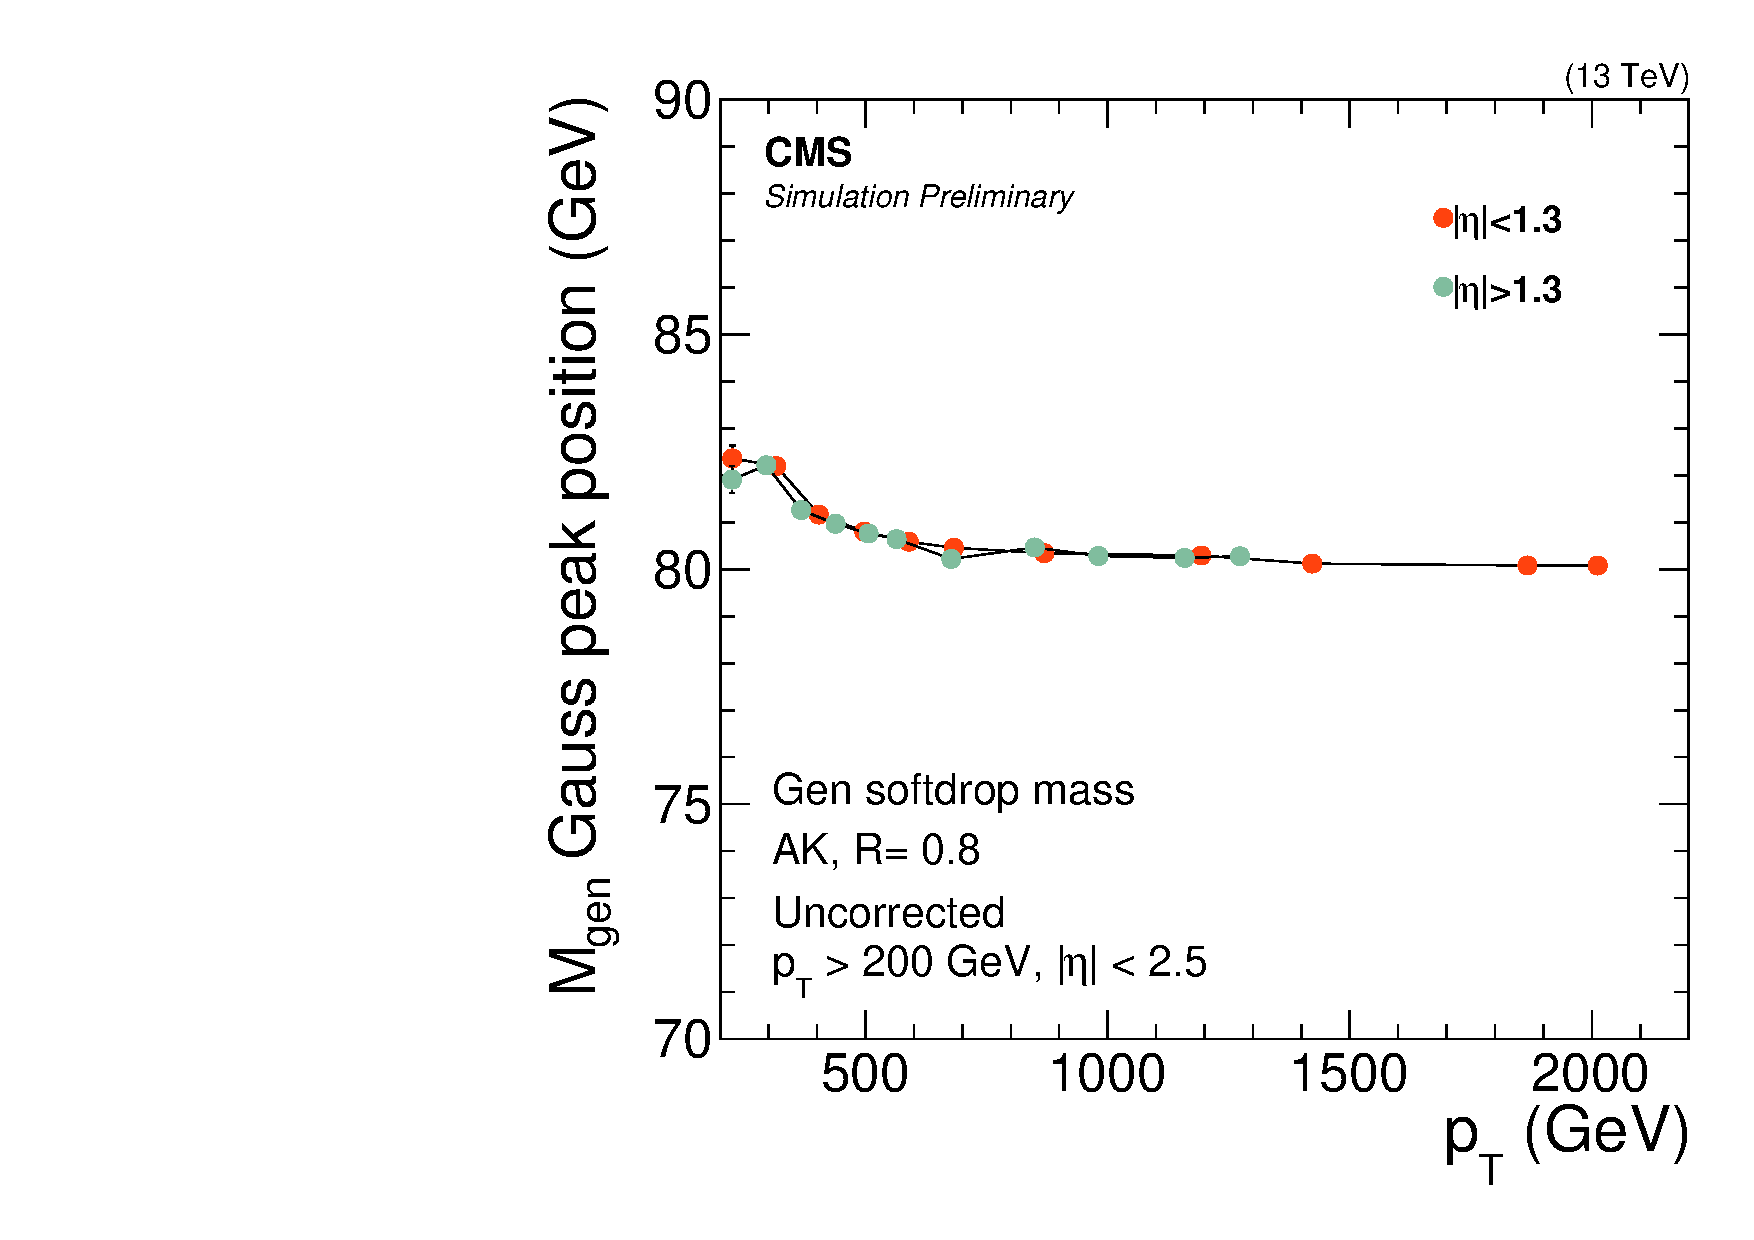
\includegraphics[width=0.49\textwidth]{figures/analysis/search2/AN-16-235/plots/GenSoftdropMass_vspt.pdf}
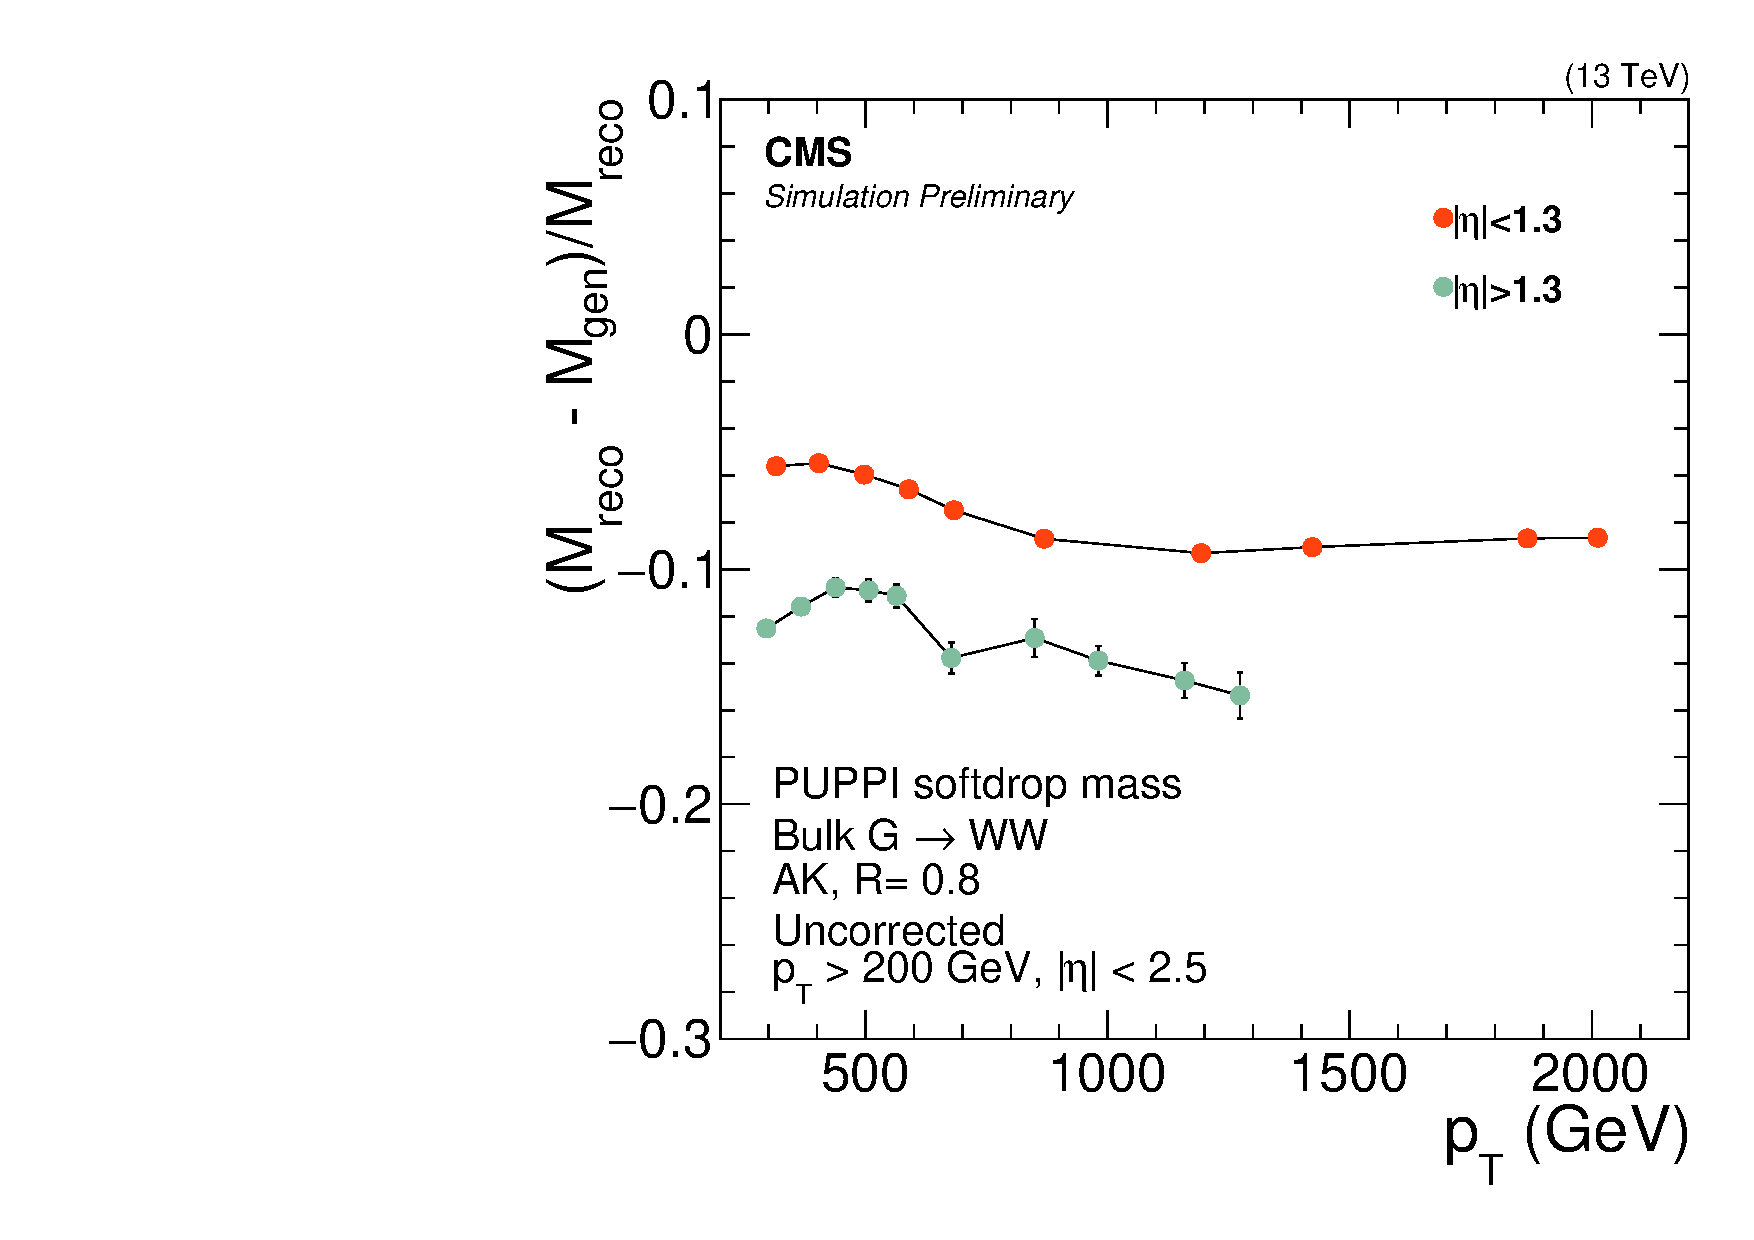
\includegraphics[width=0.49\textwidth]{figures/analysis/search2/AN-16-235/plots/MassShift_vspt.pdf}
\caption{The mean of the fitted generator level W-jet softdrop mass distribution as a function of jet $\pt$ (left) and the normalized difference in reconstructed and generated softdrop mass (right).}
\label{fig:searchII:sdmassshifts}
\end{figure}

The mass shift introduced at generator level is corrected by a fit to $\rm{M_{PDG}/M_{GEN}}$ as a function of jet \PT, where $\rm{M_{PDG}}=80.4~\GeV$ and $\rm{M_{GEN}}$ is the fitted mean of the generator level mass as shown in the left plot in Figure~\ref{fig:searchII:sdmassshifts}. To correct for the residual shift between generated and reconstructed softdrop mass, a fit to $\rm{(M_{RECO}-M_{GEN})/M_{RECO}}$, where $\rm{M_{RECO}}$ is the reconstructed mass shown in the right plot in Figure~\ref{fig:searchII:sdmassshifts} and $\rm{M_{GEN}}$ is as defined above, as a function of jet \PT in two $\eta$ bins (smaller or greater than $|\eta|=1.3$) is performed.
Polynomial fit functions of the following forms are used
\begin{align*} 
% w(\pt) &=  [0]+[1]*pow(x*[2],-[3] \\
w(\pt) &=  A  +B(x^{2})^{-C}          &\sim\textrm{"gen correction"}\\ 
w(\pt) &=  A  +Bx+Cx^2+Dx^3+Ex^4+Fx^5 &\sim\textrm{"reco correction"} 
\end{align*}

The distribution and corresponding fits for the two weights is shown in Figure~\ref{fig:jmcfits} for the "gen correction" (left) and "reco correction" (right).
\begin{figure}[htbp]
\centering
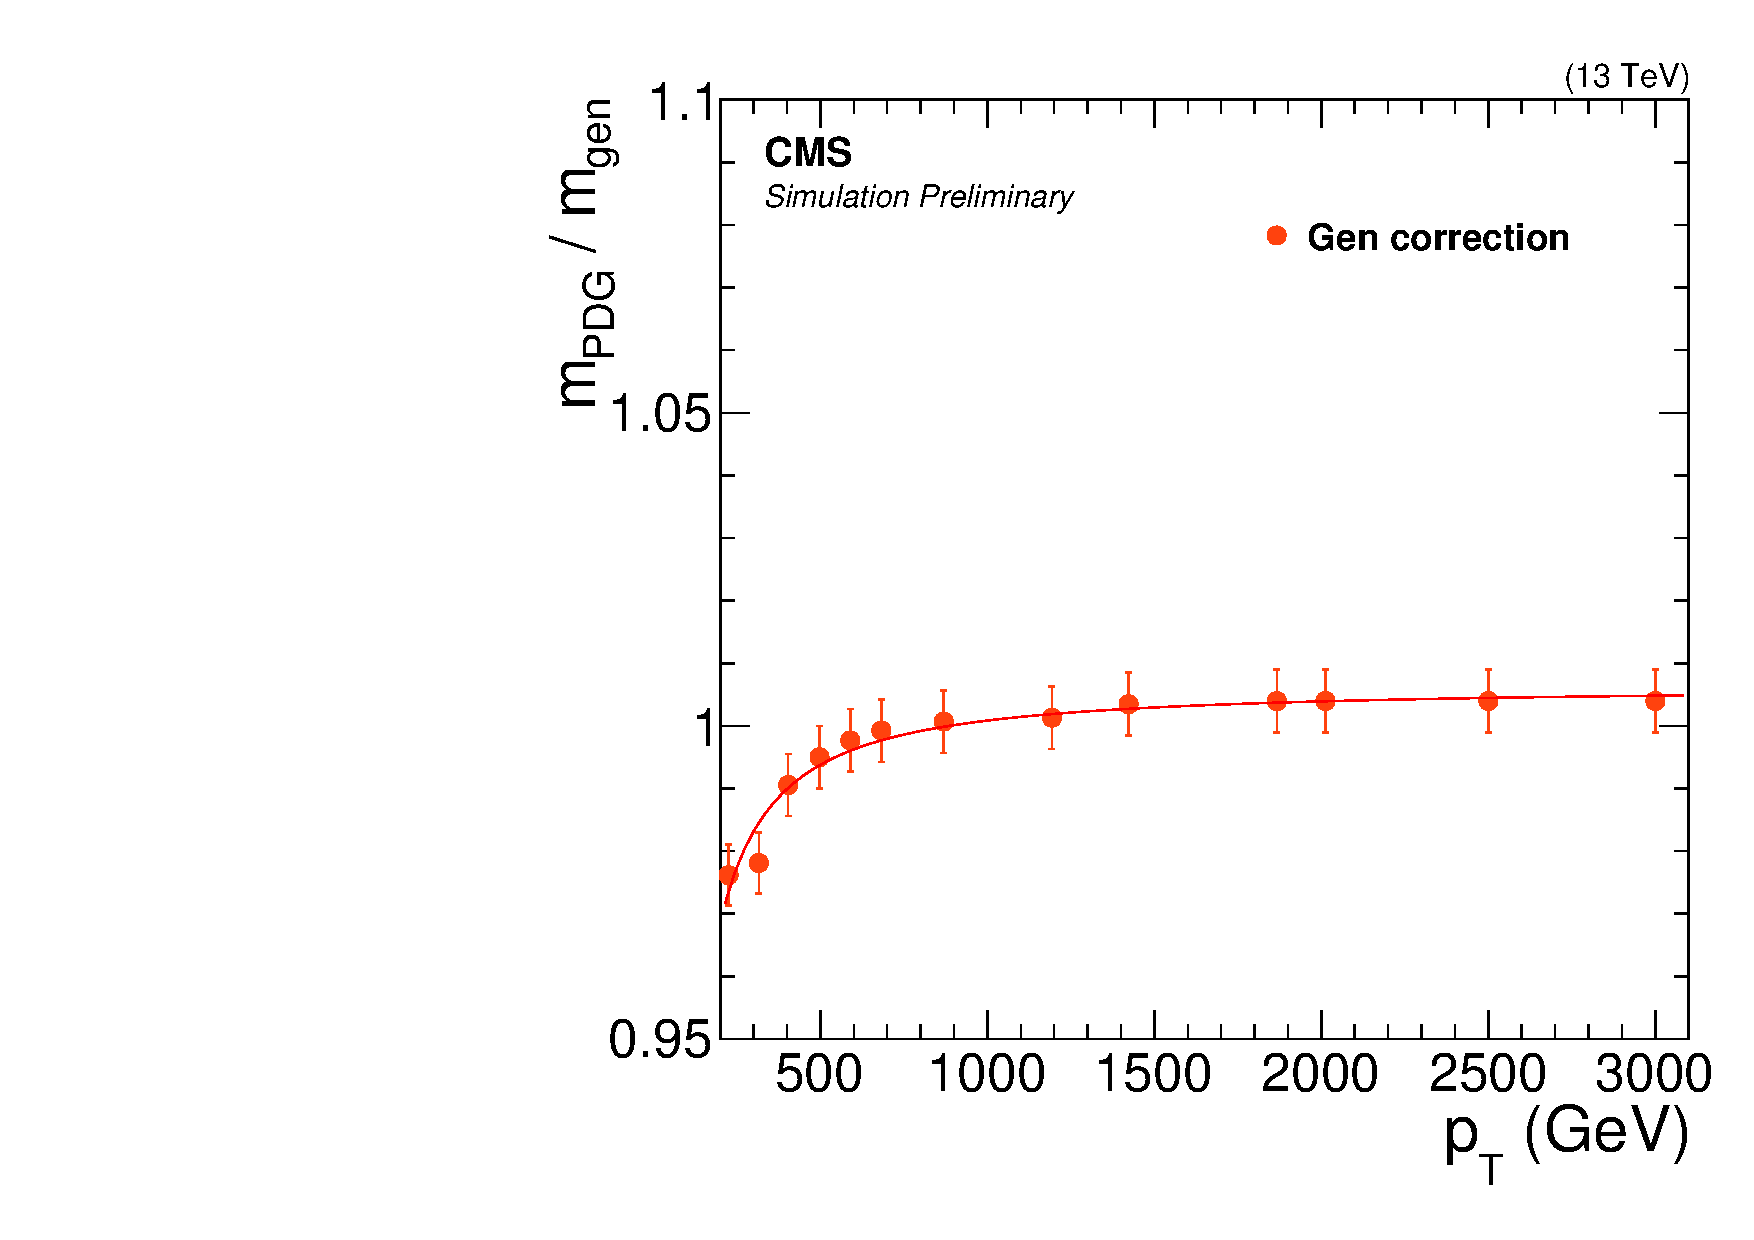
\includegraphics[width=0.45\textwidth]{figures/analysis/search2/AN-16-235/plots/JMC_fit_gen.pdf}
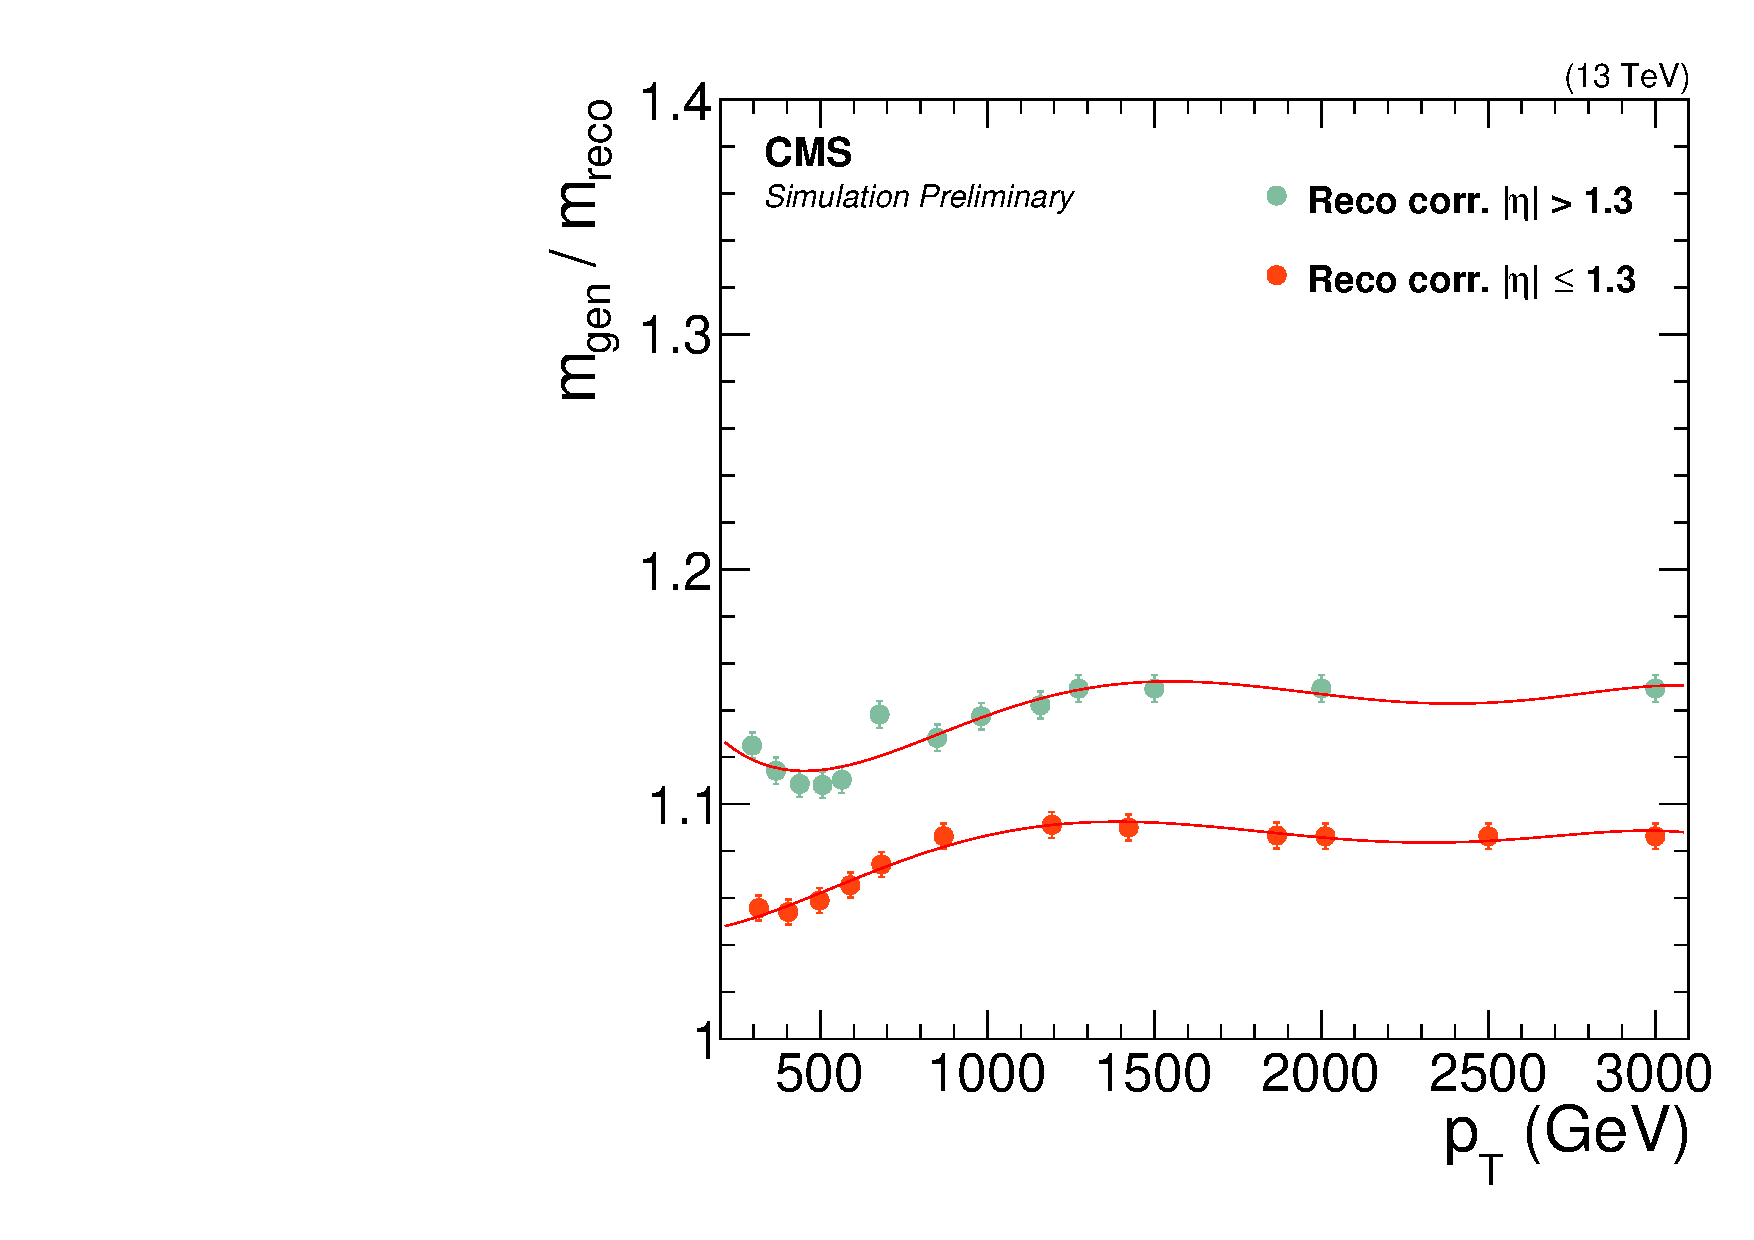
\includegraphics[width=0.45\textwidth]{figures/analysis/search2/AN-16-235/plots/JMC_fit_reco.pdf}
\caption{Fit to $\rm{M_{PDG}/M_{GEN}}$ as a function of jet $\pt$ (left), where $\rm{M_{PDG}}=80.4~\GeV$ and $\rm{M_{GEN}}$ is the fitted mean of the generator level mass and a fit to $\rm{(M_{RECO}-M_{GEN})/M_{RECO}}$ (right), where $\rm{M_{RECO}}$ is the reconstructed softdrop mass, as a function of jet $\pt$ in two $\eta$ bins.}
\label{fig:jmcfits}
\end{figure}

The two corrections are then applied to the uncorrected PUPPI softdrop mass both in data and in MC as
\begin{equation}
M_{SD}=M_{\rm{SD, uncorr}} \times \rm{w_{GEN}} \times \rm{w_{RECO}}
\end{equation}
where $w_{GEN}$ and $w_{RECO}$ correspond to the gen and reco corrections respectively and $M_{\rm{SD, uncorr}}$ is the uncorrected PUPPI softdrop mass. \par

  
Finally, a closure test is performed in order to check that the corrected PUPPI+softdrop W-jet mass peaks at 80.4 \GeV and is stable with \PT and $\eta$. The fitted mean of the corrected PUPPI softdrop mass peak as a function of jet \PT in two different $\eta$ bins is shown in Figure~\ref{fig:searchII:wtagclosure}. Good closure is observed, with the corrected mass peaking around 80 GeV independent of the jet $\pt$ and $\eta$.The PUPPI softdrop jet mass peak for W/Z-jets from different signal samples after jet mass corrections have been applied is shown in Figure~\ref{fig:search2:corrMass}, for resonances with a mass of 1 and 4 TeV. The corrections applied to Z-jets yield a mass stable with \PT, peaking around the Z mass. 
\begin{figure}[htbp]
\centering
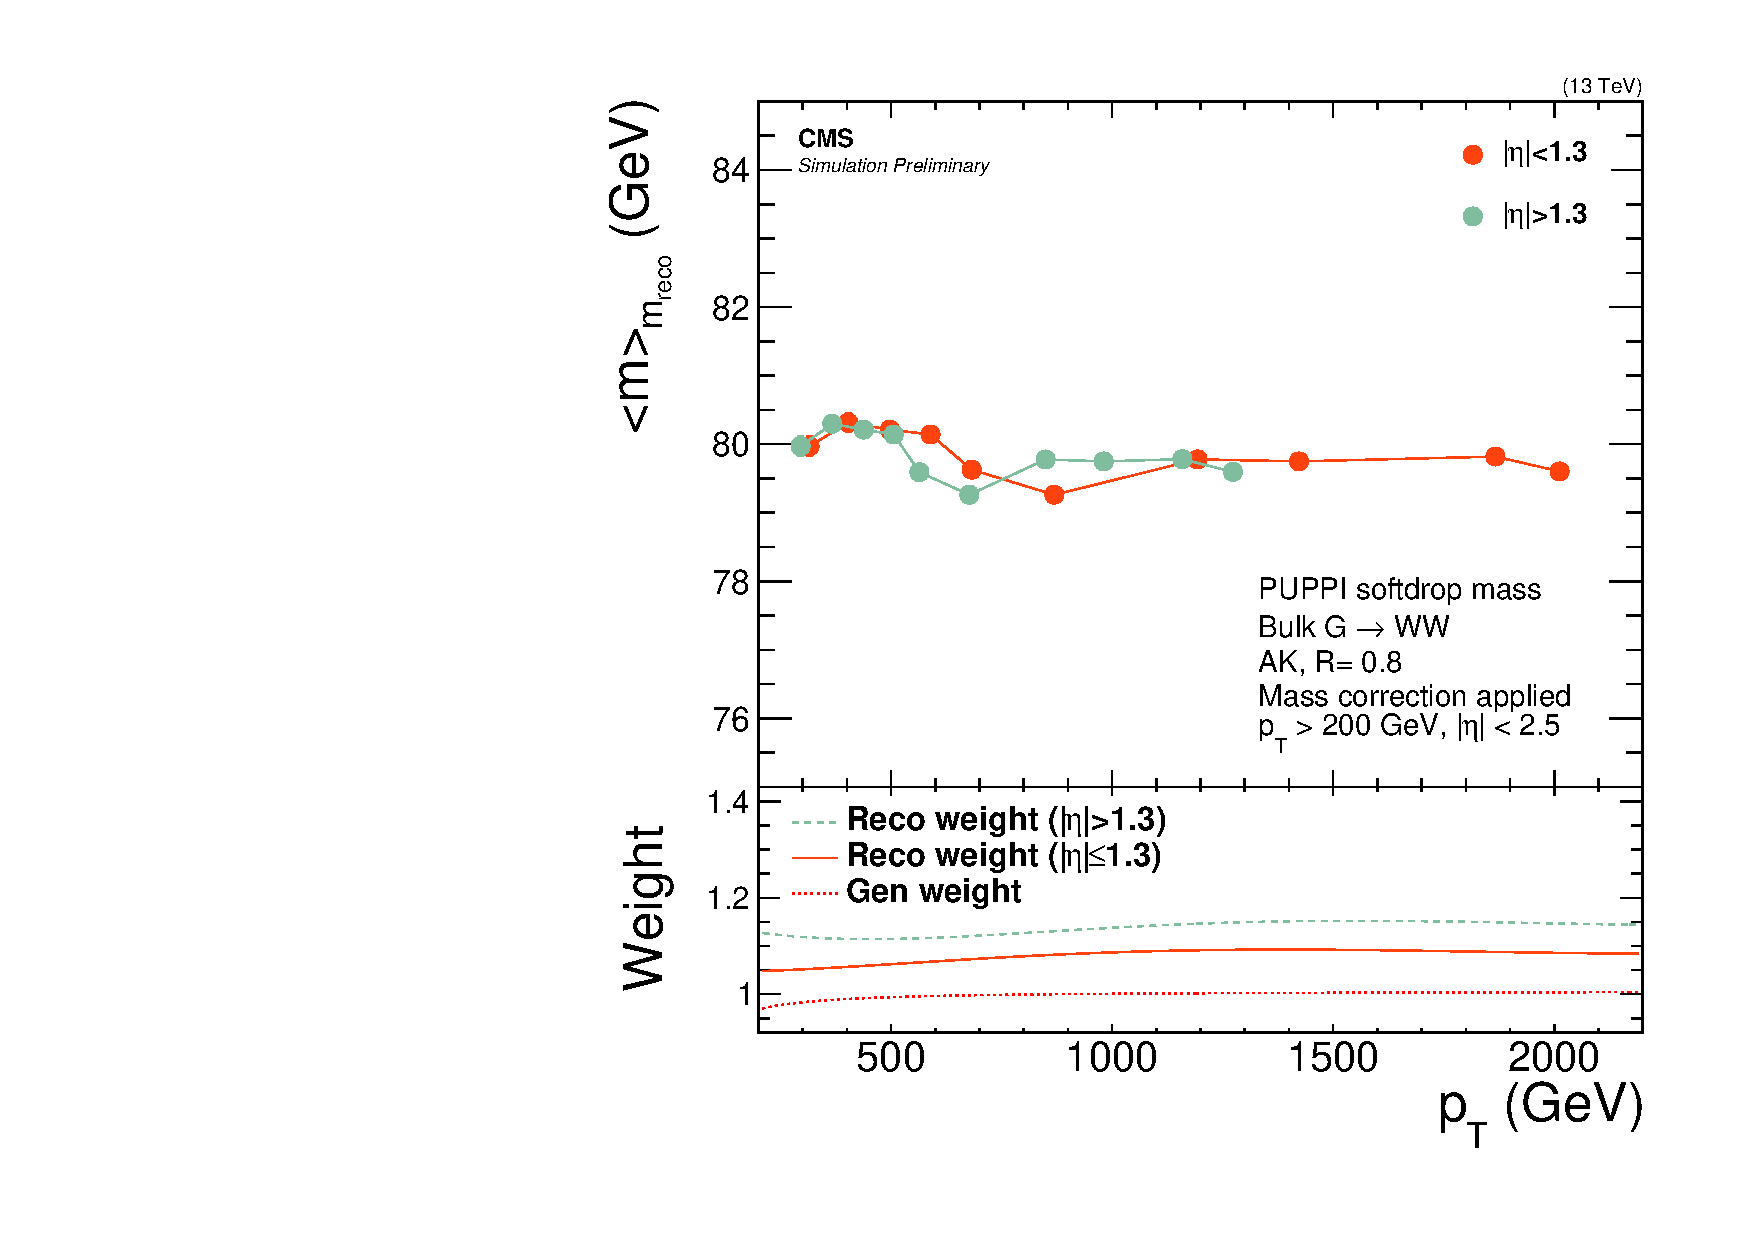
\includegraphics[width=0.49\textwidth]{figures/analysis/search2/AN-16-235/plots/ClosureTest_RecoMass.pdf}
\caption{The mean of the fitted W-jet corrected PUPPI softdrop mass peak as a function of jet $\pt$ in two different $\eta$ bins.}
\label{fig:searchII:wtagclosure}
\end{figure}

\begin{figure}[htbp]
\centering
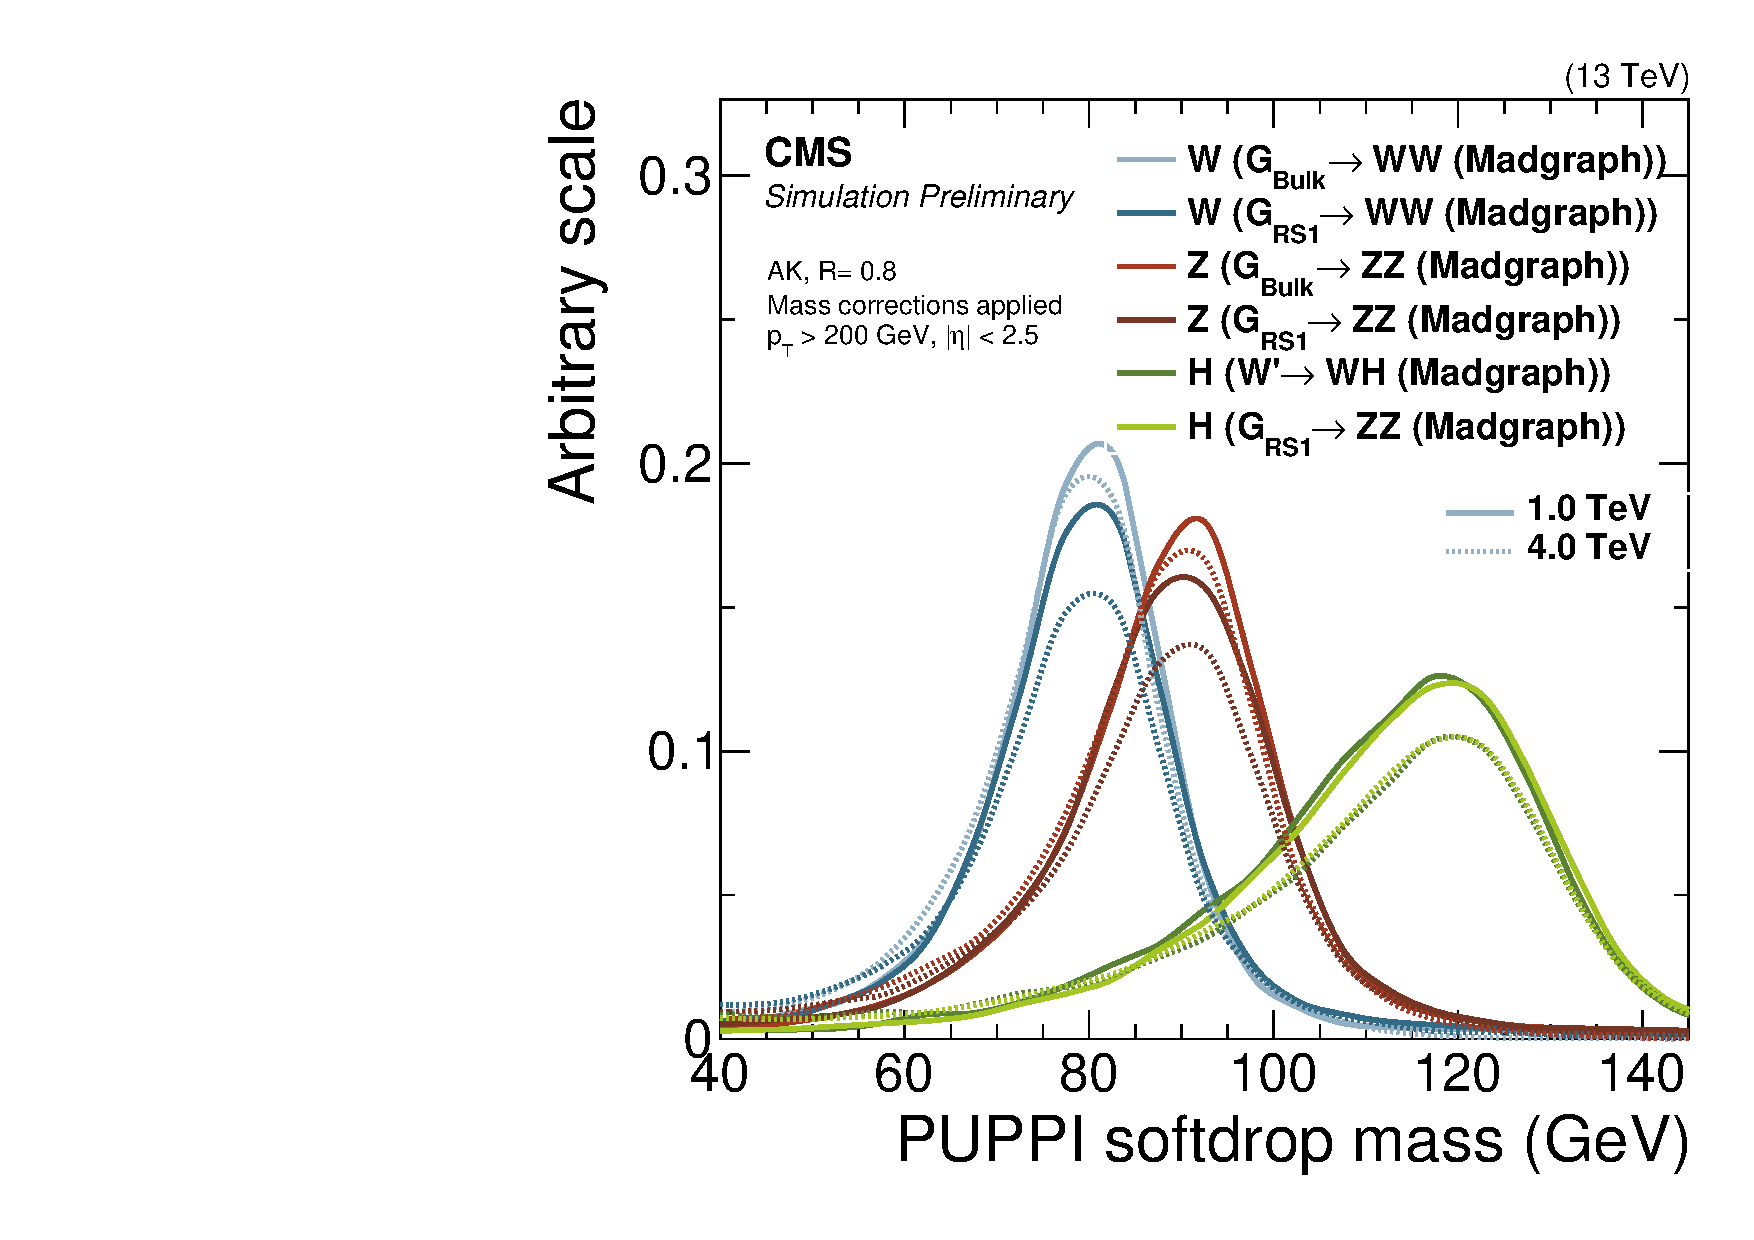
\includegraphics[width=0.49\textwidth]{figures/analysis/search2/AN-16-235/plots/SoftdropMass_NEWCORR_wH0.pdf}
\caption{The W/Z/H-jet corrected PUPPI softdrop mass peak for jets from different signal samples with masses of 1 and 4 TeV.}
\label{fig:search2:corrMass}
\end{figure}

\subsection{W-tagging performance}
The new PUPPI+softdrop based \PW/\PZ-tagger uses a mass window of $65 \GeV < m_{SD} < 105 \GeV$ in combination with a cut of PUPPI $\tau_{21}<0.4$.
We compare its performance to that of the CHS+pruning based tagger used in Search I as well as to that of a "DDT-transformed" \nsubj based tagger~\cite{Dolen:2016kst}. The $\tau_{21}^{DDT}$ variable is a linear transformation of \nsubj given as
\begin{equation}
\tau_{21}^{DDT} = \tau_{21} + M \times \log \bigg( \frac{m^2}{p_T \times 1 \textrm{ GeV}}\bigg)
\end{equation}
where $M=-0.063$ is obtained from a fit of $\tau_{21}$ against the variable $\rho^{'}=\log(m^2/\PT/\mu)$, where $\mu = 1 \GeV$.
The purpose of this is to decorrelate $\tau_{21}$ from the softdrop mass and \PT, yielding a mass and dijet invariant mass spectrum minimally sculpted by
a cut on the $\tau_{21}^{DDT}$ tagging variable. This is tagger that will be further explored and explained in detail in the context of Search III, Section~\ref{sec:searchIII:ddt}.\par
The background rejection efficiency for QCD light flavor jets as a function of W-jet signal efficiency is shown in Figure~\ref{fig:searchII:roc}
The efficiency is measured requiring a fixed jet mass window of 65-105 \GeV, while scanning the cut on $\tau_2/\tau_1$.

\begin{figure}[htbp]
\centering
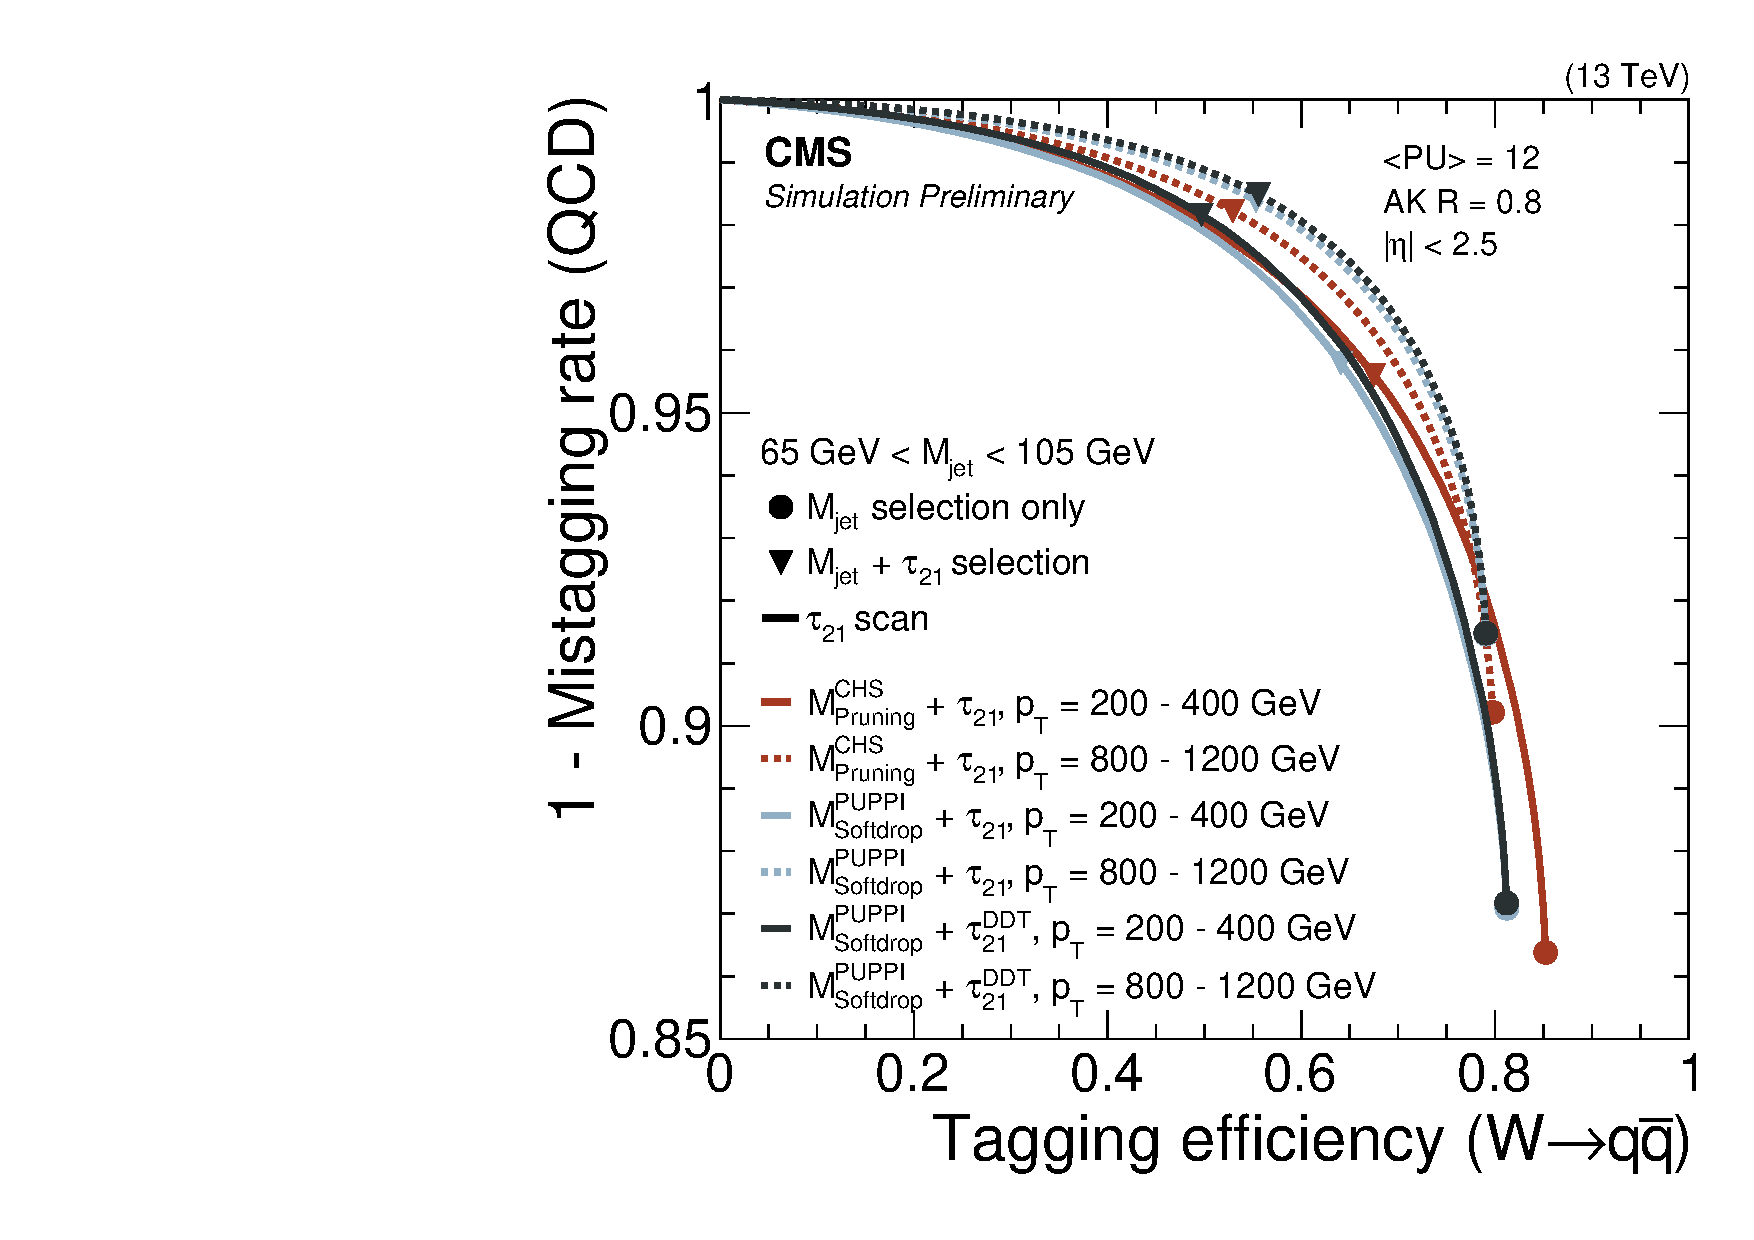
\includegraphics[width=0.49\textwidth]{figures/vtagging/JME-16-003/BoostedW/roc_WqqvsQCD_2bins.pdf}
\caption{The background rejection efficiency for QCD light flavor jets as a function of W-jet signal efficiency. A cut on CHS pruned or PUPPI softdrop jet
mass of $65<m_{\mathrm{jet}}<105$~\GeV is applied while scanning the cut on \nsubj. The cuts corresponding to $\tau_2/\tau_1 < 0.45$ for CHS+pruning, PUPPI $\tau_2/\tau_1 < 0.4$ for PUPPI+softdrop or $\tau_{21}^\text{DDT}<0.52$ are indicated with triangles, while the solid circles represent the efficiency and mistag rate for a mass cut only.
}
\label{fig:searchII:roc}
\end{figure}

The general performance of each tagger is very similar, with the PUPPI+softdrop based taggers displaying a slightly higher signal efficiency for a given mistag rate at high \PT and CHS+pruning slightly better at low \PT.
Two better understand the difference between each tagger, we look at the tagging performance as a function of jet \PT as well as pileup, shown in Figure~\ref{fig:searchII:effvspt} and~\ref{fig:searchII:effvspu}.\par
Starting with the tagger \PT-dependence in Figure~\ref{fig:searchII:effvspt}, we observe that she signal efficiency of a PUPPI+softdrop of CHS+pruned jet mass cut is flat as a function of \PT, at around 80\%. The QCD mistagging rate drops for both groomers, with a 1-3\% lower mistag rate using PUPPI+softdrop that CHS+pruning.

\begin{figure}[h!]
\centering
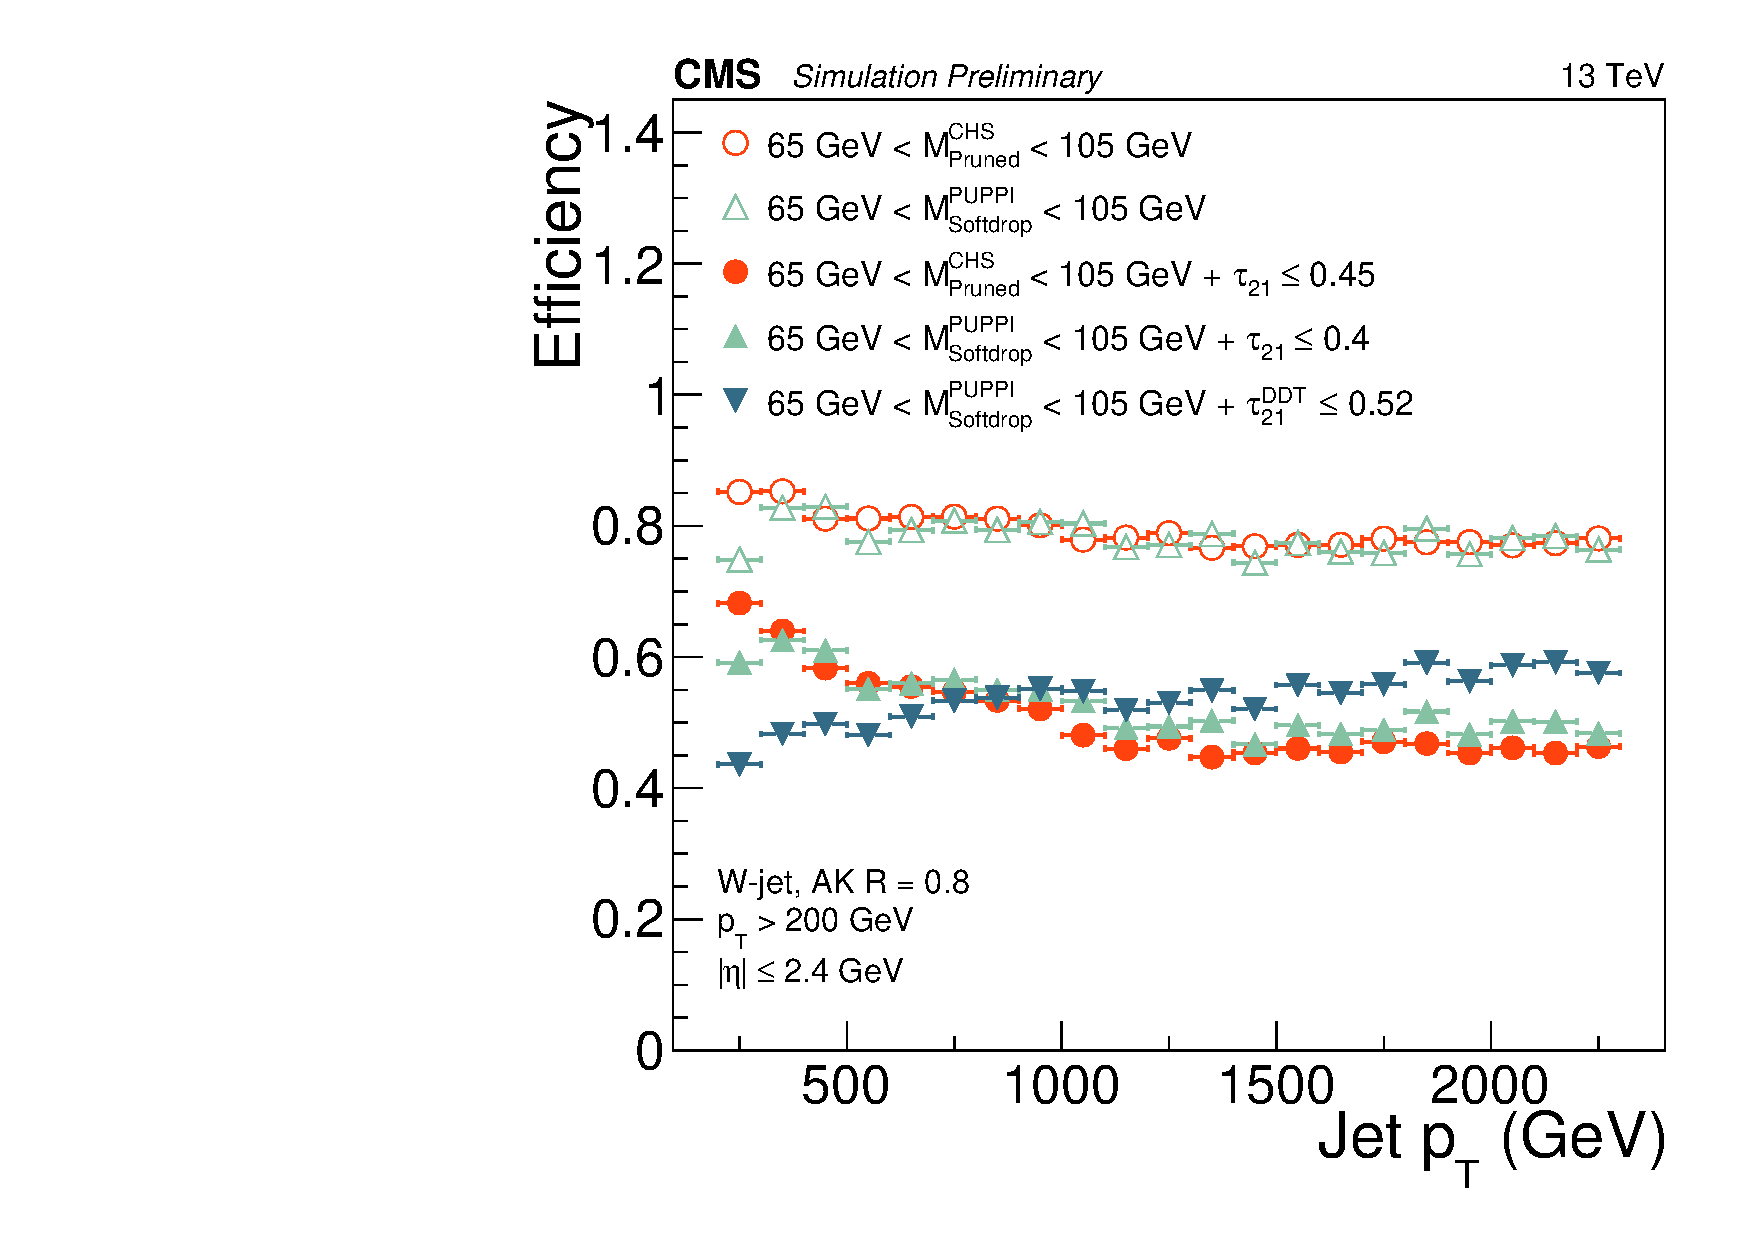
\includegraphics[width=0.49\textwidth]{figures/vtagging/JME-16-003/BoostedW/WtagSigEffvsPT.pdf}
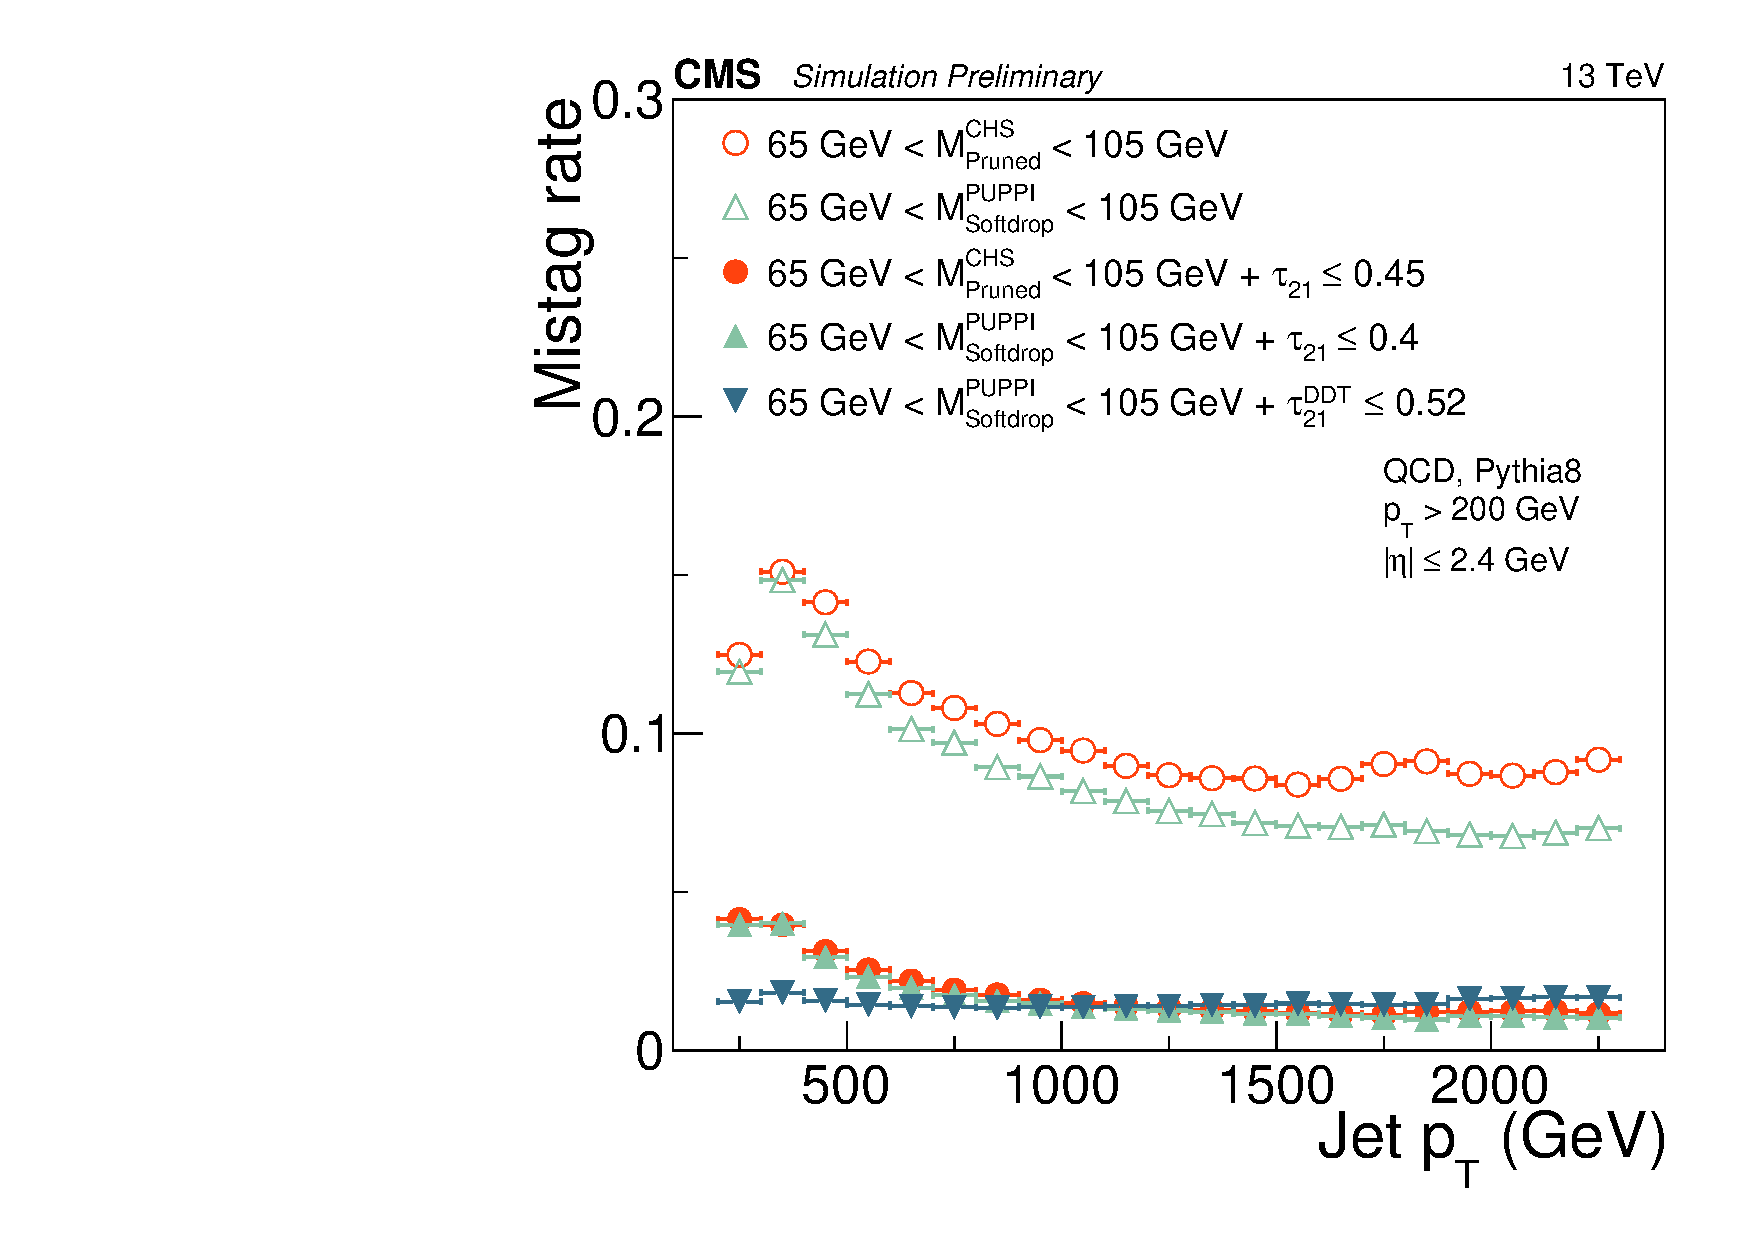
\includegraphics[width=0.49\textwidth]{figures/vtagging/JME-16-003/BoostedW/QCDBkgEffvsPT.pdf}
\caption{W-jet efficiency (left) and QCD light jet mistag rate (right) for a PUPPI+softdrop or CHS+pruned jet mass selection only (hollow circles) and the combined $m_{\mathrm{jet}}$ + (PUPPI) $\tau_2/\tau_1$ (DDT) selection (solid circles) as a function of jet \PT.}
\label{fig:searchII:effvspt}
\end{figure}

Once applying a \nsubj cut, the signal efficiency as well as the mistag rate for the PUPPI \nsubj and CHS \nsubj taggers drops as a function of \PT, with an average signal efficiency of around 50\% for a $\sim 2\%$ mistag rate. An interesting behavior is observed for the $\tau_{21}^{DDT}$ tagger: While the mistag rate is flat as a function of \PT, as is the purpose of decorrelated taggers, the signal efficiency improves as the \PT increases, outperforming the other taggers above 1 \TeV. \par
Turning to the tagger pileup dependence, shown in Figure~\ref{fig:searchII:effvspu}, the expected benefit from using the PUPPI algorithm is observed: The tagging efficiency for the CHS+pruning (red solid cirles) based tagger falls of steeply versus the number of primary vertices in the event, while the PUPPI+softdrop based taggers (light and dark blue solid circles) are insensitive to pileup.


\begin{figure}[htbp]
\centering
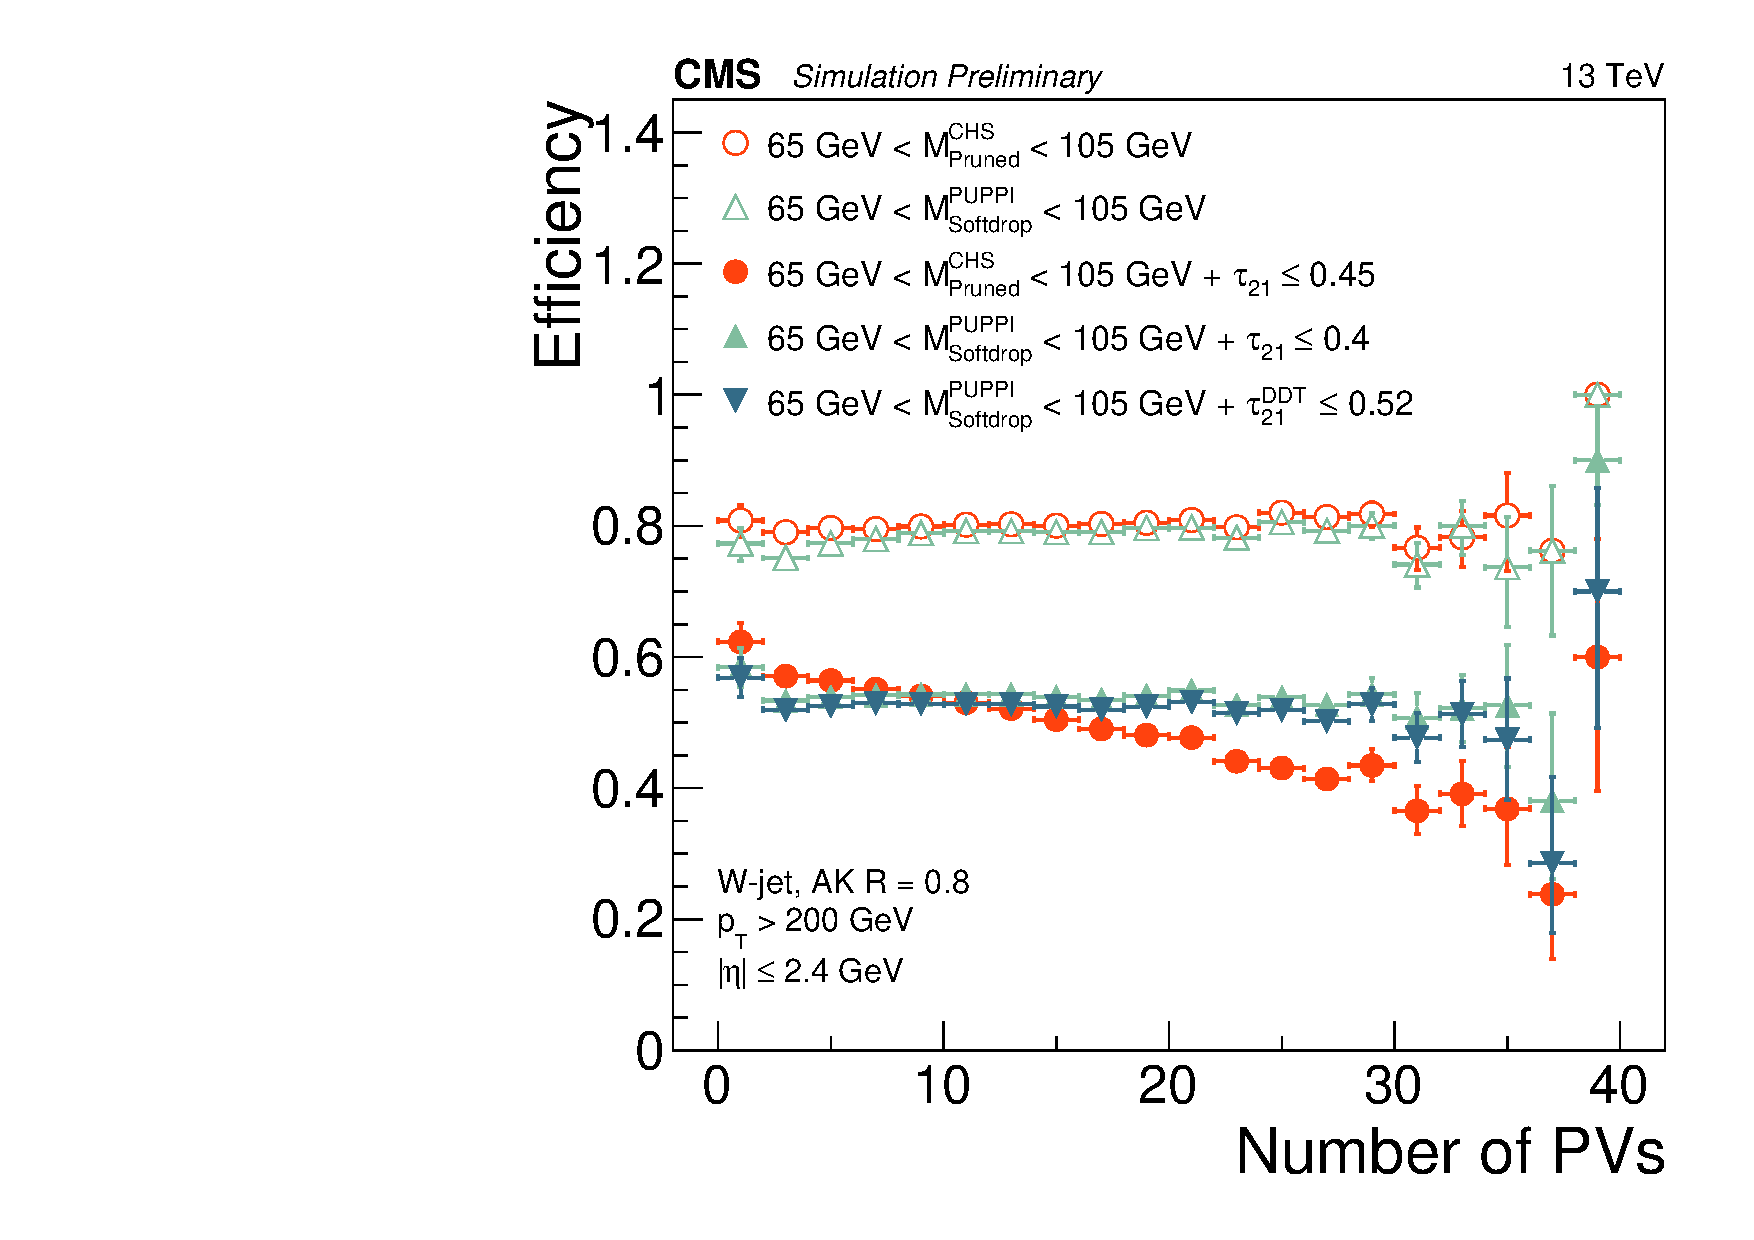
\includegraphics[width=0.49\textwidth]{figures/vtagging/JME-16-003/BoostedW/WtagSigEffvsNPV.pdf}
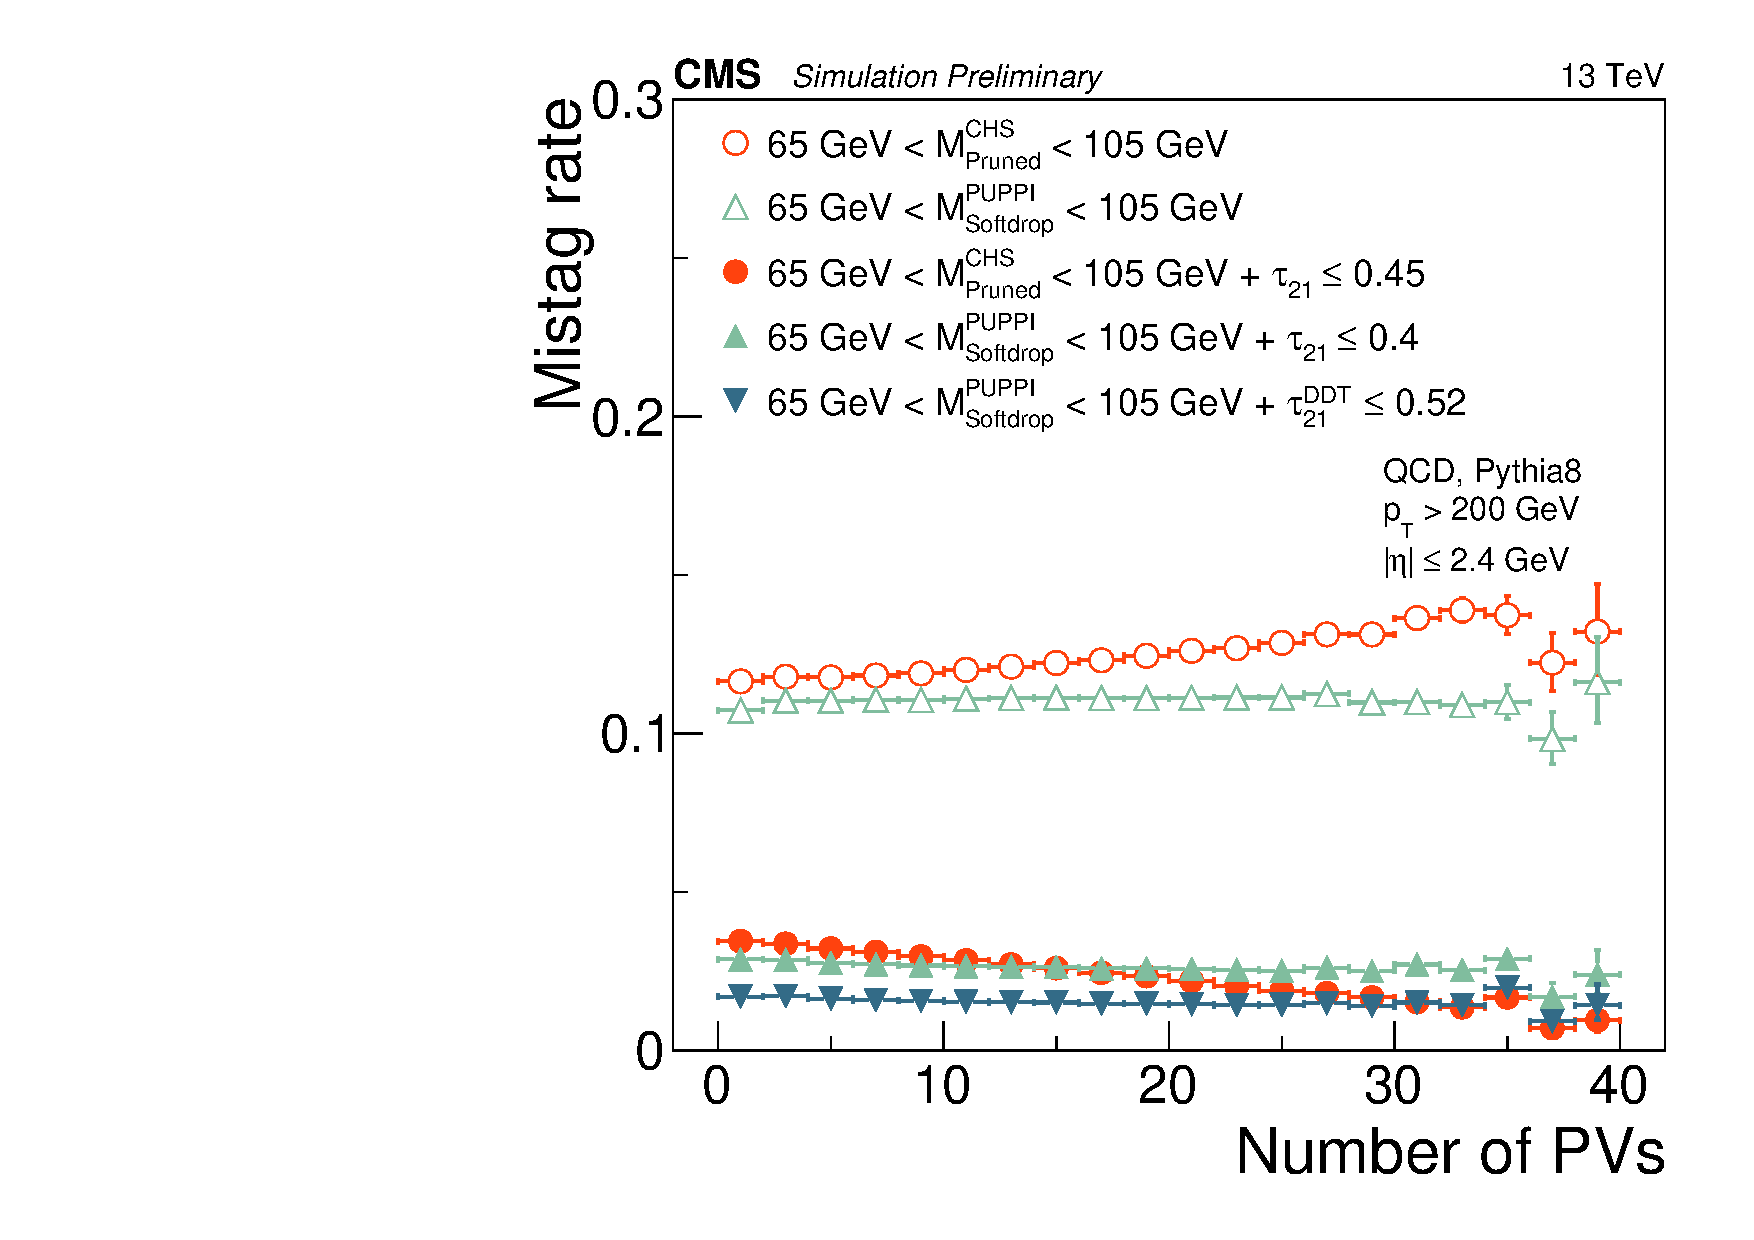
\includegraphics[width=0.49\textwidth]{figures/vtagging/JME-16-003/BoostedW/QCDBkgEffvsNPV.pdf}
\caption{W-jet efficiency (left) and QCD light jet mistag rate (right) for a PUPPI+softdrop or CHS+pruned jet mass selection only (hollow circles) and the combined $m_{\mathrm{jet}}$ + (PUPPI) $\tau_2/\tau_1$ (DDT) selection (solid circles) as a function of jet pileup.}
\label{fig:searchII:effvspu}
\end{figure}

   
\subsection{Validation in data}  
  

